\documentclass[a4paper, twoside, 12pt]{book}
%\usepackage[margin=3cm]{geometry}
%\usepackage[pdftex]{graphicx}
\usepackage{graphicx}
\graphicspath{{obr/}{obr/plots/}{spice/}}
\DeclareGraphicsExtensions{.ps, .eps}
\usepackage[slovak]{babel}
\usepackage[utf8]{inputenc} 
%\usepackage[T1]{fontenc}

\usepackage{amsmath}

\usepackage{listings}
\lstset{basicstyle=\ttfamily\footnotesize, breaklines=true}

%\usepackage[hidelinks]{hyperref}
\usepackage[breaklinks]{hyperref}

\usepackage{color} % kvoli epslatex obrazkom z octave

\usepackage{lettrine}

\usepackage{microtype}
%\usepackage[activate={true,nocompatibility},final,tracking=true,kerning=true,spacing=true,factor=1100,stretch=10,shrink=10]{microtype}
% activate={true,nocompatibility} - activate protrusion and expansion
% final - enable microtype; use ``draft'' to disable
% tracking=true, kerning=true, spacing=true - activate these techniques
% factor=1100 - add 10% to the protrusion amount (default is 1000)
% stretch=10, shrink=10 - reduce stretchability/shrinkability (default is 20/20)

%\usepackage[section]{placeins}
\usepackage{placeins}

%\usepackage{boisik}
%\usepackage{baskervald}
\usepackage{fourier}
%\usepackage{baskervald}
%\usepackage[charter]{mathdesign}
\usepackage{Baskervaldx}	% funguje aj smallcaps: \textsc 
%\usepackage[lining]{ebgaramond}	% lining - cisla nie oldstyle
%\usepackage{concmath}
%\usepackage[charter]{mathdesign}

%\usepackage[lf]{Baskervaldx} % lining figures
%\usepackage[bigdelims,vvarbb]{newtxmath} % math italic letters from Nimbus Roman
%\usepackage[cal=boondoxo]{mathalfa} % mathcal from STIX, unslanted a bit
%\renewcommand*\oldstylenums[1]{\textosf{#1}}

%\usepackage[urw-garamond]{mathdesign}
%\usepackage[T1]{fontenc}

\pagestyle{headings}

%% velkost fontu pod obrazkom mensia, vratane ``Obr. X:''
%\renewcommand{\figurename}{sjls} % toto nefunguje pri pouzivani babel
\addto\captionsslovak{\renewcommand{\figurename}{\small Obr.}}
%\renewcommand{\thefigure}{\small \arabic{figure}}
%\renewcommand{\thefigure}{\small \arabic{chapter}.\arabic{figure}}
\renewcommand{\thefigure}{\small \thechapter.\arabic{figure}}


\newcommand{\dif}{\, \mathrm{d}}	% diferencia (na derivacie)
\newcommand{\difp}{\partial}		% parc. diferencia 
\newcommand{\dxdt}[2]{\frac{\mathrm{d} #1}{\mathrm{d} #2}}
\newcommand{\dxdtp}[2]{\frac{\partial #1}{\partial #2}}
\newcommand{\un}[1]{\, \mathrm{#1}}	% jednotky velicin, v math mode
\newcommand{\E}[1]{\cdot 10^{#1}}
\newcommand{\degree}{^\circ}
\newcommand{\diameter}{\emptyset}
\newcommand{\cpx}{\widehat}		% komplexne fazory
\newcommand{\Ohm}{\Omega}


\newcounter{myasscount}
\renewcommand{\themyasscount}{\alph{myasscount}}
%\setcounter{myasscount}{1}
\newenvironment{myass}
{

	\refstepcounter{myasscount}
	\par
	\vspace{6pt}
	%\indent	% netreba, ked predchadza \par
	\begin{tabular}{p{.22\textwidth}  p{.68\textwidth} }
	\textbf{Predpoklad (\themyasscount)}	&
}
{
	\end{tabular}
	\par 
	\vspace{6pt}
}

\newcommand{\myfig}[3]
{
    \begin{figure}[!ht]
	\centering
	\includegraphics{#1}
	\caption{#2}
	%\label{fig:#3}
	#3
    \end{figure}
}

\newcommand{\myfigtex}[3]
{
    \begin{figure}[!ht]
	\centering
	\input{#1}
	\caption{#2}
	%\label{fig:#3}
	#3
    \end{figure}
}

\newcommand{\myfigschplot}[4]
{
    \begin{figure}[!ht]
	\centering
	\includegraphics{#1} 	% obrazok - simulacna schema
	\input{#2} 	% obrazok - priebehy
	\caption{#3}
	%\label{fig:#4}
	#4
    \end{figure}
}

\newcommand{\myfigschplottex}[4]
{
    \begin{figure}[!ht]
	\centering
	\input{#1} 	% obrazok - schema
	\input{#2} 	% obrazok - priebehy
	\caption{#3}
	%\label{fig:#4}
	#4 		% label
    \end{figure}
}

\newcommand{\myfigschplotplottex}[5]
{
    \begin{figure}[!ht]
	\centering
	\input{#1}\\	% obrazok - schema
	\input{#2}\\ 	% obrazok - priebehy1
	\hspace{0mm}\input{#3} 	% obrazok - priebehy2
	\caption{#4}
	%\label{fig:#5}
	#5 		% label
    \end{figure}
}

\newcommand{\xcll}[2]{\def#1{\ifmmode \text{#2} \else #2 \fi}}

\xcll{\llgt}{$t$}
\xcll{\llgUd}{$U_d$}
\xcll{\llgton}{$t_{on}$}
\xcll{\llgtoff}{$t_{off}$}

\xcll{\llgTonj}{$T_{on,1}$}
\xcll{\llgToffj}{$T_{off,1}$}
\xcll{\llgTond}{$T_{on,2}$}
\xcll{\llgtj}{$t_1$}
\xcll{\llgtd}{$t_2$}

\xcll{\llgvg}{$u_G$}
\xcll{\llgvce}{$u_{CE}$}
\xcll{\llgvL}{$u_L$}
\xcll{\llgic}{$i_C$}
\xcll{\llgiD}{$i_D$}
\xcll{\llgiL}{$i_L$}
\xcll{\llgiK}{$i_K$}
\xcll{\llgIc}{$I_C$}

\xcll{\llUmerBmax}{$\approx B_{max}$}

%% prudove_trafo_model
\xcll{\llgud}{$u_2$}
\xcll{\llgij}{$i_1$}
\xcll{\llgudb}{$u_2^,$}
\xcll{\llgidk}{$i_{2,K}$}
\xcll{\llgimag}{$i_\mu$}

\xcll{\llgRcu}{$R_{Cu}$}
\xcll{\llgRb}{$R_b$}

% % % % % % % % % % 
%%% model %%%
\xcll{\llgxi}{$x_i$}
\xcll{\llgxio}{$x_{i+1}$}
\xcll{\llgyj}{$y_j$}
\xcll{\llgyjo}{$y_{j+1}$}
\xcll{\llgfij}{$f_{i,j}$}
\xcll{\llgfioj}{$f_{i+1,j}$}
\xcll{\llgfijo}{$f_{i,j+1}$}
\xcll{\llgfiojo}{$f_{i+1,j+1}$}




\xcll{\llaR}{R$\cdot \dif x$}
\xcll{\llaL}{L$\cdot \dif x$}
\xcll{\llaG}{G$\cdot \dif x$}
\xcll{\llaC}{C$\cdot \dif x$}
\xcll{\llai}{$i$}
\xcll{\llau}{$u$}
\xcll{\llaidi}{$i + \dxdtp{i}{x} \dif x$}
\xcll{\llaudu}{$u + \dxdtp{u}{x} \dif x$}
\xcll{\llaGen}{generátor}
\xcll{\llaZat}{spotrebič}
\xcll{\lladx}{$\dif x$}



\begin{document}


%\maketitle

\newcommand{\nazov}{\textit{Výkonové spínací tranzistory} }
\newcommand{\typprace}{diplomov}


%%%%%%%%%%%%%%%%%%%%%%%%%%
%%	TITULNY LIST	%%
%%%%%%%%%%%%%%%%%%%%%%%%%%
\thispagestyle{empty}

%\begin{minipage}[t]{.16\textwidth}
%	\includegraphics[width=.8\textwidth]{kapitoly/logoVUT} \ \
%\end{minipage}
%\begin{minipage}[t][t]{.5\textwidth}
%	alkalkja
%
%	a,a,a,a,
%	llkfdj
%
%	sdlojsdlj
%
%	slkdldsjk
%\end{minipage}

%\noindent
%\begin{tabular}{p{.16\textwidth}  p{.8\textwidth} }
%	\vspace{48pt}\includegraphics[width=.16\textwidth]{kapitoly/logoVUT} & 
%	\large\textsc{Vysoké učení technické v~Brně} \newline \footnotesize{} \newline
%	\normalsize\textsc{Brno University of Technology}
%\end{tabular}
%\par

%%\vspace{6pt}
%\noindent
%\begin{tabular}{p{.16\textwidth}  p{.8\textwidth} }
%	\vspace{56pt}\includegraphics[width=.16\textwidth]{kapitoly/logoFEKT} & 
%	\normalsize\textsc{Fakulta elektrotechniky a komunikačních technologií} \newline
%	\normalsize\textsc{Ústav výkonové elektrotechniky a elektroniky} \newline
%	\newline 
%	\small\textsc{Faculty of Electrical Engineering and Communication} \newline
%	\small\textsc{Department of Power Electrical and Electronic Engineering}
%\end{tabular}
%\par

%\vspace{96pt}
%%\centering
%\begin{center}
%\LARGE\textsc{\textbf{Výkonové spínací tranzistory\\}}
%\vspace{12pt}
%\large\textsc{Power Switching Transistors}
%\end{center}
%\par
%
%\vspace{120pt}
%\noindent
%\begin{tabular}{p{.40\textwidth}  p{.60\textwidth} }
%	\large\textsc{Semestrální práce}\newline
%	\normalsize\textsc{Semestral Thesis}\\
%	\\
%	\large\textsc{Autor práce}\newline
%	\normalsize\textsc{Author}		&	\normalsize Bc. \textsc{Ján Mikláš}\\
%	\\
%	\large\textsc{Vedoucí práce}\newline
%	\normalsize\textsc{Supervisor}		&	\normalsize doc. Dr. Ing. \textsc{Miroslav Patočka}\\
%	\\
%	\\
%	\normalsize\textsc{Brno 2016}
%\end{tabular}
%\par
%\normalsize


\includegraphics[height=\textheight]{TitulniList_black-crop}

\newpage\thispagestyle{empty}\mbox{}
% cista strana - kvoli obojstrannej tlaci a zadaniu


\newpage
%%%%%%%%%%%%%%%%%%%%%%%%%%%%%%%%%%%%%%%%%%%%%%%%%%%%%%%%ť

%\thispagestyle{empty}
%includegraphics[height=\textheight]{kapitoly/titulnylist-crop}
%\newpage
\thispagestyle{empty}
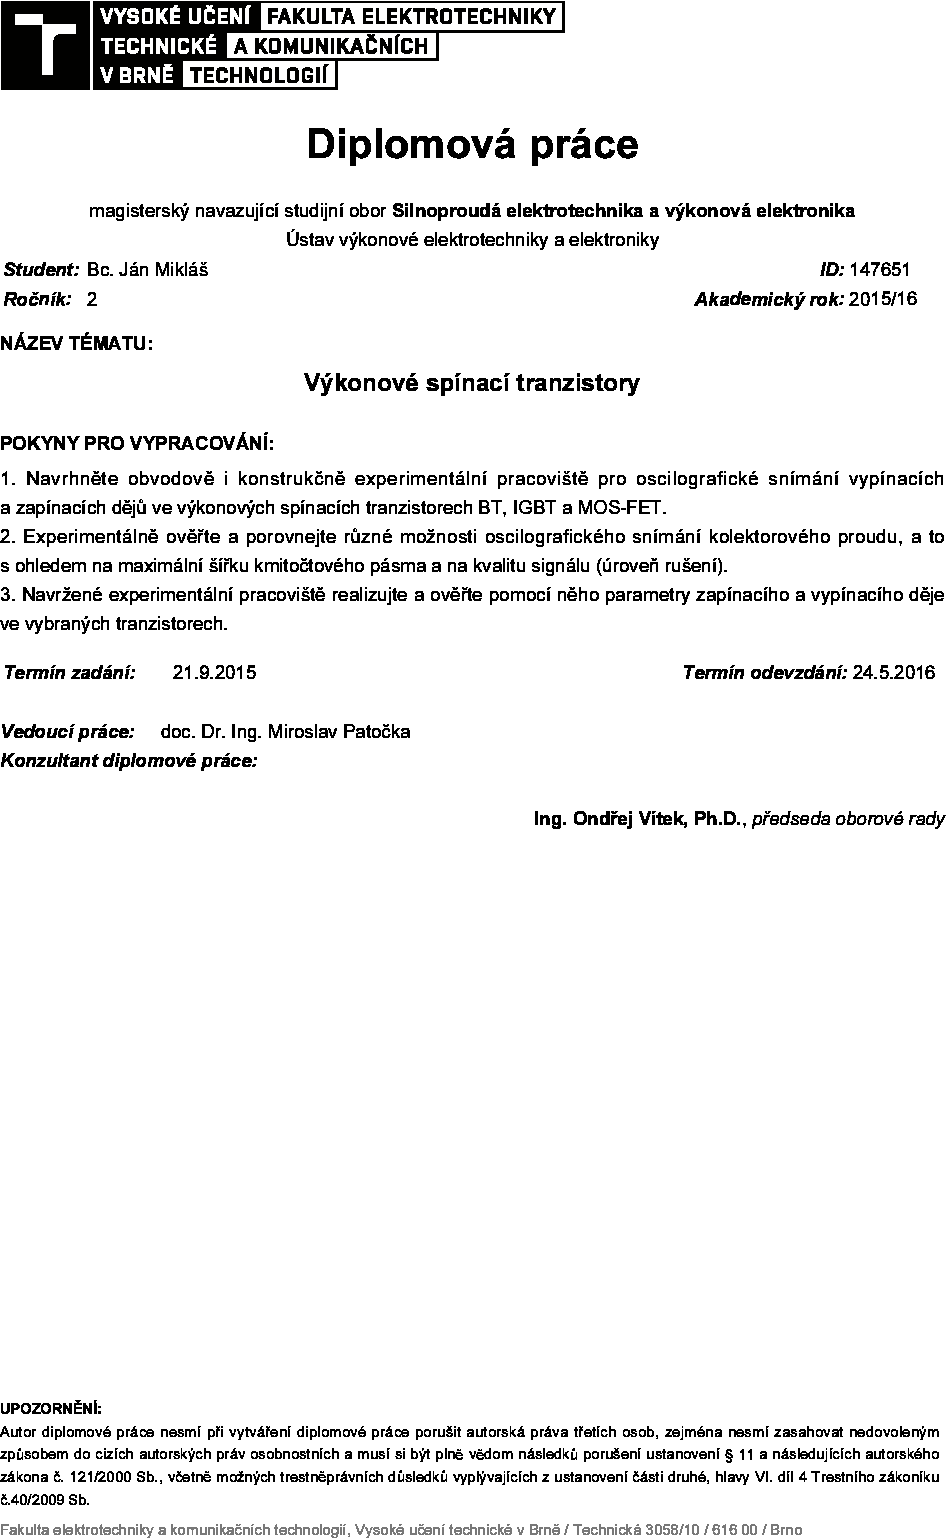
\includegraphics[width=\textwidth]{zadanieDP-crop}




\newpage\thispagestyle{empty}\mbox{}
% cista strana - kvoli obojstrannej tlaci a zadaniu

\newpage\thispagestyle{empty}\mbox{}


\newpage
\thispagestyle{empty}
\section*{Kľúčové slová}
výkonové spínacie tranzistory, spínacie straty, priebehy zapínacieho deja, priebehy vypínacieho deja, meranie spínacích strát, snímanie prúdu, simulačný model spínacieho tranzistora
\vspace{30mm}
\section*{Keywords}
power switching transistor, switching loss, turn on waveform, turn off waveform, switching loss measurements, current sensor, switching transistor simulation model

\newpage
\thispagestyle{empty}
\section*{Abstrakt}
V práci sú popísané predpoklady meraní spínacích strát, ktoré boli vykonané v rámci práce a je navrhnutý napäťový medziobvod a budič výkonových tranzistorov.

Nasleduje odvodenie funkcie aproximujúcej priebeh vodivosti $g_{CE} = \frac{i_C}{u_{CE}}$, ukážky simulácie spínacích dejov pomocou tejto vodivosti a pojednanie o zmeraných priebehoch.

\paragraph{}


\section*{Abstract}
In this thesis, prerequisities for a switching loss measurements  are established as well as designing of DC-bus and the base/gate driver for the power transistors; followed by derivation of  mathematical approximation of transistor conductivity $g_{CE} = \frac{i_C}{u_{CE}}$, circuit simulation using $g_{CE}$ as a transistor model and a discussion of measured waveforms.



\newpage
\thispagestyle{empty}
\section*{Bibliografická citácia}
MIKLÁŠ, J. \nazov. Brno: Vysoké učení technické v~Brně, Fakulta elektrotechniky a komunikačních technologií, 2016. \pageref{LastPage} s. Vedoucí diplomové práce doc. Dr. Ing. Miroslav Patočka.

\newpage
\thispagestyle{empty}
\section*{Prehlásenie}

Prehlasujem, že svoju diplomovú~prácu na tému \nazov som vypracoval samostatne pod vedením vedúceho \typprace ej práce a s~použitím odbornej literatúry a ďalších informačných zdrojov, ktoré sú všetky citované a uvedené v~zozname literatúry na konci práce.
Ako autor uvedenej \typprace ej práce ďalej prehlasujem, že v~súvislosti s~vytvorením tejto práce som neporušil autorské práva tretích osôb, predovšetkým som nezasiahol nedovoleným spôsobom do cudzích autorských práv osobnostných a som si plne vedomý následkov porušenia ustanovenia § 11 a nasledujúcich autorského zákona č. 121/2000 Sb., včítane  možných
trestnoprávnych dôsledkov vyplývajúcich z~ustanovenia § 152 trestného zákona č. 140/1961 Sb.

\vspace{2cm}
V~Brne dňa \ldots\ldots\ldots\ldots\ldots \hspace{30mm}Podpis \ldots\ldots\ldots\ldots\ldots
%\vspace{5cm}



\newpage\thispagestyle{empty}\mbox{}

\section*{Poďakovanie}
Ďakujem v prvom rade vedúcemu práce doc. Dr. Ing. Miroslavovi Patočkovi za vecné, presné a účinné rady a vedenie v práci. Tiež ďakujem Ing. Petrovi Procházkovi, Ph.D. za ochotu a spoluprácu.


\tableofcontents
%\setcounter{page}{7}

\listoffigures


\chapter*{Úvod} \label{ch:uvod} \addcontentsline{toc}{chapter}{Úvod}
\markboth{\MakeUppercase{Úvod}}{\MakeUppercase{Úvod}} % aby to aj v hlavicke strany pisalo uvod a nie nieco predchadzajuce, napr. zoznam obrazkov


\lettrine{S}{pínacie} straty tvoria podstatnú časť celkových strát v spínacích polovodičových prvkoch pracujúcich pri vysokých frekvenciách. Ich analýza je preto prirodzene potrebná z hľadiska aplikačného ako aj pri vývoji súčiastok.

Analytické dynamické modely tranzistorov používané v bežných obvodových simuláciách, či už na základe \uv{charge control} prístupu (BJT, \cite{gummel-poon}, \cite{pierret}) alebo iné nie je možné použiť pre výkonové spínacie tranzistory. Behom spínania totiž prechádza tranzistor viacerými odlišnými režimami, ktorých hranice navyše nie sú ostro určené (podrobnejšie popisované napr. v \cite{baliga}), nehovoriac o skutočnej priestorovej komplexnosti polovodičových štruktúr oproti základným analytickým predstavám.

Pre jednotlivé typy spínacích tranzistorov existujú pomerne dôveryhodné ekvivalentné modely, ako napr. známy Hefnerov model \cite{hefner} IGBT tranzistora, ich použitie resp. zostavenie je však nie celkom priamočiare, čo môže byť zvlášť pre aplikačných inžinierov, ktorých zameraním nie sú obvodové simulácie či charakterizácia súčiastok, faktorom rozhodujúcim o samotnom použití alebo nepoužití simulátora.

Vedúci tejto práce so spolupracovníkmi \cite{valsa-patocka-petru} navrhli v časoch bipolárnych tranzistorov jednoduchú analýzu zmeraných spínacích priebehov pomocou predstavy časovo premennej vodivosti tranzistora $g_{CE}$. Táto predstava je natoľko základná, že nie je obmedzená na jeden konkrétny typ súčiastky, ale dá sa použiť (snáď s istými upresneniami) pre ľubovoľnú spínaciu súčiastku, teda aj moderné rýchle unipolárne tranzistory.

Konkrétnym spracovaním zmeraných priebehov a priebehu vodivosti $g_{CE}$ sa venuje podstatná časť tejto práce.

Samotné hodnoverné meranie prepínacích strát sa ostáva pri trende čoraz extrémnejších parametrov (rýchlosť, veľkosť prúdu) stále technickou výzvou.
Cieľom diplomovej práce je zostavenie meracieho pracoviska, hodnoverné zmeranie spínacích priebehov vybraných súčiastok a následné vytvorenie jednoduchého, ale široko platného simulačného modelu spínacích dejov konkrétnych súčiastok.



\chapter{Predpoklady merania} \label{ch:meranie}



\lettrine{V}{ praktických} aplikáciach sa vyskytuje takmer výhradne indukčná záťaž, preto je aj táto práca zameraná na meranie takejto záťaže. Indukčnosťou zabezpečený v krátkom čase $t_{on}$, $t_{off}$ konštantný prúd $I_L$ navyše umožňuje prehľadnú analýzu zmeraných priebehov.

Meranie bude vykonávané na tranzistorovom spínači s napäťovým medziobvodom podľa Obr. \ref{fig:schema_zakladna}
\begin{figure}[!ht]
	\centering
	% XCircuit output "schema_zakladna.tex" for LaTeX input from schema_zakladna.ps
\def\putbox#1#2#3#4{\makebox[0in][l]{\makebox[#1][l]{}\raisebox{\baselineskip}[0in][0in]{\raisebox{#2}[0in][0in]{\scalebox{#3}{#4}}}}}
\def\rightbox#1{\makebox[0in][r]{#1}}
\def\centbox#1{\makebox[0in]{#1}}
\def\topbox#1{\raisebox{-0.60\baselineskip}[0in][0in]{#1}}
\def\midbox#1{\raisebox{-0.20\baselineskip}[0in][0in]{#1}}
   \scalebox{0.8}{
   \normalsize
   \parbox{2.60335in}{
   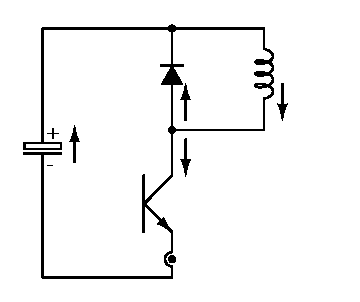
\includegraphics[scale=1.25]{schema_zakladna}\\
   % translate x=284 y=237 scale 0.28
   \putbox{1.45in}{0.99in}{1.20}{\llgic}%
   \putbox{1.45in}{1.49in}{1.20}{\llgiD}%
   \putbox{2.26in}{1.45in}{1.20}{\llgiL}%
   \putbox{0.52in}{1.14in}{1.20}{\llgiK}%
   } % close 'parbox'
   } % close 'scalebox'
   \vspace{-\baselineskip} % this is not necessary, but looks better

	\caption{Tranzistorový spínač s napäťovým medziobvodom a indukčnou záťažou}
	\label{fig:schema_zakladna}
\end{figure}

Napäťové priebehy budú snímané priamo napäťovou sondou širokopásmového osciloskopu, prúd tranzistorom bude snímaný snímačom prúdu, bližšie popísaným v stati \ref{sec:snimanie_prudu}.
Vzhľadom na vysoké frekvenčné pásmo je nutné výstup zo snímača resp. vstup do osciloskopu impedančne prispôsobiť s koaxiálnym káblom (sondy osciloskopu). %Tomuto problému je venovaný Dodatok \ref{ch:priloha_vedenie}.

V snahe o hodnoverné zmeranie priebehov charakteristických pre konkrétnu súčiastku  je nutné eliminovať vplyvy (obzvlášť tie, ktoré nemožno presne identifikovať) ostatných prvkov, ktorými sú hlavne:
\begin{itemize}
	\item kapacita obvodu do okolia (do zeme), spôsobujúca unikajúce impulzné prúdy. V prípade úniku cez tieniaci vodič koaxiálneho kábla vzniká na jeho indukčnosti a odpore úbytok, ktorý sa pripočítavá k skutočnému snímanému signálu. Kvôli obmedzeniu kapacity bude celé meracie pracovisko v dobe merania odpojené od siete - medziobvod bude tvoriť nabitá kondenzátorová batéria, osciloskop bude napájaný akumulátorom a budič monočlánkami. Prenos riadiaceho signálu z generátora je realizovaný optickým vláknom s minimálnou kapacitou.
	\item indukčnosť v slučke medziobvod - tranzistor - dioda, spôsobujúca prekmity a úbytky v priebehoch. Pre obmedzenie indukčnosti je výhodné radiť väčšie množstvo kondenzátorov v medziobvode paralelne a prepojenie s tranzistorom realizovať sendvičovým spojom.
	\item nulová dioda, deformujúca priebehy zotavovacími dejmi. Pre minimalizovanie vplyvu diody budú vyberané diody rýchlejšie od tranzistora.
\end{itemize}


Meranie bude vykonané metódou \uv{double shot}, tj. dvomi pulzmi, počas ktorých postupne narastá prúd tlmivkou. Šírka pulzov a indukčnosť tlmivky určujú veľkosť prúdu v čase zapínania a vypínania tranzistora.

\myfig{schema_pracovisko}{Usporiadanie meracieho pracoviska.}{\label{fig:schema_pracovisko}}

Usporiadanie meracieho pracoviska je schematicky znázornené na Obr. \ref{fig:schema_pracovisko}

\section{Umiestnenie meracej zeme} \label{sec:umiestnenie_meracej_zeme}
Spoločná meracia zem sónd osciloskopu musí byť realizovaná tak, aby spoločný potenciál jednotlivých pripojení zemí bol skutočne spoločný aj pri rýchlych dynamických dejoch. Navyše je prirodzená potreba, aby sa na tomto potenciále nachádzal emitor tranzistora (čipu vo vnútri púzdra). Dynamický rozdiel potenciálov galvanicky spojených bodov je spôsobovaný indukčnosťou tohto spojenia. Preto musia byť zeme sónd pripojené geometricky v zhodnom bode, a tento musí byť umiestnený čo najbližšie k emitoru čipu. Vývody púzdra ako aj zapúzdrené bondovacie dráty zďaleka nemajú zanedbateľnú indukčnosť, ako bude overené aj meraním (kapitola \ref{ch:vysledky}). Na výkonovom emitorovom prívode vznikajú veľké hodnoty $\dif{i}/\dif{t}$, čím sa jeho indukčnosť neodstrániteľne prejaví úbytkom napätia, čo je najmä v prípade súčiastok bez vyvedeného riadiaceho emitoru (nielen) z hľadiska umiestnenia meracej a v aplikáciách hlavne riadiacej zeme značne nevýhodné.


\begin{figure}[!ht]
	\centering
	% XCircuit output "priebehy_1.tex" for LaTeX input from priebehy_1.ps
\def\putbox#1#2#3#4{\makebox[0in][l]{\makebox[#1][l]{}\raisebox{\baselineskip}[0in][0in]{\raisebox{#2}[0in][0in]{\scalebox{#3}{#4}}}}}
\def\rightbox#1{\makebox[0in][r]{#1}}
\def\centbox#1{\makebox[0in]{#1}}
\def\topbox#1{\raisebox{-0.60\baselineskip}[0in][0in]{#1}}
\def\midbox#1{\raisebox{-0.20\baselineskip}[0in][0in]{#1}}
   \scalebox{0.8}{
   \normalsize
   \parbox{4.44792in}{
   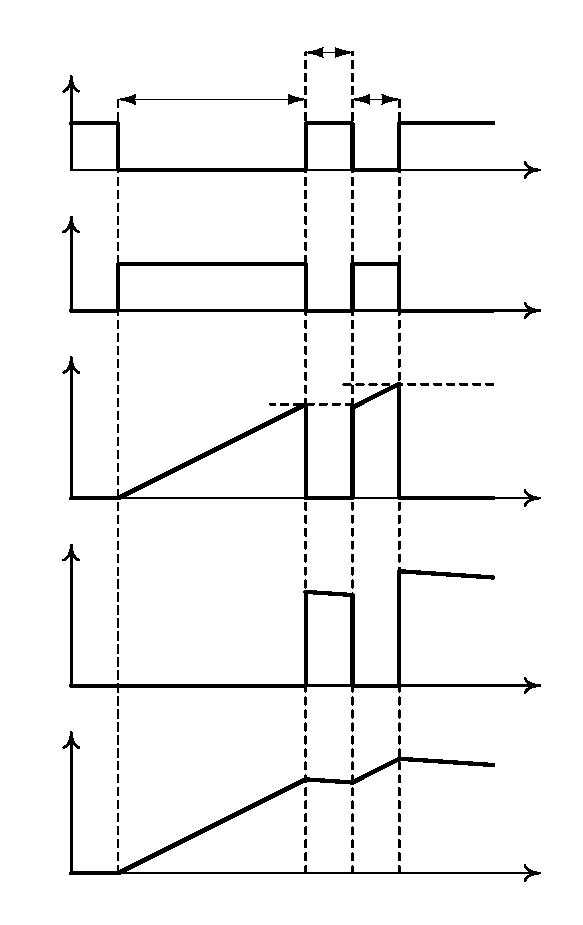
\includegraphics[scale=1.25]{priebehy_1}\\
   % translate x=314 y=1408 scale 0.30
   \putbox{4.17in}{4.78in}{1.20}{\llgt}%
   \putbox{0.06in}{5.57in}{1.20}{\llgvL}%
   \putbox{0.06in}{4.39in}{1.20}{\llgic}%
   \putbox{0.06in}{2.83in}{1.20}{\llgiD}%
   \putbox{0.06in}{1.27in}{1.20}{\llgiL}%
   \putbox{4.17in}{3.22in}{1.20}{\llgt}%
   \putbox{4.17in}{1.66in}{1.20}{\llgt}%
   \putbox{4.17in}{0.10in}{1.20}{\llgt}%
   \putbox{1.43in}{6.84in}{1.20}{\rotatebox{-360}{\llgTonj}}%
   \putbox{2.80in}{6.84in}{1.20}{\llgTond}%
   \putbox{0.06in}{6.74in}{1.20}{\llgvce}%
   \putbox{4.17in}{5.96in}{1.20}{\llgt}%
   \putbox{2.41in}{7.24in}{1.20}{\llgToffj}%
   \putbox{2.31in}{0.10in}{1.20}{\llgtj}%
   \putbox{2.71in}{0.10in}{1.20}{\llgtd}%
   \putbox{2.07in}{4.30in}{1.20}{\llgIc}%
   \putbox{3.27in}{4.47in}{1.20}{\llUmerBmax}%
   } % close 'parbox'
   } % close 'scalebox'
   \vspace{-\baselineskip} % this is not necessary, but looks better

	\caption{Principiálne priebehy pri meraní \uv{double shot} metódou.}
	\label{fig:priebehy_1}
\end{figure}

%\section{Tranzistorový spínač}


\section{Tlmivka a šírka pulzov} \label{sc:pulzy}
Šírka prvého pulzu \llgTonj na Obr. \ref{fig:priebehy_1} určuje hodnotu prúdu tlmivkou v~čase \llgtj. Pri pevne zvolenej indukčnosti tlmivky je doba \llgTonj funkciou indukčnosti, meraného prúdu \llgIc a napätia na medziobvode \llgUd podľa vzťahov:
\begin{equation}
	\llgic(t) = \frac{1}{L} \int u(t) \dif t + 0 = \frac{1}{L} \llgUd \llgt
	\label{eq:ic=(U/L)*t}
\end{equation}
Z~toho pri uvážaní $\llgIc = \llgic(\llgTonj)$:
\begin{equation}
	\llgTonj = \frac{\llgIc L}{\llgUd}
	\label{eq:Ton1=Ic*L/Ud}
\end{equation}

Indukčnosť tlmivky je nutné vypočítať pre najnepriaznivejšiu situáciu, tj. pre malý prúd a veľké napätie medziobvodu. Pre priaznivejšie prúdy a napätia stačí následne meniť dobu zapnutia tranzistora podľa (\ref{eq:Ton1=Ic*L/Ud}), s predpokladom dostatočne veľkej kapacity medziobvodu. Pre malé prúdy bude kritická veľkosť tlmivky, pre veľké prúdy kapacita medziobvodu.

Doba \llgTonj musí byť dostatočne veľká na to, aby sklon nárastu prúdu za čas spínacích dôb bol zanedbateľný. 
Voľme 
\begin{equation}
	\llgTonj = 50 \un{\mu s}.
	\label{eq:Tonj_volba_50us}
\end{equation}
a ako \uv{nepriaznivé} podmienky uvažujme $\llgIc \approx 20 \un{A}$, $\llgUd \approx 500 \un{V}$.

Podľa {\ref{eq:Ton1=Ic*L/Ud}}:
\begin{equation}
	L = \frac{\llgTonj \llgUd_{max}}{\llgIc_{min}}
	\label{eq:L=Ton1*Ud/Ic}
\end{equation}
Z čoho po dosadení vyplýva minimálna indukčnosť $\approx 1\un{mH}$.\\
Realizácia tak veľkej indukčnosti bude v podobe pomerne veľkej cievky so vzduchovou medzerou.


Počas doby vypnutia \llgToffj dochádza k~zanedbateľnej demagnetizácii tlmivky priepustným napätím nulovej diody. Hodnota \llgToffj teda nie je kritická. Dbáme len o to, aby boli na osciloskope zreteľné jednotlivé javy, preto voľme dostatočne veľkú dobu:
\begin{equation}
	\llgToffj = 10 \un{\mu s}
	\label{eq:Toff1_volba_10us}
\end{equation}

počas doby pulzu \llgTond prúd \llgic lineárne (za predpokladu zanedbateľného poklesu \llgUd) narastá nad menovitú hodnotu; jedná sa teda o~nebezpečný úsek merania a dobu \llgTond treba preto minimalizovať.

\section{Medziobvod} \label{sc:medziobvod}
Napäťový medziobvod tvorí kondenzátorová batéria, umožňujúca v~dobe merania úplné odpojenie od siete.

Prepojenie medziobvodu s~meraným spínačom je konštruované v~podobe sendvičového spoja (každá strana spoja tvorí fóliový vodič) za účelom minimalizácie indukčnosti prívodov. Malá indukčnosť je dosiahnutá malou plochou takto vytvoreného závitu vzduchovej cievky v~pomere k~dĺžke indukčnej čiary. Rozľahlosť sendvičového spoja zároveň umožňuje paralelné rozloženie kondenzátorov, čím sa eliminuje ich parazitná indukčnosť.

\subsection{Výpočet kapacity kondenzátorovej batérie} \label{ssc:vypocet_kapacity}

Účelom medziobvodu bude preakumulovanie energie do tlmivky, a to na hodnotu určenú meraným menovitým prúdom \llgIc, pri vybití nanajvýš o~zvolenú prípustnú hodnotu $\Delta U$ (na Obr. \ref{fig:priebehy_1} je pokles napätia medziobvodu zanedbaný). 

Kondenzátorom tečie vybíjací prúd iba v~dobe zapnutia tranzistora, je teda totožný s~priebehom kolektorového prúdu na Obr. \ref{fig:priebehy_1}, až na polaritu, nakoľko kondenzátor pracuje v~zdrojovom režime. Celkový náboj odobraný kondenzátoru počas jedného merania, využijúc značenie podľa Obr. \ref{fig:priebehy_1}, je teda:
\begin{equation}
	\Delta Q = \int_{(\llgTonj)} \llgiK(t) \dif t +  \int_{(\llgTond)} \llgiK(t) \dif t
	\label{eq:dQ=int_ic_dt}
\end{equation}
Keďže pokles po odmeraní zapínacieho deja v~čase \llgtj nie je podstatný a po dobu vypnutia \llgToffj k~vybíjaniu nedochádza, postačí uvažovať úsek \llgTonj. Potrebná kapacita plynie priamo z~definície kapacity a z~(\ref{eq:dQ=int_ic_dt}):
\begin{equation}
	C = \frac{\Delta Q}{\Delta U} = \frac{\llgIc \cdot \llgTonj}{2 \Delta U}
	\label{eq:C=Ic.Ton1/2dU}
\end{equation}
Keďže medziobvod má byť použiteľný pri všetkých meraniach, treba ho nadimenzovať na krajný prípad, tj. pre najnepriaznivejšie hodnoty. Dosadením najvyššej menovitej hodnoty spomedzi meraných tranzistorov $\llgIc = \llgIc_{max}$ a $\llgUd = \llgUd_{min}$ do (\ref{eq:Ton1=Ic*L/Ud}) a následne do (\ref{eq:C=Ic.Ton1/2dU}) je vyjadrená hľadaná kapacita:
\begin{equation}
	C \geq \frac{\llgIc_{max}\llgTonj_{max}}{2 \Delta U} = \frac{\llgIc_{max}^2 \cdot L}{2 \llgUd_{min}\Delta U}
	\label{eq:C}
\end{equation}
Voľba $\Delta U$:
\begin{equation}
	\Delta U = 5 \un{V}
	\label{eq:delta_U_volba}
\end{equation}
Potom pre $\llgIc_{max} = 100 \un{A}$, $\llgUd_{min} = 100 \un{V}$ a $L=1\un{mH}$ bude podľa (\ref{eq:C})
\begin{equation}
	C \geq \frac{100^2 \cdot 1\E{-3}}{2 \cdot 100 \cdot 5} = 10 \un{mF}
	\label{eq:C_vypocet}
\end{equation}

Potrebná kapacita je vytvorená kondenzátorovou batériou zo 16 paralelných výkonových polypropylénových low ESR bezindukčných kondenzátorov \cite{kondenzator-polypropylen} $40\un{\mu F}$ / $900\un{V}$ a 17 paralelne zaradených sériových dvojíc elektrolytických kondenzátorov \cite{kondenzator-elektrolyt} $1000 \un{\mu F}$ / $400\un{V}$.


\section{Snímanie prúdu} \label{sec:snimanie_prudu}

Presné snímanie kolektorového je obtiažné kvôli jeho veľkosti a rýchlosti spínania. 


\subsection{Bočník}
Najjednoduchším spôsobom snímania prúdu v prípade kedy nie je nutné galvanické oddelenie je prevodník prúdu na napätie v podobe bočníka.

Každý bočník má však parazitnú indukčnosť, ktorá vytvára s jeho odporom hornopriepustný derivačný článok. To je jeho hlavnou a podstatnou nevýhodou. Preto sa zvykne signál z bočníka frekvenčne kompenzovať zaradením RC-článku. V prípade takého merania, aké je predmetom tejto práce, by kompenzácia RC-článkom zrejme bola príliš dobrodružná, môžeme si však dovoliť väčšie hodnoty odporu vedúce k zanedbateľnému vplyvu parazitnej indukčnosti bočníka, hoci za cenu nezanedbateľného ohmického úbytku, ktorý sa z dôvodu pripojenia riadiacej zeme podľa Obr. \ref{fig:schema_pracovisko} premietne do snímaného priebehu kolektorového napätia. Tento úbytok je ale spätne rekonštruovateľný (zo známosti kolektorového prúdu).

Konštrukčne je vhodné realizovať bočník paralelným spojením viacerých SMD rezistorov, čím sa dosiahne zmenšená indukčnosť v porovnaní z indukčnosťou jediného rezistora.
Toto riešenie sa ukázalo využiteľnejšie, než koaxiálny bočník, ktorý býva konštruovaný o malých hodnotách odporu.


\subsection{Prúdový transformátor}
V prípade nutnosti galvanického oddelenia je možnosť použiť transformátor prúdu. Jeho výstupom je prúdový signál, takže je znovu nutné použiť bočník.

Transformátor síce z~princípu neumožňuje prenos jednopolaritného prúdu, ale pre snímanie prechodových dejov jeho použitie má zmysel. Nemožnosť jednosmerného prenosu ide v~tomto prípade do úzadia, pretože účelom je snímať iba dva pulzy - \llgic na Obr. \ref{fig:priebehy_1}. Návrh sýtenia jadra vychádza z~totožného obrázku a z~náhradného modelu (prúdového) transformátora na Obr. \ref{fig:prudove_trafo_model}, veľmi zreteľne odvodeného vedúcim tejto práce v~\cite{patocka:kniha}.
\begin{figure}[!ht]
	\centering
	% XCircuit output "prudove_trafo_model.tex" for LaTeX input from prudove_trafo_model.ps
\def\putbox#1#2#3#4{\makebox[0in][l]{\makebox[#1][l]{}\raisebox{\baselineskip}[0in][0in]{\raisebox{#2}[0in][0in]{\scalebox{#3}{#4}}}}}
\def\rightbox#1{\makebox[0in][r]{#1}}
\def\centbox#1{\makebox[0in]{#1}}
\def\topbox#1{\raisebox{-0.60\baselineskip}[0in][0in]{#1}}
\def\midbox#1{\raisebox{-0.20\baselineskip}[0in][0in]{#1}}
   \scalebox{0.8}{
   \normalsize
   \parbox{4.55729in}{
   
\includegraphics[scale=1.25]{prudove_trafo_model}\\
   % translate x=231 y=245 scale 0.30
   \putbox{1.19in}{0.26in}{1.20}{\llgud}%
   \putbox{1.36in}{0.85in}{1.20}{\llgij}%
   \putbox{0.52in}{0.51in}{1.20}{\llgudb}%
   \putbox{0.11in}{1.35in}{1.20}{\llgij}%
   \putbox{1.86in}{1.35in}{1.20}{\llgidk}%
   \putbox{2.52in}{0.85in}{1.20}{\rotatebox{-360}{\llgimag}}%
   \putbox{2.90in}{0.51in}{1.20}{\llgud}%
   \putbox{3.27in}{1.26in}{1.20}{\llgRcu}%
   \putbox{4.11in}{0.51in}{1.20}{\rotatebox{-360}{\llgRb}}%
   } % close 'parbox'
   } % close 'scalebox'
   \vspace{-\baselineskip} % this is not necessary, but looks better

	\caption{Obvodový model transformátora (prúdu).}
	\label{fig:prudove_trafo_model}
\end{figure}
S predpokladom správneho návrhu možno uvažovať:
\begin{equation}
	\llgimag << i_2 \implies \llgud = i_2 \cdot R
	\label{u2=i2*R}
\end{equation}

Potom tok v jadre bude (s nulovým počiatočným tokom):
\begin{equation}
    \Psi(t) = \int R_2 \cdot \frac{\llgUd}{L} \frac{1}{N_2} \cdot t \dif t = \frac{R_2 \llgUd}{2 L N_2} t^2
	\label{eq:Psi_t}
\end{equation}
$L$ je indukčnosť záťažnej tlmivky (určujúcej spolu s napätím medziobvodu smernicu lineárneho nárastu prúdu).

Pre sýtenie jadra možno písať:
\begin{equation}
	\Psi_{max} = \frac{R_2 \llgUd}{2 L N_2} (\llgTonj + \llgTond)^2 = N_2 B_{max} S_{Fe}
	\label{Psi_max}
\end{equation}

Z toho plynie vzťah na kontrolu sýtenia pri zvolenom jadre a počte závitov:
\begin{equation}
    N_2 \geq \sqrt{\frac{R_2 \llgUd}{2 B_{max} S_{Fe} L} (\llgTonj+\llgTond)^2}
	\label{eq_N2_fTon1Ton2}
\end{equation}

Pri zanedbaní \llgTond oproti \llgTonj a pri pevnej indukčnosti (\llgTonj je funkciou indukčnosti):
\begin{equation}
    N_2 \geq \sqrt{\frac{R_2 L I_{C,max}^2}{2 B_{max}S_{Fe}\llgUd_{min}}}
	\label{eq:N2_fIcUd}
\end{equation}






\subsection{Rogowského cievka}
Výhodou Rogowského cievky je skutočnosť, že na snímanie osciloskopom nie je potrebný bočník. Problémy s parazitnou indukčnosťou preto odpadajú.

Nevýhodou je nutnosť integrovať výstupný signál, aby sa rekonštruoval vstupný prúd. Pri tak vysokom frekvenčnom pásme, aké je nevyhnutné na snímanie prepínacích dejov prichádza v úvahu jedine pasívny integrátor. 
Výstupom z Rogowského cievky je slabý signál veľmi náchylný na rušenie. Tento spôsob snímania sa neosvedčil.


\section{Budič bázy resp. hradla} \label{sc:budič}
Budič (Dodatok \ref{ch:priloha_schemy}, stať \ref{sec:append_budic}) vychádza zo schémy uvedenej v \cite{patocka-skripta-3} pre budič bipolárneho výkonového tranzistora. Je schopný dodávať do bázy trvalý prúd obmedzený odporom $R5$ na cca $2\un{A}$, špičkovo $5\un{A}$, a pri vypínaní špičkovo aj $-8\un{A}$. Je modifikovaný tak, aby sa dal prepojiť skratovacími prepojkami do režimu budenia unipolárnych tranzistorov. Horná i spodná napäťová úroveň je nastaviteľná regulátorom napätia v napájacom obvode (stať \ref{sec:append_nap}) napájanom monočlánkami.


\section{Generátor impulzov} \label{sec:generator}
Dva spínacie pulzy sú generované analógovým generátorom, odolným proti rušeniu, pripraveným špeciálne na tento účel. Prvý zapínací pulz generuje monostabilný obvod s nastaviteľnou dobou kyvu ($T_{on,1}$ na Obr. \ref{fig:priebehy_1}), triggrovaný tlačítkovým spínačom. Na jeho vypínaciu hranu je následne triggrovaný druhý monostabilný obvod, ktorého doba kyvu určuje dobu vypnutia tranzistora ($T_{off,1}$). Na jeho vypínaciu hranu je triggrovaný tretí monostabilný obdov, určujúci dobu $T_{on,2}$. Štvrtý monostabilný obvod  s dobou kyvu rádovo $10\un{s}$ (triggrovaný s malým oneskorením spolu s prvým pulzom) zablokuje vstup kaskády generujúcej pulzy, kvôli ochrane pred náhodným opätovným zopnutím.

Schéma zapojenia a DPS sú priložené v Dodatku \ref{ch:priloha_schemy}, stať \ref{sec:append_gen}.


\chapter{Časovo premenná vodivosť $g_{CE}$} \label{ch:gce}

\lettrine{A}{ko} bolo naznačené v úvode, s odkazom na článok \cite{valsa-patocka-petru}, spínací tranzistor možno jednoduchým spôsobom fenomenologicky \uv{dvojpólovo} modelovať ako časovo premennú vodivosť medzi kolektorom a emitorom. Myšlienka neskokovej zmeny tranzistora z nevodivého stavu do vodivého a naopak je pomerne prirodzená, jej dôsledné rozvinutie je však mimoriadne užitočné, a to nielen pre jednoduchosť modelu, ale aj pre prehľadnú analýzu celého tranzistorového spínača so záťažou (Obr. \ref{fig:schema_zakladna_ch_gce}) za predpokladu, že časový priebeh vodivosti $g_{CE}(t)$ nezávisí na kolektorovom obvode. 

\myfigtex{obr/schema_zakladna}{Tranzistorový spínač}{\label{fig:schema_zakladna_ch_gce}}
\myfigtex{obr/plots/simulacia_zakladna_300V100V}{Predstava vodivosti $g_{CE}(t)$ behom vypínacieho deja.}{\label{fig:simulacia_zakladna_300V100V}}

Demonštrovať to možno na príklade analýzy spínania indukčnej záťaže, zabezpečujúcej po krátku dobu zapnutia / vypnutia konštantný prúd.  Z modelu je evidentné, že zlom v priebehoch napätia aj prúdu (na Obr. \ref{fig:simulacia_zakladna_300V100V} je zobrazený príklad vypínacieho deja) nie je priamo daný tranzistorom, ale súčinnosťou celého obvodu, teda prakticky nulovou diodou, napäťovým a prúdovým zdrojom (medziobvod a tlmivka). Je samozrejmé, že časová poloha tohto zlomu (resp. rýchlosť deja) je určená vlastnosťami tranzistora, nijako však nesúvisí s nejakým \uv{zlomom} v dejoch vo vnútri tranzistora. Dochádza k nemu v momente, kedy je nulová dioda prepólovaná do priepustného smeru (napätie na anóde presiahne napätie na katóde). Do tohto momentu bol konštantný prúd záťaže $i_L$ nútený tiecť klesajúcou vodivosťou $g_{CE}$ spôsobujúcou zväčšujúci sa úbytok $u_{CE}$. Od okamihu prepólovania diody je na kolektore udržované konštantné napätie medziobvodu, nezávisle na veľkosti prúdu $i_D(t)$. Vodivosť $g_{CE}$ naďalej klesá, čím postupne núti čoraz väčší podiel konštantného prúdu záťaže odtekať cestou cez diodu, až po ustálený stav, kedy je tranzistor zavretý.


Ďalej z tohto jednoduchého modelu plynie, že doby známe ako $t_d$ (\textit{delay time}) a $t_f$ (\textit{fall time}), ktoré sa menia v závislosti na veľkosti spínaného napätia, sú spolu zviazané vzťahom $t_d + t_f = t_{off}$, kde $t_{off}$ je celková vypínacia doba, ktorá je nezávislá na napätí (Obr. \ref{fig:simulacia_zakladna_300V100V}). Závislá je na spôsobe budenia tranzistora, teplote či veľkosti spínaného prúdu (ako bude pozorované aj v meraniach prezentovaných v kapitole \ref{ch:vysledky}), ktoré ovplyvňujú tvar krivky časového priebehu $g_{CE}(t)$.

Autori článku \cite{valsa-patocka-petru} v čase jeho vzniku pozorovali pri množstve meraní bipolárneho tranzistora za rozličných podmienok tvar krivky $g_{CE}(t) = \frac{i_C(t)}{u_{CE}(t)}$ ako hladký, tvarovo typicky vystihnutý na analyzovanom Obr. \ref{fig:simulacia_zakladna_300V100V}. Nakoľko je jej priebeh hladký\footnote{Každopádne platí predchádzajúca analýza a možno tvrdiť minimálne toľko, že v okamihu \uv{zlomu} v priebehoch je priebeh krivky hladký}, najmä pri moderných rýchlych unipolárnych súčiastkach, je presne analyticky vyjadrovať nemožné; podstatná je myšlienka, že vypínací i zapínací dej možno analyzovať ako \uv{číru} vodivosť vyjadriteľnú Ohmovým zákonom ako $\frac{i(t)}{u(t)}$ a prehnutý tvar priebehov nie je teda daný nijakými zotrvačnými javmi, ako napr. kapacitou.

Nakoniec, v prípade, že by to neplatilo, neplatila by ani všeobecne zaužívaná \uv{definícia} stratového výkonu počas spínania v podobe $p(t)~=~u_{CE}(t)~\cdot~i_C(t)$.



\section{Stručná analýza spínacích dejov v tranzistoroch} \label{sec:analyza}



Bez toho, aby sme zachádzali do zdĺhavej kvantitatívnej analýzy fyzikálnych dejov v tranzistore je možné aspoň v základných črtách naznačiť charakter týchto dejov.

\subsection{Bipolárny tranzistor}

Vo vysokonapäťových súčiastkach je nutné na udržanie záverného napätia (vyprázdnenou oblasťou prechodu) konštruovať slabo dotovanú tzv. driftovú oblasť. Býva dotovaná prímesami typu N, oblasť typu P je optimalizovaná naopak pre dobré vedenie prúdu v zapnutom stave.
Zjednodušená jednorozmerná štruktúra tranzistora (reálne podobná prierezu pod emitorom) je na Obr. \ref{fig:BJT_struktura_1D}.

\myfigtex{obr/BJT_struktura_1D}{Jednorozmerná štruktúra výkonového BJT.}{\label{fig:BJT_struktura_1D}}

V dôsledku odporu N-drift vrstvy vzniká vo výstupných charakteristikách tzv. kvázi-saturačná oblasť - Obr. \ref{fig:BJT_iv}, ktorá znázorňuje zvýšený úbytok $U_{CE,sat}$ v zapnutom stave.

\myfigtex{obr/BJT_iv}{Výstupné charakteristiky výkonového BJT.}{\label{fig:BJT_iv}}

%\subsection{Zapnutý stav - saturačná oblasť}

Tranzistor pracuje v saturačnej oblasti v situácii, keď oba prechody, báza-emitor aj báza-kolektor, sú pólované priepustne. Prúdové zosilenie tranzistora je menšie než v aktívnej oblasti (\textit{forward-active mode}). Kolektorový prúd je totiž určený difúziou elektrónov v oblasti bázy, pričom difúzia akéhokoľvek druhu je úmerná zmene koncentrácie na jednotku dĺžky, teda $\dxdt{n}{x}$. Priebeh koncentrácie nosičov v báze možno približne určiť superpozíciou koncentrácií v režime aktívnom (\textit{forward-active}) a inverznom aktívnom (\textit{reverse-active}), ktoré sa vyznačujú tým, že jeden z prechodov je v priepustnom a druhý v závernom stave (tj. s nulovou koncentráciou minoritných nosičov na rozhraní bázy a danej oblasti) - Obr. \ref{fig:BJT_sat_koncentracie_baza}. Výsledkom ich superpozície je síce väčšie množstvo náboja v báze, ale s menším gradientom, a na dosiahnutie rovnakého kolektorového prúdu je nutné tranzistor budiť väčším bázovým prúdom (prebudiť). 

\myfigtex{obr/BJT_sat_koncentracie_baza}{Koncentrácia náboja v báze v saturačnom režime BJT ako superpozícia koncentrácii aktívneho a inverzného režimu. Označenia \uv{F} a \uv{R} znamenajú priepustné (\textit{forward}) a záverné (\textit{reverse}) pôlovanie daného prechodu.}{\label{fig:BJT_sat_koncentracie_baza}}

Dôsledkom je však zároveň väčšia koncentrácia dier v oblasti kolektora, čím sa pri uvažovaní zachovania nábojovej neutrality zvyšuje vodivosť tejto oblasti (\textit{conductivity modulation}, \cite{shockley}) a znižuje napätie na hodnotu $U_{CE,sat}$.

Z hľadiska zamerania tejto práce je dôležitý poznatok, že napätie $u_{CE}$ je určené podstatnou mierou vodivosťou kolektorovej oblasti, a tá je modulovateľná  injekciou dier.

Medzi saturačným a aktívnym režimom je nutný prechodný stav, ktorému sa hovorí - ako bolo spomenuté - kvázi-saturačný režim, teda stav, kedy už dochádza k k modulácii vodivosti driftovej oblasti, ale šírka modulovanej oblasti je menšia než celá šírka oblasti. Pre ilustráciu týchto troch režimov sú na Obr. \ref{fig:BJT_koncentracie_vsetky_rezimy} zobrazené približné koncentrácie voľných nosičov v tranzistore v jednotlivých režimoch pri rovnakom kolektorovom prúde $I_C$. Odvodenie lineárneho priebehu koncentrácie v driftovej oblasti je možné (napr.\cite{lutz}), nejedná sa iba o odhad.

\myfigtex{obr/BJT_koncentracie_vsetky_rezimy}{Tri režimy BJT pri rovnakom prúde $I_C$. Označenia \uv{F} a \uv{R} znamenajú priepustné (\textit{forward}) a záverné (\textit{reverse}) pôlovanie daného prechodu.}{\label{fig:BJT_koncentracie_vsetky_rezimy}}

Hromadenie náboja v driftovej oblasti je pomerne zdĺhavé (čo zodpovedá \uv{priehybu} časového priebehu vodivosti $g_{CE}$ a teda spomaleniu prudkosti zapínacieho deja v jeho konečnej fáze (trajektória pracovného bodu na Obr. \ref{fig:BJT_iv_indukc} vstupuje do kvázisaturačnej oblasti v záverečnej fáze deja) a podobne tak pomalé je i vyprázdňovanie náboja z oblasti pri vypínaní, čomu zodpovedá spomalenie prudkosti vypínacieho deja v jeho počiatočných fázach (aby bolo možné záverné pólovanie prechodu báza-kolektor, musí byť dosiahnutá koncentrácia nosičov na tomto prechode nulová).
\myfigtex{obr/BJT_iv_indukc}{Trajektória pracovného bodu počas spínania indukčnej záťaže.}{\label{fig:BJT_iv_indukc}}

Nakoľko je reč o minoritných dierach v oblasti kolektoru (typu N), je zrejmé, že hromadenie či vyprázdňovanie je hlavnou mierou určené dierovým prúdom bázy (typ P). Veľkosťou bázového prúdu je teda možné značne urýchliť spínacie deje. Podobným mechanizmom, ako hromadenie resp. odsávanie náboja z kolektorovej oblasti je nutné nahromadiť resp. vyprázdniť náboj (minoritné elektróny) aj z bázy; aj tu platí, že bázovým prúdom je možné dej značne urýchliť.

V aktívnej oblast tranzistora je možná analýza pomocou \textit{charge control} princípov známych z analýzy signálových tranzistorov.

V reálnej súčiastke a aplikácii je celá situácia komplikovanejšia. Geometria tranzistora je nie je zhodná s jednorozmerným modelom, skutočná šírka bázy sa počas dejov môže meniť, rekombinácia je prítomná aj v báze (i keď nie dominantná) atď. Nebude preto prekvapujúce, že v časovom priebehu vodivosti $g_{CE}$ nie sú rozoznateľné nejaké ostré zmeny, naopak bude pomerne presne aproximovateľná hladkou krivkou.



\subsection{Unipolárne tranzistory}
U unipolárnych súčiastkach je riadiaca elektróda oddelená od emitora (resp. \textit{source}) izolačnou vrstvou oxidu. Táto dielektrická vrstva spolu s vodivým hradlom a emitorom vytvára kapacitu $C_{GE}$ (resp. $C_{GS}$. Pre vytvorenie inverznej vrstvy (kanálu) v súčiastke - tj. pre zapnutie tranzistora - je nutné nabíť  kapacitu $C_{GS}$ na hodnotu prahového napätia (u výkonových tranzistorov okolo $5\un{V}$. Po vytvorení vodivého kanálu začne narastať prúd tranzistorom, v závislosti na ešte stále narastajúcom napätí $u_{GS}$. Prepočítavacím pomerom je transkonduktancia unipolárnej súčiastky. Po tom, ako prúd dosiahne plnú hodnotu prúdu záťaže, ostáva konštantný, a tak je (prepočítané cez transkonduktanciu) konštantné aj napätie $u_{GS}$ - vzniká typické plató v priebehu $u_{GS}$. Ďalšia prítomná kapacita - $C_{GD}$ je vybíjaná prúdom do hradla a tým klesá aj napätie $u_{DS}$ (napätie $u_{GS}$ je v tejto fáze konštantné, čo značí, že do kapacity $C_{GS}$ už nevteká nijaký prúd). Napätie $u_{GS}$ sa nakoniec ustáli na hodnote kladného budiaceho napätia (obe kapacity sa nabijú na ustálené hodnoty).

Veľmi obdobne prebieha tiež vypínací dej.

Z popisu je zrejmé, že rýchlosť  spínacích dejov (a teda tvar časového priebehu vodivosti $g_{CE}$) je silne závislá na veľkosti nabíjacieho odporu $R_G$. 

U unipolárnych tranzistorov (MOSFET) nedochádza k nijakému hromadeniu náboja alebo rekombinácii, preto sú tieto súčiastky omnoho rýchlejšie, než bipolárne (avšak za cenu, že v nutne prítomnej driftovej oblasti nie je možné modulovať vodivosť injektovaním minoritných nosičov - charakteristika tranzistoru MOSFET v zapnutom stave je $R_{DS,on}$, a nie saturačné napätie nezávislé na prúde).

Spínacie deje v tranzistoroch IGBT sú kombináciou unipolárnych (rýchle otvorenie kanálu) a bipolárnych dejov (pomalé hromadenie resp. rekombinácia minoritných nosičov (nie je tu prítomný ani odsávací bázový prúd)). Prakticky je možnosť ovplyvniť rýchlosť spínania IGBT jedine veľkosťou nabíjacieho prúdu $R_G$.


\chapter{Vplyv parazitných prvkov na merateľné priebehy} \label{ch:parazity}

\lettrine{P}{od} predpokladom vysloveným v kapitole \ref{ch:gce}, totiž že časový priebeh $g_{CE}(t)$ je pri zachovaných podmienkách ako spôsob budenia či veľkosť prúdu záťaže nezávislý na konkrétnom prevedení kolektorového obvodu, je možné priamočiaro analyzovať vplyv parazitným prvkov v obvode.
Niektoré parazitné vplyvy sú jednoducho overiteľné meraním, a tieto sú viac menej vo všeobecnom povedomí technikov v tejto oblasti, niektoré je naopak overiť či kvantifikovať pomerne obtiažné - keďže deformujú nasnímané priebehy do podoby veľmi nápadne podobnej priebehom bezparazitným, ako bude ukázané v nasledujúcich statiach. Keď vylúčime nesprávny spôsob snímania priebehov (ako napr. zanedbávanie indukčností spojov, vývodov, atď.) jedná sa najmä o parazity samotnej zapúzdrenej súčiastky, nakoľko pri praktických meraniach prístup dovnútra púzdra nie je možný. Nepríjemnosťou je práve podobnosť s priebehmi bezparazitnými.

V tejto kapitole budú ukázané priebehy s pomerne prehnanými hodnotami parazitných prvkov, a to vždy práve jedného, aby boli presne rozlíšené jednotlivé vplyvy, i keď v reálnej situácii by bol ich účinok kombinovaný. Uvedené obrázky možno tak použiť ako rýchlu referenciu pri analyzovaní skutočných nameraných priebehov a odhaľovaní parazitných vplyvov.


\section{Jednotlivé prípady}


\subsection{Indukčnosť sľučky medziobvod - tranzistor - dioda}
Vplyv na priebehy je znázornený na Obr. \ref{fig:sim_L3}.
\myfigschplotplottex{obr/schema_sim_L3ekvL4}{obr/plots/sim_off_L3}{obr/plots/sim_on_L3}{Vplyv parazitnej indukčnosti slučky medziobvod - tranzistor - dioda na vypínací (hore) a zapínací (dole) dej.}{\label{fig:sim_L3}}

Indukčnosť medziobvodu, schématicky indukčnosť slučky medziobvod - tranzistor - dioda, je aplikačne veľmi typickým parazitným javom. Prejavuje sa pri vypínaní typickým prekmitom kolektorového napätia, pri zapínaní zase indukčným úbytkom. Dôvodom prekmitu / podkmitu je rýchla zmena prúdu pretekajúceho indukčnosťou. Z pohľadu meraných priebehov nezáleží na tom, či je indukčnosť dominantná pred alebo za uzlom pripojenia záťaže (Obr. \ref{fig:sim_L3} hore). Smer prúdu v oboch prípadoch je síce opačný, ale opačné je aj znamienko jeho časovej derivácie (kým jedným smerom narastá, druhým klesá).
Pri menšom úsilí je tento vplyv jednoducho merateľný, pri väčšom úsilí je odstraniteľný (kapitola \ref{ch:meranie}).


\subsection{Indukčnosť medzi meracími bodmi}
Vplyv na priebehy je znázornený na Obr. \ref{fig:sim_L2}.
\myfigschplotplottex{obr/schema_sim_L1ekvL2}{obr/plots/sim_off_L2}{obr/plots/sim_on_L2}{Vplyv parazitnej indukčnosti medzi meracími bodmi na vypínací (hore) a zapínací (dole) dej.}{\label{fig:sim_L2}}
Prakticky sa jedná o indukčnosť vodivého úseku medzi meracími bodmi, teda indukčnosť vývodov tranzistorových elektród. V skutočnosti ide o ten istý jav, ako v predchadzajúcom prípade, ale je \uv{nepozorovaný}, keďže napätie v meracom bode je držané nulovou diodou. To však neznamená, že prekmit pri zapínaní nie je prítomný ani na tranzistore.
Obmedzenie indukčnosti je možné zabezpečením čo najkratších vývodov tranzistora a čo najbližším umiestnením meracích bodov k čipu. 

K bondovacím drátom vo vnútri púzdra prístu nie je možný, takže ich indukčnosť takmer nie  je možné identifikovať. Zdeformovavý trav priebehov je  prakticky nerozoznateľný od bezparazitného priebehu (pokiaľ bezparazitné meranie nie je k dispozícii), keďže k prepólovaniu diody (zlom v priebehoch) dochádza pri vypínaní v rovnakom bode, ako bez prítomnosti indukčnosti, a pri zapínaní zasa dôjde k prepólovaniu  pri plnom napätí (bez viditeľného úbytku).

Inými slovami, úbytok na indukčnosti, ktorý síce nie je v meracom bode pozorovaný, spôsobí pri zachovanej vodivosti $g_{CE}$ zníženie prúdu $i=g_{CE} u_{CE}$ a tým pádom časový posun okamihu prepólovania diody, presne tak, ako v prípade merateľného podkmitu, avšak merané napätie je skreslené indukčnosťou do podoby pripomínajúcej zlom v bezparazitných priebehoch - zmena prúdu je od toho momentu nulová a tak napätie na indukčnosti skokovo klesá na nulovú hodnotu (Obr. \ref{fig:sim_L2} dole).


\subsection{Kapacita záťaže}
Vplyv na priebehy je znázornený na Obr. \ref{fig:sim_C5}.
\myfigschplotplottex{obr/schema_sim_C1ekvC5}{obr/plots/sim_off_C5}{obr/plots/sim_on_C5}{Vplyv kapacity záťaže (paralelenej kapacity) na vypínací a zapínací dej.}{\label{fig:sim_C5}}

Z pohľadu merania je jedno, či je kapacita \uv{pripojená} paralelne k záťaži, alebo k tranzistoru (v jednom prípade sa nabíja, av druhom vybíja, ale výsledný efekt je v prípade lineárnej kapacity rovnaký). 

Ide v podstate o prípad známy z čias bipolárnych tranzistorov ako odľahčenie vypínacieho deja. Na prudkú zmenu napätia reaguje kapacita nabíjacím / vybíjacím prúdom, a keďže je zapojená paralelne k prvku, ktorý vedie prúd, jeho prúd sa zníži tak, aby ich súčet zodpovedal prúdu záťaže. v okamihu prepólovania nulovej diody sa stáva napätie $u_{CE}$ konštantným a kapacitný prúd je ďalej preto nulový (kapacita ostáva nabitá na aktuálnu hodnotu až do zapínacieho deja).

Pri zapínacom deji je naopak prítomný prekmit v priebehu prúdu $i_C$.

Prakticky je tento prípad typicky spôsobený parazitnou kapacitou záťaže (vinutia), alebo nulovej diody (tej kapacita je ale napäťovo závislá, čomu sa bližšie venuje stať \ref{sec:varikap}).

\myfigschplotplottex{obr/schema_sim_C5nelin}{obr/plots/sim_off_C5nelin}{}{Vplyv napäťovo závislej kapacity varikapu na vypínací a zapínací dej.}{\label{fig:sim_C5nelin}}


\subsection{Kapacita tranzistora $C_{CE}$} 
\myfigschplotplottex{obr/schema_sim_C2}{obr/plots/sim_off_C2}{obr/plots/sim_on_C2}{Vplyv vnútornej kapacity $C_{CE}$ súčiastky na vypínací a zapínací dej.}{\label{fig:sim_C2}}
Inú situáciu predstavuje \uv{vnútorná} výstupná kapacita zapúzdreného tranzistora, teda kapacita medzi kolektorom a emitorom. Odlišnosť spočíva v tom, že neexistuje možnosť, ako separovane merať prúd vodivosťou a paralelnou kapacitou. Ich súčet nutne zodpovedá prúdu záťaže, takže nie je možné pozorovať (pri vypínaní) zníženie prúdu tranzistorom, i keď v skutočnosti prítomné je, a znovu tak, ako v predchádzajúcom prípade spôsobuje tiež zníženie okamžitého napätia $u_{CE} = \frac{i_C}{g_{CE}}$ na nezmenenej vodivosti. Zlom vo vypínacom deji sa časovo posunie, ale tvarovo sa priebehy ponášajú na priebehy bezpartitné - v okamihu kedy sa napätie stáva konštantným skokovo zaniká prúd diodou - Obr. \ref{fig:sim_L2}.

Prakticky možno hovoriť buď o rôznych parazitných kapacitách izolovaných častí v púzdre (najmä u výkonových moduloch (\cite{lutz}, \cite{khanna}), v jednom diskrétnom púzdre vplyv ukazuje byť zanedbateľným) a o kapacite samotného polovodičového prechodu (stať \ref{sec:varikap}).

%\myfigschplotplottex{obr/schema_sim_C2nelin}{obr/plots/sim_off_C2nelin}{}{<++>}{\label{fig:sim_C2nelin}}




\section{Kapacita záverne pólovaného prechodu PN} \label{sec:varikap}
Samotný PN prechod báza-kolektor či prechod nulovej diody vykazuje v závernom smere\footnote{behom spínacích dejov je prechod báza kolektor aj prechod nulovej diody jednak väčšinu času pólovaný záverne, jednak v priepustnom smere všeobecne nie sú umožnené veľké zmeny napätia} kapacitu. Nejedná sa o klasický platňový kondenzátor vyplnený dielektrikom, ale výsledný efekt nabíjacieho resp. vybíjacieho prúdu pri zmene priloženého napätia je obdobný. Tento prúd nie je prúdom nosičov urýchľovaných elektrickým poľom v polovodiči, čiže drift, pojem úzko spätý s predstavou vodivosti. Jeho pôvodom je rozširovanie vyprázdnenej oblasti priestorového náboja (nabitých donorov, prípadne akceptorov) a teda vyprázdňovanie pôvodne neutrálnej oblasti od nosičov náboja pri zväčšovaní záverného napätia a naopak.

\myfigtex{obr/pn_kapacita}{Ku kapacite PN prechodu}{\label{fig:pn_kapacita}}

Matematicky možno slovne popísanú situáciu vyjadriť kratšie; nasledovne:
\begin{equation}
    \dxdt{U}{t} \rightarrow \dxdt{W}{t} \approx \dxdt{Q}{t} = i(t)
    \label{eq:dU->dW->dQ}
\end{equation}

Pri predpoklade $p^+n$ prechodu a pre jednoduchosť využijúc tzv. \textit{depletičnú aproximáciu} je množstvo náboja chýbajúce k neutralizácii náboja ionov vo vyprázdnenej oblasti úmerné šírke tejto oblasti:
\begin{equation}
    Q = q N_D W_D
    \label{eq:Q--qNW}
\end{equation}
kde $q$ je náboj jedného nosiča, $N_D$ je koncentrácia donorovej prímesi.
Preto:
\begin{equation}
    i(t) = \dxdt{Q}{t} = q N_D \dxdt{W(U(t))}{t} = \underbrace{q N_D \dxdt{W}{U}}_{C(U)}\dxdt{U}{t} 
    \label{eq:dQdt--qN.dWdU.dUdt}
\end{equation}
čo je známa forma rovnice prúdu kondenzátora.


Makroskopická šírka vyprázdnenej (depletičnej) vrstvy $W_D$ (Obr. \ref{fig:pn_kapacita}) je závislá na absolútnej veľkosti záverného napätia (na offsete), preto je kapacita (spôsobená malými zmenami $dW$ resp. $dU$ v pomere k $W_D$ resp. $U_0$) prechodu tiež silne napäťovo závislá.
Keďže závislosť šírky vyprázdnenej oblasti - úmernej množstvu vyprázdneného náboja - od napätia je nelineárna, je nelineárnou aj napäťová závislosť kapacity. 
Pre vyjadrenie tejto závislosti sa nezaobídeme bez vzťahu známeho z fyziky polovodičov (\cite{lutz}, \cite{baliga}) - pre najjednoduchší prípad skokového prechodu:
\begin{equation}
    W_D = \sqrt{\frac{2 \epsilon (U_{bi} + U)}{q N_D}}
    \label{eq:Wd--fU}
\end{equation}
kde $\epsilon$ je permitivita polovodiča, $U_{bi}$ je vnútorné napätie prechodu (\textit{built-in voltage}) a $U$ je aplikované záverné napätie. Pre priepustné pólovanie vzťah neplatí.

Derivovaním (\ref{eq:Wd--fU}) podľa napätia a dosadením do (\ref{eq:dQdt--qN.dWdU.dUdt}) vznikne:
\begin{equation}
    i(t) = \underbrace{\sqrt{\frac{\epsilon q N_D}{U_{bi} + U}}}_{C(U)} \cdot \dxdt{U}{t}
    \label{eq:i--C(U)dUdt}
\end{equation}
Z toho pre jednoduchosť možno vyjadriť približný vzťah:
\begin{equation}
    C(U) = C_0 \frac{1}{\sqrt{1+U}}
    \label{eq:C(U)=C0.1/sqrt(1+U)}
\end{equation}

\myfigtex{obr/varikap_CV_krivka}{$C-V$ krivka varikapu.}{\label{fig:varikap_CV_krivka}}

Graficky je takáto $C-V$ krivka vynesená na Obr. \ref{fig:varikap_CV_krivka}. Jedná sa o závislosť typickú pre varikap.


\subsection{Možný vplyv kapacity PN-prechodu na priebehy}
Z podstaty spínacích priebehov pri indukčnej záťaži plynie, že k veľkým hodnotám $\dxdt{u}{t}$ na tranzistore dochádza pri veľkej absolútnej hodnote $u_CE$, kedy je kapacita varikapu malá. Pri malých hodnotách napätia sú malé i hodnoty $\dxdt{u}{t}$ a napriek prípadnej veľkej hodnote kapacity prechodu je už jej účinok takmer nulový.

V prípade kapacity nulovej diody je situácia opačná. I tu je však celkový vplyv menší, než u napäťovo nezávislej kapacity (pre ilustráciu je možné porovnať obrázky vypínacích priebehov ovplyvnených napäťovo nezávislou kapacitou a napäťovo závislou podľa (\ref{eq:C(U)=C0.1/sqrt(1+U)}) s rovnakou hodnotou $C_0$ - Obr. \ref{fig:sim_C5} a Obr. \ref{fig:sim_C5nelin}.

Prakticky znateľne výraznejším sa ukazuje byť vplyv kapacity záťaže, a ten je pri meraniach možné obmedziť.





\chapter{Aproximácia vodivosti $g_{CE}$ analytickou funkciou} \label{ch:krivka}

\lettrine{B}{udeme} hľadať interpolačnú funkciu $g(t)$ vyhovujúcu predpisu:
\begin{equation}
	\begin{array}{c | c c c}
		t & t_0 & t_1 & t_2 \\
		\hline
		g(t) & G_0 & G_1 & G_2
	\end{array}
	\label{eq:tab_predpis_t012}
\end{equation}

\begin{figure}[ht!]
	\centering
	% XCircuit output "krivka_vyp_t012.tex" for LaTeX input from krivka_vyp_t012.ps
\def\putbox#1#2#3#4{\makebox[0in][l]{\makebox[#1][l]{}\raisebox{\baselineskip}[0in][0in]{\raisebox{#2}[0in][0in]{\scalebox{#3}{#4}}}}}
\def\rightbox#1{\makebox[0in][r]{#1}}
\def\centbox#1{\makebox[0in]{#1}}
\def\topbox#1{\raisebox{-0.60\baselineskip}[0in][0in]{#1}}
\def\midbox#1{\raisebox{-0.20\baselineskip}[0in][0in]{#1}}
   \scalebox{0.8}{
   \normalsize
   \parbox{2.35417in}{
   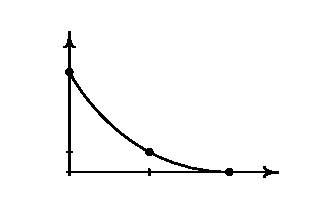
\includegraphics[scale=1.25]{krivka_vyp_t012}\\
   % translate x=-9 y=147 scale 0.30
   \putbox{0.06in}{1.34in}{1.20}{$g(t)$}%
   \putbox{2.11in}{0.09in}{1.20}{$t$}%
   \putbox{1.69in}{0.09in}{1.20}{$t_2$}%
   \putbox{1.02in}{0.09in}{1.20}{$t_1$}%
   \putbox{0.36in}{0.09in}{1.20}{$t_0$}%
   \putbox{0.15in}{0.21in}{1.20}{$G_2$}%
   \putbox{0.15in}{0.38in}{1.20}{$G_1$}%
   \putbox{0.15in}{1.04in}{1.20}{$G_0$}%
   } % close 'parbox'
   } % close 'scalebox'
   \vspace{-\baselineskip} % this is not necessary, but looks better

	\caption{príklad krivky pre vypínací dej}
	\label{fig:krivka_vyp_t012}
\end{figure}


\subsection{Parabola s \uv{nastaviteľným} exponentom}
Hĺbka priehybu parabolickej krivky je daná veľkosťou exponentu. Túto skutočnosť možno využiť k preloženiu analytickej krivky predpokladaného tvaru zmeranými bodmi. Parabola vo všeobecnom tvare $f(t)=a(t+b)^\alpha$ je jednoznačne určená tromi parametrami. Parameter $\alpha$ môže byť párny, nepárny, ako aj neceločíselný (v tom prípade je krivka naznačená na Obr. \ref{fig:patocka_fxfmxfmxpb} vľavo nesymetrická).
\begin{figure}[ht!]
	\centering
	% XCircuit output "skola/5zs/sempr/latex/obr/krivky_patocka_fxfmxfmxpb.tex" for LaTeX input from skola/5zs/sempr/latex/obr/krivky_patocka_fxfmxfmxpb.ps
\def\putbox#1#2#3#4{\makebox[0in][l]{\makebox[#1][l]{}\raisebox{\baselineskip}[0in][0in]{\raisebox{#2}[0in][0in]{\scalebox{#3}{#4}}}}}
\def\rightbox#1{\makebox[0in][r]{#1}}
\def\centbox#1{\makebox[0in]{#1}}
\def\topbox#1{\raisebox{-0.60\baselineskip}[0in][0in]{#1}}
\def\midbox#1{\raisebox{-0.20\baselineskip}[0in][0in]{#1}}
   \scalebox{0.8}{
   \normalsize
   \parbox{5.48438in}{
   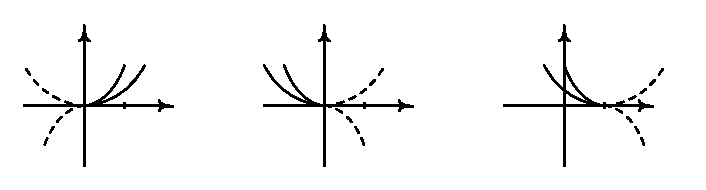
\includegraphics[scale=1.25]{krivky_patocka_fxfmxfmxpb}\\
   % translate x=591 y=207 scale 0.30
   \putbox{0.65in}{1.06in}{1.20}{$f(x)$}%
   \putbox{1.19in}{0.40in}{1.20}{$x$}%
   \putbox{0.86in}{0.40in}{1.20}{$b$}%
   \putbox{2.65in}{1.06in}{1.20}{$f(-x)$}%
   \putbox{3.19in}{0.40in}{1.20}{$x$}%
   \putbox{2.86in}{0.40in}{1.20}{$b$}%
   \putbox{4.65in}{1.06in}{1.20}{$f(-x+b)$}%
   \putbox{5.19in}{0.40in}{1.20}{$x$}%
   \putbox{4.86in}{0.40in}{1.20}{$b$}%
   } % close 'parbox'
   } % close 'scalebox'
   \vspace{-\baselineskip} % this is not necessary, but looks better

	%\caption{K určeniu znamienok vo vzťahu (\ref{eq:})}
	\caption{Operácie so všeobecnou funkciou $f(x)$.}
	\label{fig:patocka_fxfmxfmxpb}
\end{figure}

Úvahou graficky naznačenou na Obr. \ref{fig:patocka_fxfmxfmxpb} možno odvodiť výraz pre vypínací dej:
\begin{equation}
	g_{CE}(t) = 
	\left\{
	\begin{array}{l l}
		G_{CE,sat};	& t<t_0 \\
		G_{CE,sat} \left( 1 - \frac{t-t_0}{t_{off}} \right)^\alpha;	& t_0 \leq t \leq t_0+t_{off} \\
		0;		& t > t_0+t_{off}
	\end{array}
	\right.
	\label{eq:gCE_patocka_valsa}
\end{equation}
kde $t_0$ je okamih počiatku vypínacieho deja, $t_{off}$ je celková vypínacia doba deja, $G_{CE,sat} = \frac{I_L}{U_{CE,sat}}$.
Tento vzťah bol odvodený v \cite{valsa-patocka-petru}. Pre výpočet parametru $\alpha$ autori uvádzajú vzťah:
\begin{equation}
	\alpha = \frac{\ln\left( U_d / U_{CE,sat} \right)}{\ln\left( t_{off} / t_f \right)}
	\label{eq:patocka_alpha}
\end{equation}

Pre zapínací dej autori odvodili obdobný vzťah.

Táto aproximácia sa osvedčila v dobe citovaného článku pre vtedajšie bipolárne tranzistory pre svoju jednoduchosť (pri $t_0 = 0$ a $G_{off} = 0$ stačí zadávať tri čísla z merania) a dobrý súlad so skutočným priebehom $g_{CE} = \frac{i_{C}}{u_{CE}}$. 

Pre súčasné unipolárne a hlavne IGBT tranzistory, kde sa kombinuje rýchle zavretie MOSFET štruktúry s následným pomalším vypínaním štruktúry PNP, s typickým \uv{chvostom} v priebehu $i_C$ môže byť tento jednoduchý model tvarovo nepostačujúci.


\subsection{Interpolačný polynóm}
Väčšiu tvarovú flexibilitu a zároveň jeden funkčný predpis na celom intervale $(t_0, t_2)$ poskytuje interpolácia polynómu zmeranými bodmi.\\
Jednoduchý algoritmus dosadzovania hodnôt priamo z predpisu tabuľkou (\ref{eq:tab_predpis_t012}) poskytuje Lagrangeov polynóm $n$-tého rádu v tvare:
\begin{equation}
	P_n(t) = \sum_{i=0}^n G_i \cdot l_i(t); 
	\;\;\;\;\;\;\;\;\;\;\;\;\;\;\;\;
	l_i(t) = \prod_{j=0,1,\ldots,n; j\neq i} \frac{t - t_j}{t_i - tj}
	\label{eq:Lagrange_vseobec}
\end{equation}
teda napr. pre 3 body z predpisu (\ref{eq:tab_predpis_t012}):
\begin{equation}
	P_2(t) = G_0 \cdot \frac{(t-t_1)(t-t_2)}{(t_0-t_1)(t_0-t_2)} + G_1 \cdot \frac{(t-t_0)(t-t_2)}{(t_1-t_0)(t_1-t_2)} + G_2 \cdot \frac{(t-t_0)(t-t_1)}{(t_2-t_0)(t_2-t_1)}
	\label{Lagrange_z_tabulky}
\end{equation}

\begin{figure}[ht!]
	\centering
	% XCircuit output "Lagrange_vseobec.tex" for LaTeX input from Lagrange_vseobec.ps
\def\putbox#1#2#3#4{\makebox[0in][l]{\makebox[#1][l]{}\raisebox{\baselineskip}[0in][0in]{\raisebox{#2}[0in][0in]{\scalebox{#3}{#4}}}}}
\def\rightbox#1{\makebox[0in][r]{#1}}
\def\centbox#1{\makebox[0in]{#1}}
\def\topbox#1{\raisebox{-0.60\baselineskip}[0in][0in]{#1}}
\def\midbox#1{\raisebox{-0.20\baselineskip}[0in][0in]{#1}}
   \scalebox{0.8}{
   \normalsize
   \parbox{3.02083in}{
   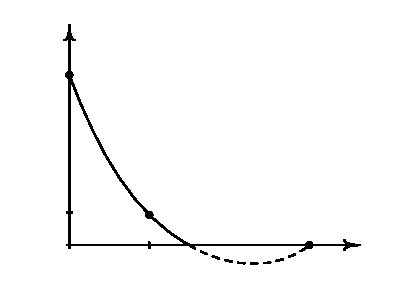
\includegraphics[scale=1.25]{Lagrange_vseobec}\\
   % translate x=-9 y=147 scale 0.30
   \putbox{0.06in}{1.92in}{1.20}{$g(t)$}%
   \putbox{2.77in}{0.09in}{1.20}{$t$}%
   \putbox{2.44in}{0.09in}{1.20}{$t_2$}%
   \putbox{1.02in}{0.09in}{1.20}{$t_1$}%
   \putbox{0.36in}{0.09in}{1.20}{$t_0$}%
   \putbox{0.15in}{0.21in}{1.20}{$G_2$}%
   \putbox{0.15in}{0.48in}{1.20}{$G_1$}%
   \putbox{0.15in}{1.63in}{1.20}{$G_0$}%
   } % close 'parbox'
   } % close 'scalebox'
   \vspace{-\baselineskip} % this is not necessary, but looks better

	\caption{Polynóm 2. stupňa (preložený tromi bodmi).}
	\label{fig:Lagrange_vseobec}
\end{figure}

Primárnym účelom Lagrangeovho polynómu je preloženie krivky danými bodmi; nie je vylúčená situácia znázornená na Obr. \ref{fig:Lagrange_vseobec} (je naopak pomerne pravdepodobná), teda vznik intervalov s kladnou deriváciou (sklonom) či dokonca úsek so zápornou vodivosťou. Takáto situácia je nie len fyzikálne nezmyselná, ale tiež predstavuje výpočtové problémy v prípade zaradenia vodivosti do numericky riešeného obvodu.

Jednoduchý polynóm preložený cez 3 body preto nie je príliš sľubnou aproximáciou.


\subsection{Krivky definované na dvoch subintervaloch s hraničnými podmienkami}

Krivku možno tiež definovať zvlášť na jednotlivých intervaloch medzi danými bodmi:
\begin{equation}
	g_{CE}(t) = 
	\left\{
	\begin{array}{l l}
		G_0;	& t<t_0 \\
		g_1(t);	& t_0 \leq t < t_1 \\
		g_2(t);	& t_1 \leq t < t_2 \\
		G_2;		& t \geq t_2
	\end{array}
	\right.
	\label{eq:krivka_subintervaly_gong1g2goff}
\end{equation}

Požadované vlastnosti výslednej krivky definujú hraničné podmienky pre jednotlivé krivky
.

Pre jednoduchosť definujme na podintervaloch parabolické krivky druhého rádu v názornom tvare pre vynášanie do grafu:

\begin{subequations} 
	\label{eq:def_g1_g2_klm_obe}
	\begin{align}
		g_1(t) = k_1 (l_1 - t)^2 + m_1	%\label{eq:def_g1_g2_klm_1}
		\\
		g_2(t) = k_2 (l_2 - t)^2 + m_2	%\label{eq:def_g1_g2_klm_2}
	\end{align}
\end{subequations}

Roznásobením zátvorky dostaneme po substitúciach
\begin{subequations} 
	\label{eq:subst_klm2abc}
	\begin{align}
		a_i = k_i\\
		b_i = -2 k_i l_i\\
		c_i = k_i l_i^2 + m_i
	\end{align}
\end{subequations}
tvar rovníc zapisovateľný do matice, tj, pre neznáme $a_i$, $b_i$, $c_i$ sa jedná o lineárne rovnice:
\begin{subequations} 
	\label{eq:def_g1_g2_abc_obe}
	\begin{align}
		g_1(t) = a_1 t^2 + b_1 t + c_1	\label{eq:def_g1_g2_abc_1}\\
		g_2(t) = a_2 t^2 + b_2 t + c_2	\label{eq:def_g1_g2_abc_2}
	\end{align}
\end{subequations}

Vo funkciách (\ref{eq:def_g1_g2_abc_obe}) vystupuje 6 neznámych. Na ich vyriešenie je preto nutné zostaviť systém 6 rovníc takých, aby výsledné funkcie spĺňali požadované vlastnosti.\\
Zaveďme teda tieto predpoklady (okrajové podmienky):
\begin{myass}
	$g_1(t_0) = G_0$
	\label{myass:1}
\end{myass}
\begin{myass}
	$g_1(t_1) = G_1$
	\label{myass:2}
\end{myass}
\begin{myass}
	$g_2(t_1) = G_1$
	\label{myass:3}
\end{myass}
\begin{myass}
	$g_2(t_2) = G_2$
	\label{myass:4}
\end{myass}
\begin{myass}
	$g_1'(t_1) = g_2'(t_1)$ \ldots hladkosť krivky v bode $t=t_1$
	\label{myass:5}
\end{myass}
\begin{myass}
	$g_2'(t_2)=0$ \ldots hladkosť v bode $t=t_2$
	\label{myass:6}
\end{myass}
\vspace{12pt}

Derivovaním (\ref{eq:def_g1_g2_klm_obe}) resp. (\ref{eq:def_g1_g2_abc_obe}) podľa času dostávame:

\begin{subequations} 
	\label{eq:def_g1_g2_deriv_klm_obe}
	\begin{align}
		g_1'(t) = -2 k_1 (l_1 -t) 	\label{eq:def_g1_g2_deriv_klm_1} \\
		g_2'(t) = -2 k_2 (l_2 -t) 	\label{eq:def_g1_g2_deriv_klm_2}
	\end{align}
\end{subequations}

\begin{subequations} 
	\label{eq:def_g1_g2_deriv_abc_obe}
	\begin{align}
		g_1'(t) = 2 a_1 t + b_1 	\label{eq:def_g1_g2_deriv_abc_1} \\
		g_2'(t) = 2 a_2 t + b_2 	\label{eq:def_g1_g2_deriv_abc_2}
	\end{align}
\end{subequations}

Dosadením predpokladov (\ref{myass:1}) až (\ref{myass:6}) do (\ref{eq:def_g1_g2_abc_obe}), (\ref{eq:def_g1_g2_deriv_abc_obe}) získame jednoznačne riešiteľnú sústavu v maticovom tvare zapísanú ako:

\begin{equation}
	\underbrace
	{
		\left( 
		\begin{array}{c c c c c c}
			t_0^2& t_0& 1& 0& 0& 0\\
			t_1^2 &t_1 &1 &0 & 0& 0 \\
			0& 0& 0& t_1^2& t_1& 1 \\
			0& 0& 0& t_2^2& t_2& 1 \\
			2t_1& 1& 0& -2t_1& -1& 0 \\
			0& 0& 0& 2t_1& 1& 0
		\end{array}
		\right)
	}_{[M]}
	\cdot
	\underbrace
	{
		\left(
		\begin{array}{c}
			a_1 \\
			b_1 \\
			c_1 \\
			a_2 \\
			b_2 \\
			c_2
		\end{array}
		\right)
	}_{\mathbf{X}}
	=
	\underbrace
	{
		\left( 
		\begin{array}{c}
			G_0 \\
			G_1 \\
			G_1 \\
			G_2 \\
			0 \\
			0
		\end{array}
		\right)
	}_{\mathbf{V}}
	\label{eq:krivka_matica_sustavy}
\end{equation}

kde $[M]$ je matica sústavy, ktorej všetky prvky sú známe (z predpisu (\ref{eq:tab_predpis_t012})), $\mathbf{X}$ je vektor neznámych hľadaných parametrov a $\mathbf{V}$ je známy vektor výsledkov rovníc.

Riešením sústavy je:
\begin{equation}
	\mathbf{X} = [M]^{-1} \cdot \mathbf{V}
	\label{eq:krivka_riesenie_abc}
\end{equation}

V programe \textit{Octave} (alebo \textsc{Matlab}) možno na riešenie takejto sústavy použiť jeden príkaz bez nutnosti vyčísľovania inverznej matice:
\begin{verbatim}
X = M \ V
\end{verbatim}

Program na obvodové simulácie \textsc{Spice} neponúka príliš široké matematické možnosti, čo zvlášť platí pre pôvodnú verziu \textsc{Spice 3} z univerzity v Berkeley, ktorý možno považovať za štandard a preto je jedným z cieľov tejto práce model kompatibilný práve so \textsc{Spice 3}.

Je preto vhodné vyjadriť jednotlivé koeficienty funkcii $g_1$, $g_2$ analyticky. Na tento účel je vhodnejší tvar rovníc (\ref{eq:def_g1_g2_klm_obe}), (\ref{eq:def_g1_g2_deriv_klm_obe}).
Postupným dosadzovaním predpokladov (\ref{myass:6}), (\ref{myass:4}), (\ref{myass:3}) do príslušných rovníc sú vyjadrené koeficienty $l_2$, $m_2$, $k_2$.
Následným dosadením predpokladov (\ref{myass:1}), (\ref{myass:2}), (\ref{myass:5}) sú vyjadrené zvyšné koeficienty $l_1$, $m_1$, $k_1$:

\begin{equation}
	\begin{array}{r l}
		k_2& = \frac{G_1-G_2}{(t_2-t_1)^2} \\
		l_2& = t2 \\
		m_2& = G_2 \\
		l_1& = \frac{(t_1-t_0)^2 (G_1 - G_2) - t_1(t_2-t_1)}{2(t_1-t_0)(G_1-G_2) - (t_2-t_1)(G_0-G_1)} \\
		k_1& = \frac{G_1-G_2}{(t_2-t_1)(l_1-t_1)} \\
		m_1& = G_0 - k1(l_1 - t_0)^2
	\end{array}
	\label{eq:krivka_riesenie_klm}
\end{equation}

Sústavu podobnú sústave (\ref{eq:krivka_matica_sustavy} je jednoduchým spôsobom možné definovať a riešiť numericky pomocou výpočtových programov aj pre zapínací dej a takisto pre viacero subintervalov. V prípade potreby je možné definovať vlastnosti výslednej krivky inými okrajovými podmienkami pre jednotlivé funkcie.

Poznamenajme, že $G_1 = G_{CE,sat}=\frac{I_L}{U_{CE,sat}}$, $G_2 = G_{off} \approx 0$, $t_2 = t_0+t_{off}$ a $t_1$ a $G_1$ závisí na konkrétnej podobe (\ref{eq:tab_predpis_t012}). Koeficienty $a_i$, $b_i$, $c_i$ sú ekvivalentné s koeficientami $k_i$, $l_i$, $m_i$ s prepočítavacím vzťahom cez substitúcie (\ref{eq:subst_klm2abc}).



Metóda dvoch funkcií na subintervaloch je použiteľná aj pre \uv{menej hladké} priebehy, ako je napr. \uv{chvost} vypínaného prúdu IGBT tranzistorom. Na Obr. \ref{fig:tail} je vyobrazený takýto prípad (horšie modelovateľný pomocou jednoduchej paraboly)

\begin{figure}
	\centering
	% GNUPLOT: LaTeX picture with Postscript
\begingroup
  \makeatletter
  \providecommand\color[2][]{%
    \GenericError{(gnuplot) \space\space\space\@spaces}{%
      Package color not loaded in conjunction with
      terminal option `colourtext'%
    }{See the gnuplot documentation for explanation.%
    }{Either use 'blacktext' in gnuplot or load the package
      color.sty in LaTeX.}%
    \renewcommand\color[2][]{}%
  }%
  \providecommand\includegraphics[2][]{%
    \GenericError{(gnuplot) \space\space\space\@spaces}{%
      Package graphicx or graphics not loaded%
    }{See the gnuplot documentation for explanation.%
    }{The gnuplot epslatex terminal needs graphicx.sty or graphics.sty.}%
    \renewcommand\includegraphics[2][]{}%
  }%
  \providecommand\rotatebox[2]{#2}%
  \@ifundefined{ifGPcolor}{%
    \newif\ifGPcolor
    \GPcolorfalse
  }{}%
  \@ifundefined{ifGPblacktext}{%
    \newif\ifGPblacktext
    \GPblacktexttrue
  }{}%
  % define a \g@addto@macro without @ in the name:
  \let\gplgaddtomacro\g@addto@macro
  % define empty templates for all commands taking text:
  \gdef\gplbacktext{}%
  \gdef\gplfronttext{}%
  \makeatother
  \ifGPblacktext
    % no textcolor at all
    \def\colorrgb#1{}%
    \def\colorgray#1{}%
  \else
    % gray or color?
    \ifGPcolor
      \def\colorrgb#1{\color[rgb]{#1}}%
      \def\colorgray#1{\color[gray]{#1}}%
      \expandafter\def\csname LTw\endcsname{\color{white}}%
      \expandafter\def\csname LTb\endcsname{\color{black}}%
      \expandafter\def\csname LTa\endcsname{\color{black}}%
      \expandafter\def\csname LT0\endcsname{\color[rgb]{1,0,0}}%
      \expandafter\def\csname LT1\endcsname{\color[rgb]{0,1,0}}%
      \expandafter\def\csname LT2\endcsname{\color[rgb]{0,0,1}}%
      \expandafter\def\csname LT3\endcsname{\color[rgb]{1,0,1}}%
      \expandafter\def\csname LT4\endcsname{\color[rgb]{0,1,1}}%
      \expandafter\def\csname LT5\endcsname{\color[rgb]{1,1,0}}%
      \expandafter\def\csname LT6\endcsname{\color[rgb]{0,0,0}}%
      \expandafter\def\csname LT7\endcsname{\color[rgb]{1,0.3,0}}%
      \expandafter\def\csname LT8\endcsname{\color[rgb]{0.5,0.5,0.5}}%
    \else
      % gray
      \def\colorrgb#1{\color{black}}%
      \def\colorgray#1{\color[gray]{#1}}%
      \expandafter\def\csname LTw\endcsname{\color{white}}%
      \expandafter\def\csname LTb\endcsname{\color{black}}%
      \expandafter\def\csname LTa\endcsname{\color{black}}%
      \expandafter\def\csname LT0\endcsname{\color{black}}%
      \expandafter\def\csname LT1\endcsname{\color{black}}%
      \expandafter\def\csname LT2\endcsname{\color{black}}%
      \expandafter\def\csname LT3\endcsname{\color{black}}%
      \expandafter\def\csname LT4\endcsname{\color{black}}%
      \expandafter\def\csname LT5\endcsname{\color{black}}%
      \expandafter\def\csname LT6\endcsname{\color{black}}%
      \expandafter\def\csname LT7\endcsname{\color{black}}%
      \expandafter\def\csname LT8\endcsname{\color{black}}%
    \fi
  \fi
  \setlength{\unitlength}{0.0500bp}%
  \begin{picture}(4320.00,4320.00)%
    \gplgaddtomacro\gplbacktext{%
      \csname LTb\endcsname%
      \put(176,2379){\rotatebox{-270}{\makebox(0,0){\strut{}$g_{CE}$, $v_{CE}$, $i_C$}}}%
      \put(2159,440){\makebox(0,0){\strut{}ČAS}}%
    }%
    \gplgaddtomacro\gplfronttext{%
    }%
    \gplgaddtomacro\gplbacktext{%
      \csname LTb\endcsname%
      \put(396,2379){\rotatebox{-270}{\makebox(0,0){\strut{}}}}%
      \put(2159,594){\makebox(0,0){\strut{}}}%
    }%
    \gplgaddtomacro\gplfronttext{%
    }%
    \gplgaddtomacro\gplbacktext{%
      \csname LTb\endcsname%
      \put(396,2379){\rotatebox{-270}{\makebox(0,0){\strut{}}}}%
      \put(2159,594){\makebox(0,0){\strut{}}}%
    }%
    \gplgaddtomacro\gplfronttext{%
    }%
    \gplbacktext
    \put(0,0){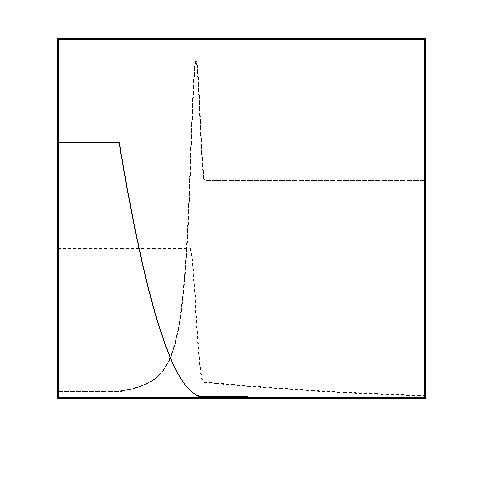
\includegraphics{./tail}}%
    \gplfronttext
  \end{picture}%
\endgroup

	\caption{Možnosti modelu definovaného dvomi krivkami na podintervaloch.}
	\label{fig:tail}
\end{figure}



\chapter{Výsledky meraní a simulácie} \label{ch:vysledky}

\section{Použité súčiastky a prístroje}

Priebehy spínacích dejov boli zmerané na nasledovných spínacích súčiastkach:
\begin{itemize}
    \item BJT: BUX48A
    \item IGBT: G50N60HS
\end{itemize}
V oboch prípadoch bola použitá nulová dioda typu
\begin{itemize}
    \item IDP45E60
\end{itemize}

V usporiadaní podľa Obr. \ref{fig:schema_pracovisko} bol na merania použitý batériovo napájaný 4-kanálový $500\un{MHz}$ osciloskop \textit{Agilent DSO6054A} (sériové číslo MY48200002).

Bočník bol pre potlačenie vplyvu jeho parazitnej indukčnosti volený o veľkej hodnote $R_b = 1\un{\Omega}$, a takisto pre zníženie indukčnosti je konštruovaný tesným paralelným spojením 10 kusov SMD rezistorov.

Bipolárny tranzistor bol budený v zapojení s indukčnosťou $8\un{\mu H}$ v sérii s prechodom báza-emitor. Jedná sa o odporučené zapojenie z hľadiska obmedzenia rozširovacieho javu.

Tranzistor IGBT bol budený cez odpor $R_G = 5 \un{\Omega}$, čo je výrobcom odporučená katalógová hodnota. Odpor $R_G$ bol zapojený medzi emitorom (tj. meracou zemou) a zápornou budiacou svorkou, čím sa z neho stáva zároveň bočník snímajúci nabíjací prúd $i_G$.


\newpage
\section{Simulátor a model $g_{CE}$} \label{sec:simulator}

V SPICE 3 (i skorších verziách) je možné definovať premenlivý odpor (\textit{behavioral resistor}), ako aj zdroje, syntaxou:
\begin{verbatim}
RXXXX n+ n- r = 'expression'
\end{verbatim}
kde \texttt{'expression'} je výraz závislý na konštantách alebo napätiach v obvodových uzloch (v novších verziách SPICE je možné použiť programom definované premenné ako čas, teplota a podobne; v prípade že simulátor takúto možnosť neposkytuje, je možné vytvoriť jednotkový kondenzátor nabíjaný jednotkovým prúdom - potom napätie na ňom zodpovedá času).

V tejto práci je premenná vodivosť modelovaná podobným spôsobom - v prostredí \textit{Octave} sa vypočítajú parametre vodivosti a zapíše sa na disk súbor obsahujúci SPICE model časovo závislého zdroja napätia s napätím rovným $g_{CE}(t)$:
\begin{verbatim}
Bgce ngce 0 v = 'expression'
\end{verbatim}
kde \texttt{expression} je výraz (\ref{eq:krivka_subintervaly_gong1g2goff}) zapísaný pomocou SPICE syntaxe ternary operátora. Tento súbor je zahrnutý do simulačného netlistu pomocou príkazu \texttt{.include} a vodivosť je modelovaná premenlivým odporom:
\begin{verbatim}
Rce ne nc r = '1/v(ngce)'
\end{verbatim}

Príklad simulačného netlistu a zodpovedajúca obvodová schéma sú priložené v Dodatku \ref{ch:priloha_sim}.

\newpage
\section{Zmerané priebehy BJT} \label{sec:vysl_BJT}

\subsection{Vypínací dej}

\myfigtex{obr/plots/bjt_300_10_off}{Vypínací dej BJT - $300\un{V}$, $10\un{A}$}{\label{fig:plot_bjt_300_10_off}}
\myfigtex{obr/plots/sim_par_bezpar_bjt_300_10_off}{Detail simulácie vypínacieho deja BJT bez parazitných prvkov a s parazitnými prvkami.}{\label{fig:plot_bjt_300_10_off_detail}}
\myfigtex{obr/schema_sim_par_R1C1L3}{Príklad zahrnutia pozorovaných parazitných vplyvov}{\label{fig:schema_sim_par_R1C1L3}}

\myfigtex{obr/plots/bjt_300_08_off}{Vypínací dej BJT - $300\un{V}$, $8\un{A}$}{\label{fig:plot_bjt_300_10_off}}

\myfigtex{obr/plots/bjt_300_06_off}{Vypínací dej BJT - $300\un{V}$, $6\un{A}$}{\label{fig:plot_bjt_300_10_off}}

\myfigtex{obr/plots/bjt_300_04_off}{Vypínací dej BJT - $300\un{V}$, $4\un{A}$}{\label{fig:plot_bjt_300_10_off}}

\FloatBarrier


\subsection{Zapínací dej}

Na Obr. \ref{fig:plot_bjt_300_10_on} sú uvedené zmerané priebehy zapínacieho deja. Rekonštruovaná vodivosť $g_{CE}(t)$ nespĺňa predpoklad hladkého priebehu. V počiatočnej fáze deja, v dobe prudkého nárastu prúdu je vodivosť evidentne znížená oproti hladkému pokračovaniu priebehu vo zvyšných fázach deja. Prvé vysvetlenie by viedlo k Obr. \ref{fig:sim_L2} v kapitole \ref{ch:parazity}. Indukčnosť spojov elektród deformuje merateľný priebeh zapínacieho deja práve spôsobom, kedy je v dobe veľkých hodnôt $\dxdt{i}{t}$ merané väčšie napätie, než je skutočné napätie na čipe (kde je v skutočnosti prítomný podkmit), čo sa prejaví na zmenšenej hodnote podielu meraných hodnôt $\frac{i_C}{u_{CE}}$. Je však jednoducho vyčísliteľné, že aby došlo k tak výraznému poklesu vodivosti (nemerateľnému podkmitu napätia), musela by byť indukčnosť prívodov v rádoch $\mu H$, čo s určitosťou nie je.

Vysvetlením je skôr iný účinok tejto indukčnosti (a indukovaného napätia na nej). Keďže riadiaca zem budiča je k tranzistoru pripojená v na silový emitorový vývod, napätie indukované zmenou silového prúdu na úseku medzi bodom pripojenia a emitorom čipu má za následok stav, kedy je skutočné emitorové napätie na vyššej úrovni, ako riadiaca zem (tá ostane neovplyvnená, kým potenciál emitoru je zvýšený). Keďže budiaci obvod ostáva bez zmeny, medzi emitorom čipu a bázou je zmenšené napätie. To ale priviera tranzistor - čo sa prejaví jeho zmenšenou vodivosťou a následne tiež spomalením deja.

\myfigtex{obr/plots/bjt_300_10_on}{Zapínací dej BJT - $300\un{V}$, $10\un{A}$}{\label{fig:plot_bjt_300_10_on}}

\myfigtex{obr/plots/sim_par_bezpar_bjt_300_10_on}{Detail simulácie zapínacieho deja BJT bez parazitných prvkov a s parazitnými prvkami.}{\label{fig:plot_bjt_300_10_on_detail}}

\myfigtex{obr/plots/bjt_zap_ube}{Priebehy zapínacieho deja vrátane bázového napätia s indukčným prekmitom v dobe veľkých hodnôt $\dxdt{i}{t}$.}{\label{fig:bjt_zap_ube}}


%\myfigtex{obr/plots/bjt_300_08_on}{Zapínací dej BJT - $300\un{V}$, $8\un{A}$}{\label{fig:plot_bjt_300_10_on}}

%\myfigtex{obr/plots/bjt_300_06_on}{Zapínací dej BJT - $300\un{V}$, $6\un{A}$}{\label{fig:plot_bjt_300_10_on}}

%\myfigtex{obr/plots/bjt_300_04_on}{Zapínací dej BJT - $300\un{V}$, $4\un{A}$}{\label{fig:plot_bjt_300_10_on}}

\subsection{(Ne)závislosť časového priebehu $g_{CE}(t)$ na napätí medziobvodu}
\myfigtex{obr/plots/bjt_porov_300V_150V_off}{Priebehy vypínania pri rôznych hodnotách $U_d$. }{\label{fig:bjt_porov_300V_150V}}
Merania na bipolárnom tranzistore (Obr. \ref{fig:bjt_porov_300V_150V} potvrdili, že časový priebeh $g_{CE}(t)$ a teda ani celková vypínacia doba sa s napätím nemení. Rozdielné doby $t_d$ a $t_f$ sú dané okamihom prepólovania nulovej diody.


\subsection{Závislosť spínacích časov na prúde}

Priebeh vodivosti a teda aj spínacích časov je závislý na vypínanom prúde (ako plynie aj zo stručnej analýzy v kapitole \ref{ch:gce}). Zmeraná závislosť vypínacieho času na veľkosti prúdu je vynesená graficky na Obr. \ref{fig:bjt_tfi}.

\myfigtex{obr/plots/bjt_tfi}{Závislosť vypínacej doby na vypínanom prúde}{\label{fig:bjt_tfi}}


\newpage
\section{Zmerané piebehy IGBT} \label{sec:vysl_IGBT}

Zmerané boli aj základné spínacie priebehy na tranzistore IGBT. 

Zapínací (a v menej očividnej miere aj vypínací) dej je znovu ovplyvnený indukovaným napätím na parazitnej indukčnosti medzi riadiacim emitorom a emitorom čipu. 


\myfigtex{obr/plots/igbt_300_40_1_off}{Vypínací dej IGBT - $300\un{V}$, $40\un{A}$, $R_G = 5 \un{\Omega}$.}{\label{fig:plot_igbt_300_40_1_off}}

\myfigtex{obr/plots/igbt_300_40_1_on}{Zapínací dej IGBT - $300\un{V}$, $40\un{A}$, $R_G = 5 \un{\Omega}$.}{\label{fig:plot_igbt_300_40_1_on}}

Konkrétny tvar krivky $g_{CE}(t)$ na obrázkoch v počiatku vypínacieho resp. na konci zapínacieho deja nie celkom presne zodpovedá podielu $frac{i_C}{u_{CE}}$, avšak v týchto oblastiach je vplyv  konkrétneho tvaru krivky na výsledné priebehy malý. Plne tak postačuje aproximácia odvodená v kapitole \ref{ch:krivka}, i keď sú samozrejme možné aj iné, snáď výstižnejšie aproximácie.

Podstatnou je však výstižnosť modelu. Jednou z možností jej overenia je aj zaradenie parazitných prvkov resp. odporu bočníka (ktorý popísaným spôsobom úbytkom skresľuje priebeh kolektorového napätia) do obvodu. Po zaradení odporu $1\un{\Omega}$, indukčnosti cca. $50\un{nH}$ (ako sa dá približne spočítať aj z veľkosti vypínacieho prekmitu) a kapacity cca $100\un{pF}$ do obvodu na Obr. \ref{fig:schema_sim_par_R1C1L3} dostaneme priebehy na Obr. \ref{fig:plot_igbt_300_40_1_off_par} a Obr. \ref{fig:plot_igbt_300_40_1_on_par}. Tie sú v dobrom súlade s meranými priebehmi (\uv{prekmit} prúdu pri zapínaní simulovaný nie je, pretože je použitá dioda s ideálnou charakteristikou).

\myfigtex{obr/plots/igbt_300_40_1_off_par}{Vypínací dej IGBT - $300\un{V}$, $40\un{A}$, $R_G = 5 \un{\Omega}$.}{\label{fig:plot_igbt_300_40_1_off_par}}

\myfigtex{obr/plots/igbt_300_40_1_on_par}{Zapínací dej IGBT - $300\un{V}$, $40\un{A}$, $R_G = 5 \un{\Omega}$.}{\label{fig:plot_igbt_300_40_1_on_par}}




%\input{./kapitoly/realiz}

\chapter*{Záver} \label{ch_zaver} \addcontentsline{toc}{chapter}{Záver}
\markboth{\MakeUppercase{Záver}}{\MakeUppercase{Záver}} % aby to aj v hlavicke strany pisalo zaver a nie nieco predchádzajuce, napr. zoznam obrazkov


\lettrine{V}{ rámci} práce sa podarilo vytvoriť meracie pracovisko na presné oscilografické zaznamenanie spínacích dejov; otestované bolo na meraniach bipolárnych a IGBT tranzistorov. Analýza nameraných priebehov naznačuje, že prítomné parazitné vplyvy nie sú významným spôsobom zapríčinené nesprávnym spôsobom snímania.

Ako snímač prúdu je po viacerých pokusoch (s prúdovým transformátorom, Rogowského cievkou aj drahými komerčnými snímačmi) osvedčený SMD bočník s pomerne veľkou hodnotou odporu ($1\un{\Omega}$). Problémy so šírkou snímaného pásma pri proporcionálnej súčiastke akou je odpor nie sú a derivačný charakter spôsobený parazitnou indukčnosťou je potlačený práve veľkou hodnotou odporu. Príliš veľkú hodnotu však voliť nemožno, a to nie len kvôli úbytku napätia, ale aj pre tlmenie, ktorým by mohol skresľovať kmitavé javy v meranom obvode.

Z meraní vyplynula potreba oddeleného silového emitorového kontaktu od riadiaceho. Dôvodom je indukčnosť prívodu a ňou indukované napätie pri veľkých zmenách prúdu (tj. pri spínaní), ktoré spôsobuje rozdiel medzi potenciálom riadiacej (meracej) zeme a skutočným potenciálom emitora na čipe. Dôsledkom toho je nie len skreslený meraný údaj, ale hlavne možné spomalenie spínacieho deja, ako bolo popísané v kapitole \ref{ch:vysledky}. Tento jav býva pozorovaný najmä pri veľkých mnohočipových výkonových moduloch \cite{khanna}. Pozorovaný bol však v tejto práci aj u diskrétnych jednočipových súčiastkach. Manipuláciou s geometrickým usporiadaním resp. dĺžkou prívodov bolo možné ovplyvňovať spínacie deje z pohľadu času rádovo aj o $30\%$. Aj pri úplnom skrátení vývodov z púzdra sú ale elektródy čipu kontaktované s vývodmi pomocou bondovacích drátov, ktorých indukčnosť (ako sa ukázalo) rozhodne nemožno zanedbať. To ilustruje nevhodnosť klasických trojvývodových súčiastok pre rýchle aplikácie.

Parazitné javy (ako bolo ilustrované v kapitole \ref{ch:parazity}) majú za následok väčšie či menšie skreslenie skutočného prúdu a napätia na čipe. To však znamená, že nie všetká energia $\int u_{CE}(t) i_C(t) \dif t$ počas jedného prechodného deja je skutočnou stratovou energiou. Vo všeobecnosti ale možno usúdiť, že množstvo energie, ktoré by sa akumulovalo v parazitnom prvku počas jedného z dejov (čím by sa stalo meranie pesimistickým), sa zase uvoľní a zmarí na teplo počas druhého z dejov, čím súčiastke naopak \uv{prihorší}. Výslednú stratovú bilanciu teda možno považovať viac-menej za neskreslenú aj na pri nedokonalých meraniach.
Navyše, správnym návrhom aplikácie alebo merania je možné najpodstatnejšie parazitné vplyvy odstrániť.

V neposledom rade je súčasťou práce vytvorený \uv{dvojpólový} simulačný model aproximujúci časovú zmenu vodivosti tranzistora $g_{CE}$. Svojou jednoduchosťou oprosťuje simulácie od potrebného veľkého výpočtového výkonu (a dlhých časov simulácií), ako aj od problémov s konvergenciou výpočtov. Zostavenie modelu je veľmi priamočiare; vychádza priamo zo zmeraných priebehov.

Idealizované priebehy produkované takýmto modelom je veľmi jednoducho možné korigovať pridaním parazitných prvkov. Na obrázkoch v stati \ref{sec:vysl_IGBT} zreteľne vidno, že pridané obvodové prvky korigujú idealizované priebehy presne podľa očakávania.

% zhodnotit, ze sa da simulovat, a ze pridanie parazit (kond.) koriguje priebehy podla ocakavania


\begin{thebibliography}{99}

	\bibitem{gummel-poon}{\textsc{Gummel, H. K.}: ``A Charge Control Relation for Bipolar Transistors'', \textit{Bell Syst. Tech. J.}, vol. 49, 1970}
	
	\bibitem{pierret}{\textsc{Pierret, R. F.}: \textit{Semiconductor Device Fundamentals}, Addison-Wesley Publishing Comany, 1996, ISBN 0-201-54393-1}
	
	\bibitem{baliga}{\textsc{Baliga, B. J.}: \textit{Fundamentals of Power Semiconductor Devices}, Springer, 2008, ISBN 978-0-387-47313-0}
	
	\bibitem{hefner}{\textsc{Hefner, A. R., Diebolt, D. M.}: ``An experimentally Verified IGBT Model Implemented in the Saber Circuit Simulator''}, \textit{IEEE Trans. Pwr.Elec., Vol.9, No.5, pp.532-542, Sept. 1994.}
	
	\bibitem{valsa-patocka-petru}{\textsc{Valsa, J., Patočka, M., Petrů, F}: \uv{Jednoduchý matematický model výkonového spínacího tranzistoru}, \textit{Elektrotechnický obzor}, č. 5, 1988.}
	
	\bibitem{patocka:kniha}{\textsc{Patočka, M.}: \textit{Magnetické jevy a obvody ve výkonové elektronice, měřicí technice a silnoproudé elektrotechnice.} Brno: VUTIUM, 2011. 564 s. ISBN 978-80-214-4003-6.}

	\bibitem{shockley}{\textsc{Shockley, W.}: \textit{Electrons and Holes in Semiconductors}, D. van Nostrand Co., 1959, $7^{\mathrm{th}}$ printing}

	\bibitem{lutz}{\textsc{Lutz, J., Schlangenotto, H., Scheuermann, U., De Dockner, R.,}: \textit{Semiconductor Power Devices: Physics, Characteristics, Reliability} Springer, 2011, ISBN 978-3-642-11125-9}

	\bibitem{khanna}{\textsc{Khanna, V. K.,}: \textit{IGBT: Theory and Design}, A Wiley-Interscience publication, 2003, ISBN 0-417-23845-7}

	\bibitem{kondenzator-polypropylen}{MKP1848 Metalized Polypropylene Film Capacitors, DC-Link Capacitor, Datasheet. [cit.2016-1-4] dostupné z \url{www.vishay.com/docs/28164/mkp1848dcl.pdf}}
	
	\bibitem{kondenzator-elektrolyt}{B43508 Aluminum electrolytic capacitors, Datasheet. [cit.2016-1-4] dostupné z \url{http://en.tdk.eu/inf/20/30/db/aec_2015/B43508.pdf}}
	
	\bibitem{tirpak}{\textsc{Tirpák, A.}: \textit{Elektromagnetizmus} (1. vyd.). Bratislava: Univerzita Komenského, FMFI, 1999. 711 s. ISBN 80-88780-26-8.}

	\bibitem{patocka-skripta-3}{\textsc{Patočka, M.}: \textit{Vybrané statě z výkonové elektroniky: Svazek III, Výkonové polovodičové spínací součástky.}[Skriptum.] Brno: VUT, FEKT, 2014, 178s.}


\end{thebibliography}






%\input{./kapitoly/prilohy}
\appendix

\chapter{Obvodové schémy, zoznam súčiastok a DPS} \label{ch:priloha_schemy}

\newpage
\section{Budič výkonových tranzistorov} \label{sec:append_budic}

\hspace{-1.8cm}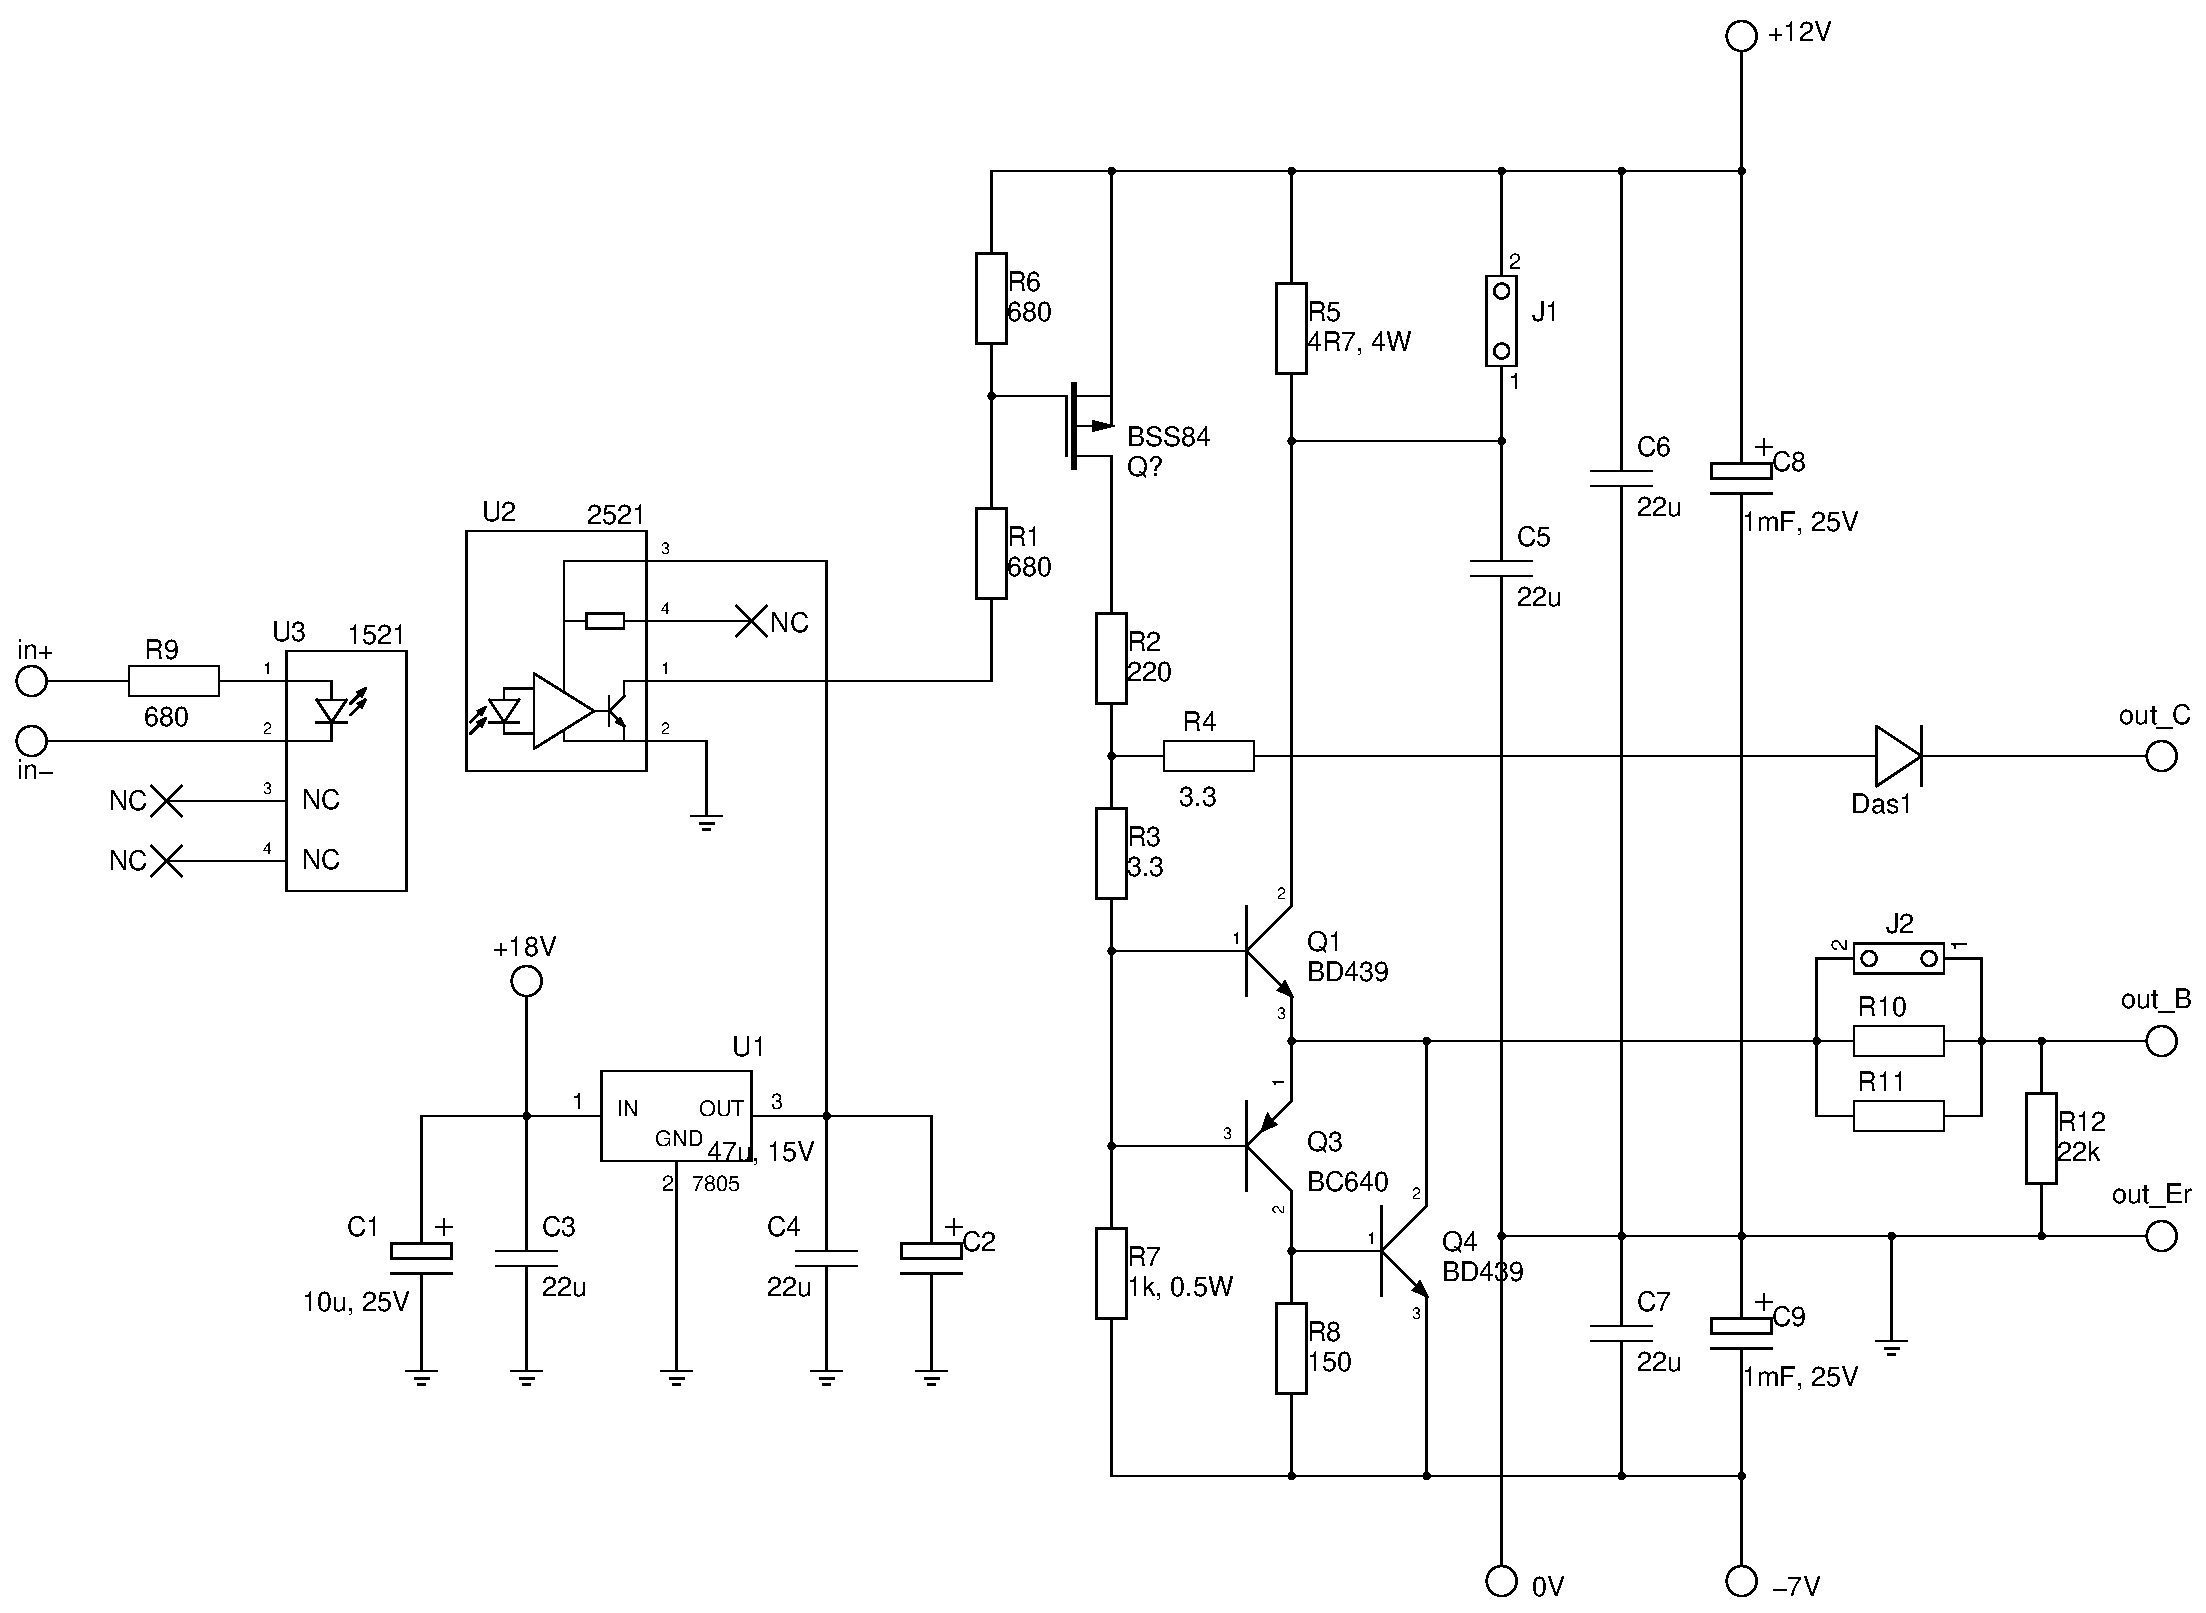
\includegraphics[width=1.2\textwidth]{schema_budic2}


\subsection{DPS}
DPS a rozmiestnenie súčiastok(1:1). Zľava: top assembly, bottom, bottom assembly:\vspace{0pt}

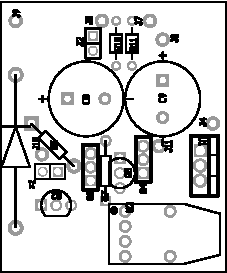
\includegraphics{pcb_budic_top_ass}
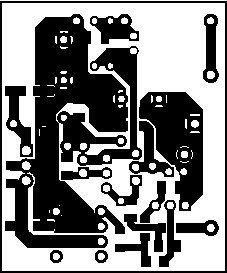
\includegraphics{pcb_budic_bot}
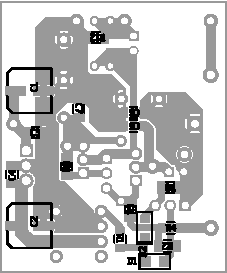
\includegraphics{pcb_budic_bot_ass}

\newpage
\subsection{Zoznam súčiastok}
\small
\begin{verbatim}

refdes   device                    footprint                     value    

C1       POLARIZED_CAPACITOR       NICHICON_WT_CAP_6p3_7p7       10u/25V
C2       POLARIZED_CAPACITOR       NICHICON_WT_CAP_6p3_7p7       47u/15V
C3       CAPACITOR                 1206.fp                       22u
C4       CAPACITOR                 1206.fp                       22u
C5       CAPACITOR                 1206.fp                       22u
C6       CAPACITOR                 1206.fp                       22u
C7       CAPACITOR                 1206.fp                       22u
C8       POLARIZED_CAPACITOR       RCY250P                       1mF/25V
C9       POLARIZED_CAPACITOR       RCY250P                       1mF/25V
D1       DIODE                     minimelf                      1N4148
D2       DIODE                     minimelf                      1N4148
Das1     DIODE                     DIODE_LAY 800.fp              [1000V]
J1       JUMPER                    JUMPER2.fp                             
J2       JUMPER                    JUMPER2.fp                             
Q1       NPN_TRANSISTOR            TO126W.fp                     BD439    
Q2       PNP_TRANSISTOR            TO92.fp                       BC640    
Q3       PNP_TRANSISTOR            TO92.fp                       BC640    
Q4       NPN_TRANSISTOR            TO126W.fp                     BD439    
R1       RESISTOR                  1206.fp                       3k3      
R2       RESISTOR                  1206.fp                       220      
R3       RESISTOR                  1206.fp                       33       
R4       RESISTOR                  1206.fp                       33       
R5       RESISTOR                  ACY400                        "4R7/4W"          
R6       RESISTOR                  1206.fp                       1k       
R7       RESISTOR                  ACY300                        "2k2/0.5W"        
R8       RESISTOR                  1206.fp                       150
R9       RESISTOR                                                680
R10      RESISTOR                  0.125W_Carbon_Resistor                 
R11      RESISTOR                  0.125W_Carbon_Resistor                 
R12      RESISTOR                  1206.fp                       22k      
U1       7805                      TO220W.fp                              
U2       fiber_optic_receiver                                    2521     
U3       fiber_optic_transmitter                                 1521     
\end{verbatim}
\normalsize
\newpage
\section{Napájací obvod budiča} \label{sec:append_nap}
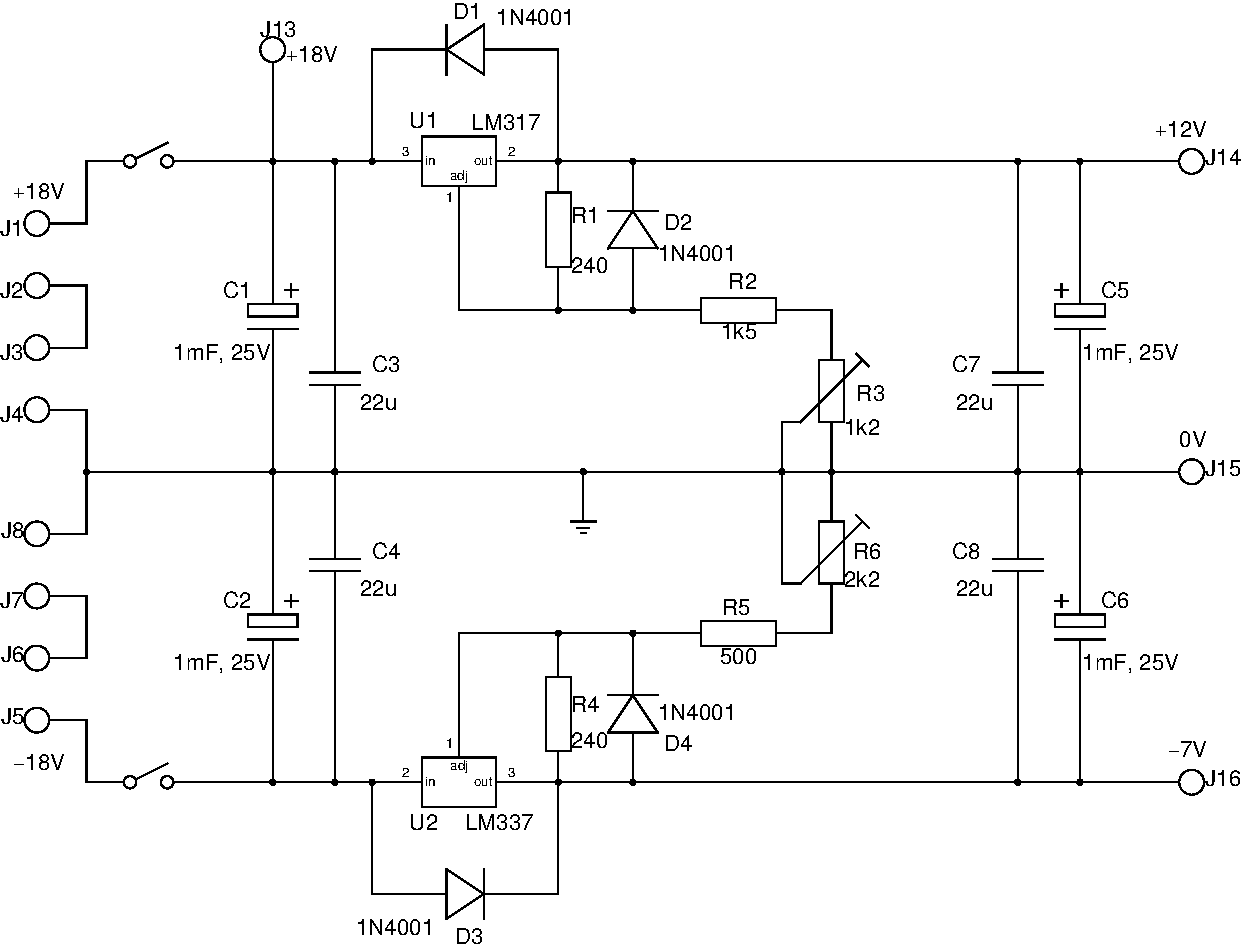
\includegraphics[width=.8\textwidth]{schema_nap}

\subsection{DPS}
DPS a rozmiestnenie súčiastok. Zľava: top assembly, bottom, bottom assembly:\vspace{5pt}

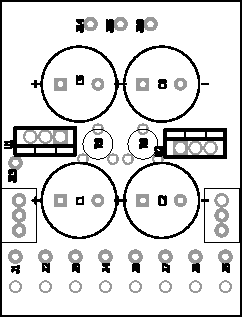
\includegraphics{pcb_nap_top_ass}
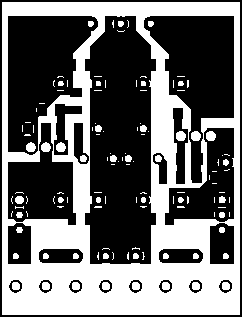
\includegraphics{pcb_nap_bot}
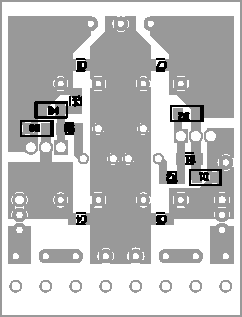
\includegraphics{pcb_nap_bot_ass}

\newpage
\subsection{Zoznam súčiastok}
\small
\hspace{2cm}
\begin{verbatim}
refdes   device                         footprint            value    

C1       POLARIZED_CAPACITOR            RCY250P              1mF/25V
C2       POLARIZED_CAPACITOR            RCY250P              1mF/25V
C3       CAPACITOR                      1206                 22u      
C4       CAPACITOR                      1206                 22u      
C5       POLARIZED_CAPACITOR            RCY250P              1mF/25V
C6       POLARIZED_CAPACITOR            RCY250P              1mF/25V
C7       CAPACITOR                      1206                 22u      
C8       CAPACITOR                      1206                 22u      
D1       DIODE                          melf                 1N4007   
D2       DIODE                          melf                 1N4007   
D3       DIODE                          melf                 1N4007   
D4       DIODE                          melf                 1N4007   
R1       RESISTOR                       1206                 240      
R2       RESISTOR                       1206                 1k5      
R3       VARIABLE_RESISTOR              trimmer_lezaty_5mm   1k2      
R4       RESISTOR                       1206                 240      
R5       RESISTOR                       1206                 500      
R6       VARIABLE_RESISTOR              trimmer_lezaty_5mm   2k2      
U1       adjustable_voltage_regulator   TO220W               LM317    
U2       adjustable_voltage_regulator   TO220W               LM337    
\end{verbatim}
\normalsize




\newpage
\section{Generátor impulzov} \label{sec:append_gen}

\subsection{Schéma zapojenia}
\hspace{-1.0cm}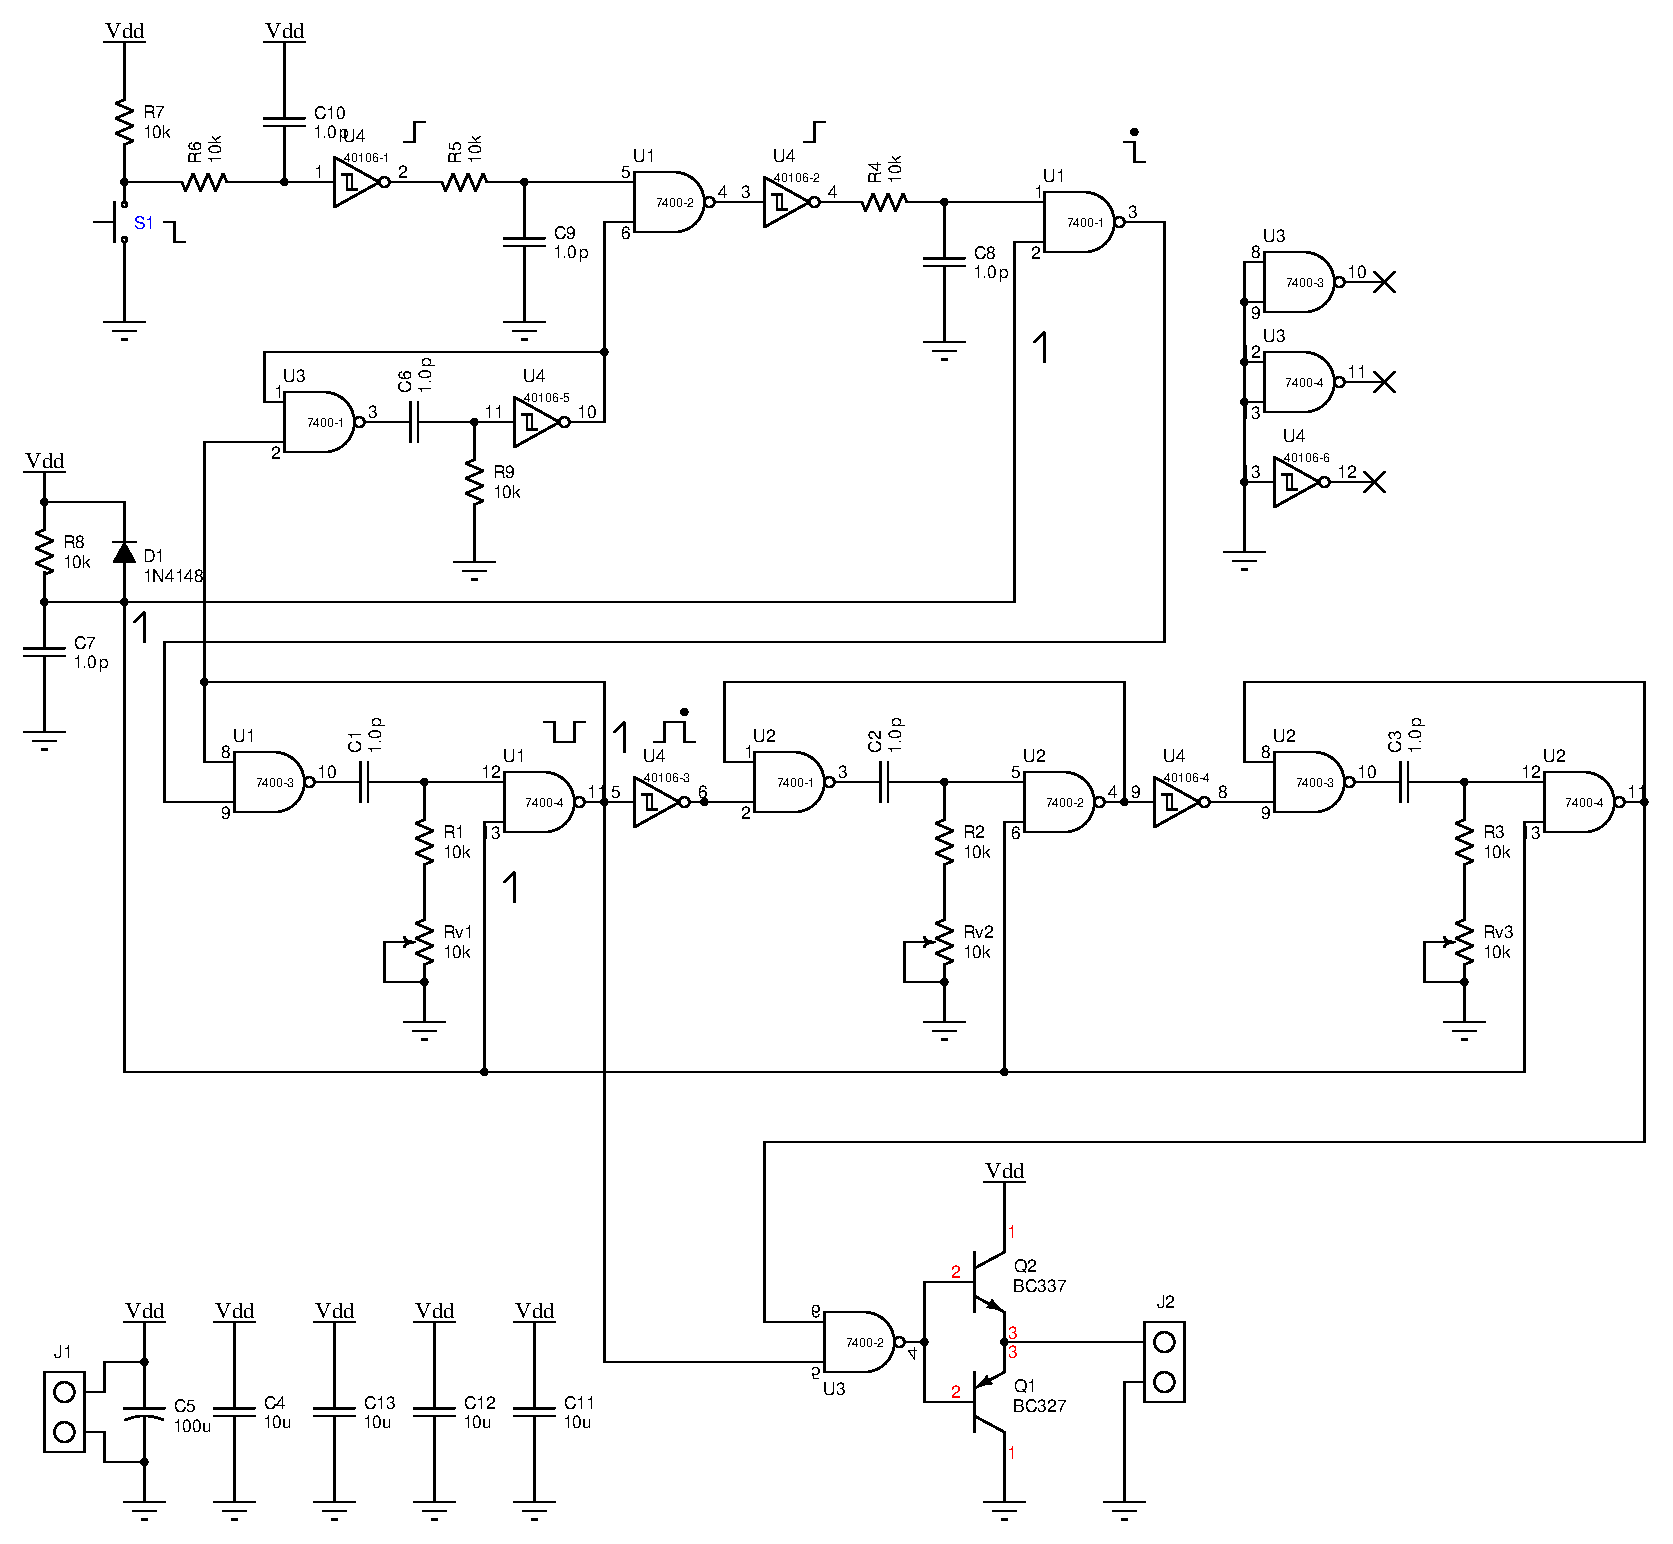
\includegraphics[width=1.25\textwidth]{schema_gen}

\newpage
\subsection{DPS}
DPS a rozmiestnenie súčiastok (1:1). Zľava: top assembly, bottom:\vspace{5pt}

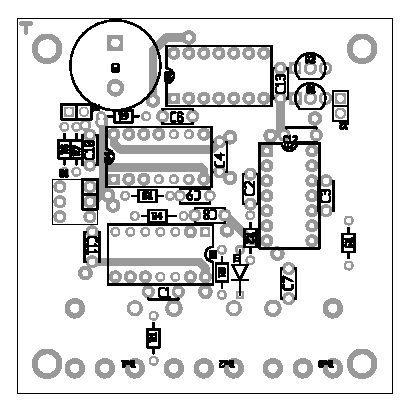
\includegraphics{pcb_gen_top_ass}

\includegraphics{pcb_gen_bot}

%\newpage
%\subsection{Zoznam súčiastok}
%\small
%\hspace{2cm}
%\begin{verbatim}
%\end{verbatim}
\normalsize



\newpage
\section{Medziobvod} \label{sec:append_medziobvod}

\subsection{Schéma zapojenia}
\vspace{10pt}
\hspace{-1.0cm}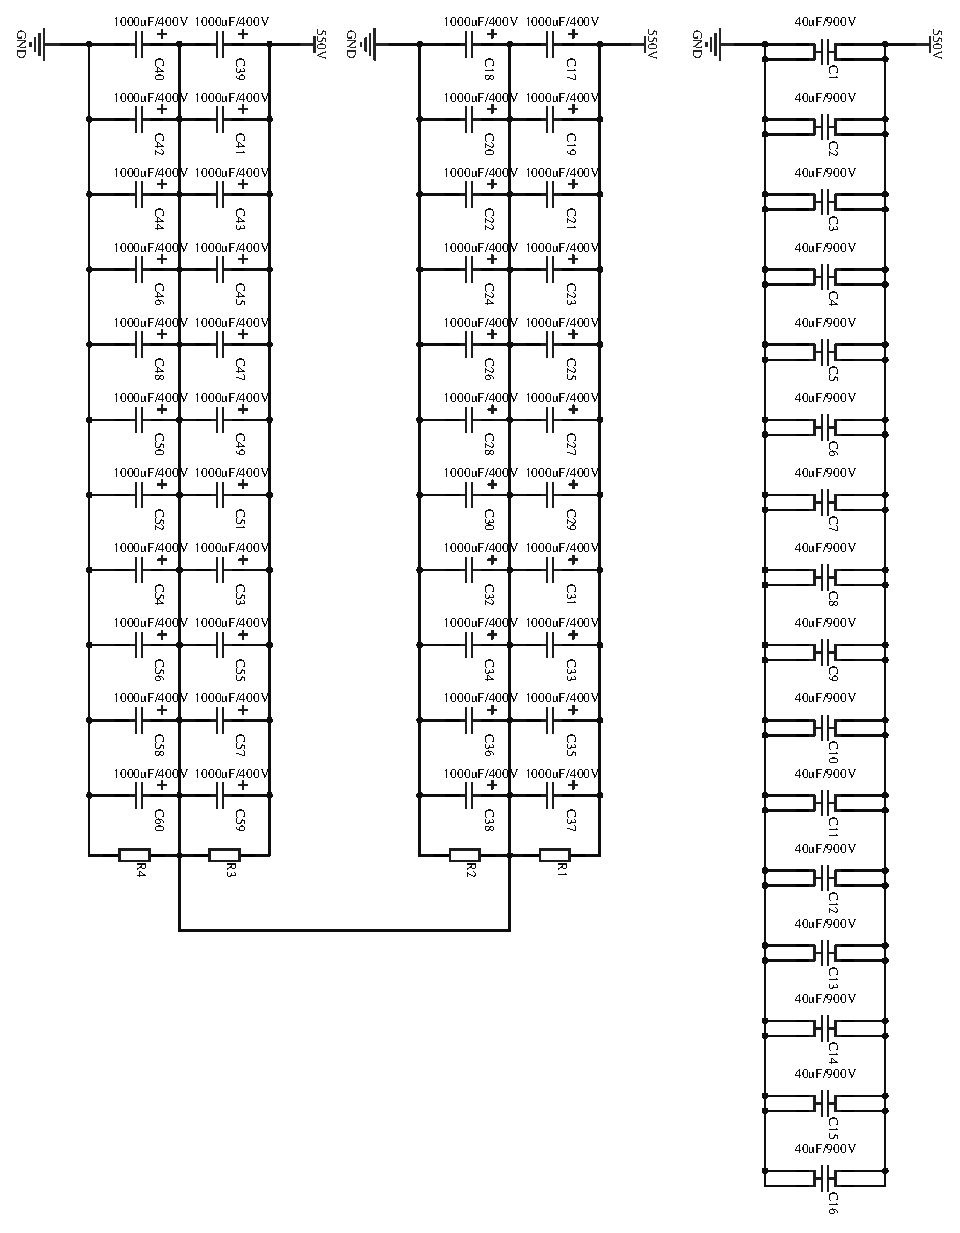
\includegraphics[width=1.1\textwidth]{schema_medziobvod_90}

\newpage
\subsection{DPS}
DPS a rozmiestnenie súčiastok (zmenšené). V poradí: top, bottom, bottom assembly:\vspace{5pt}
\centering
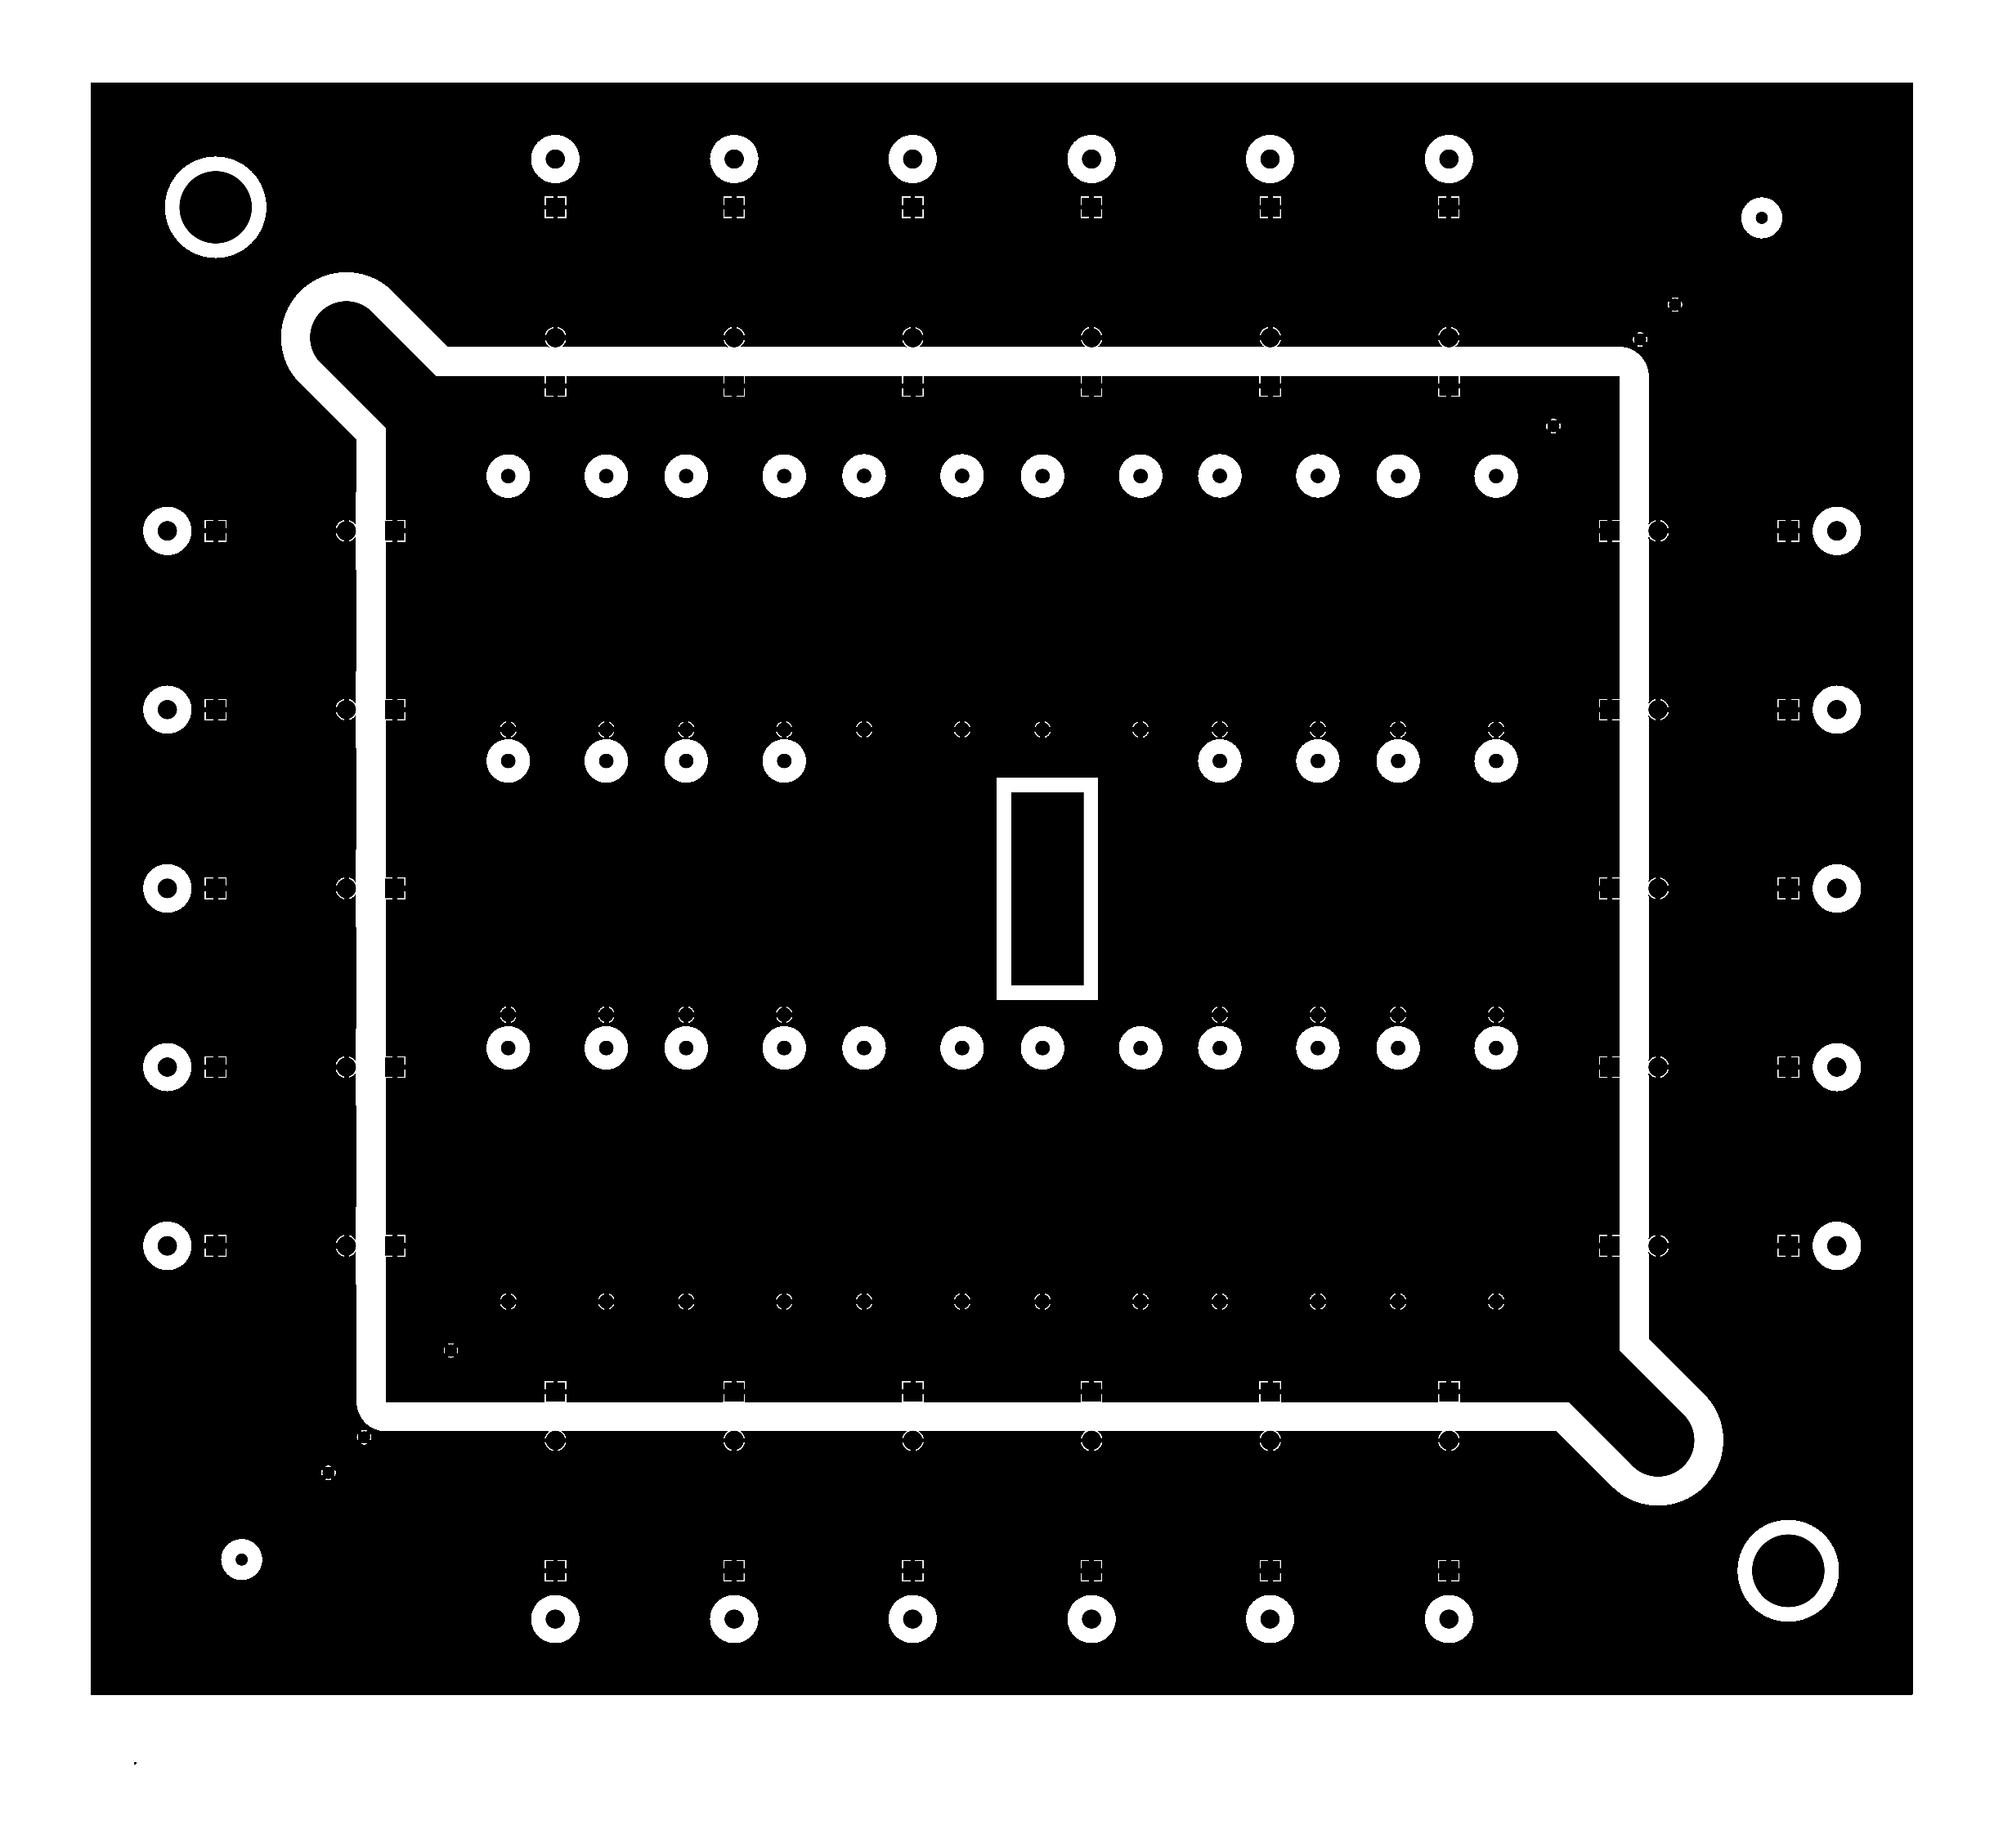
\includegraphics[width=\textwidth]{pcb_medziobvod_top}
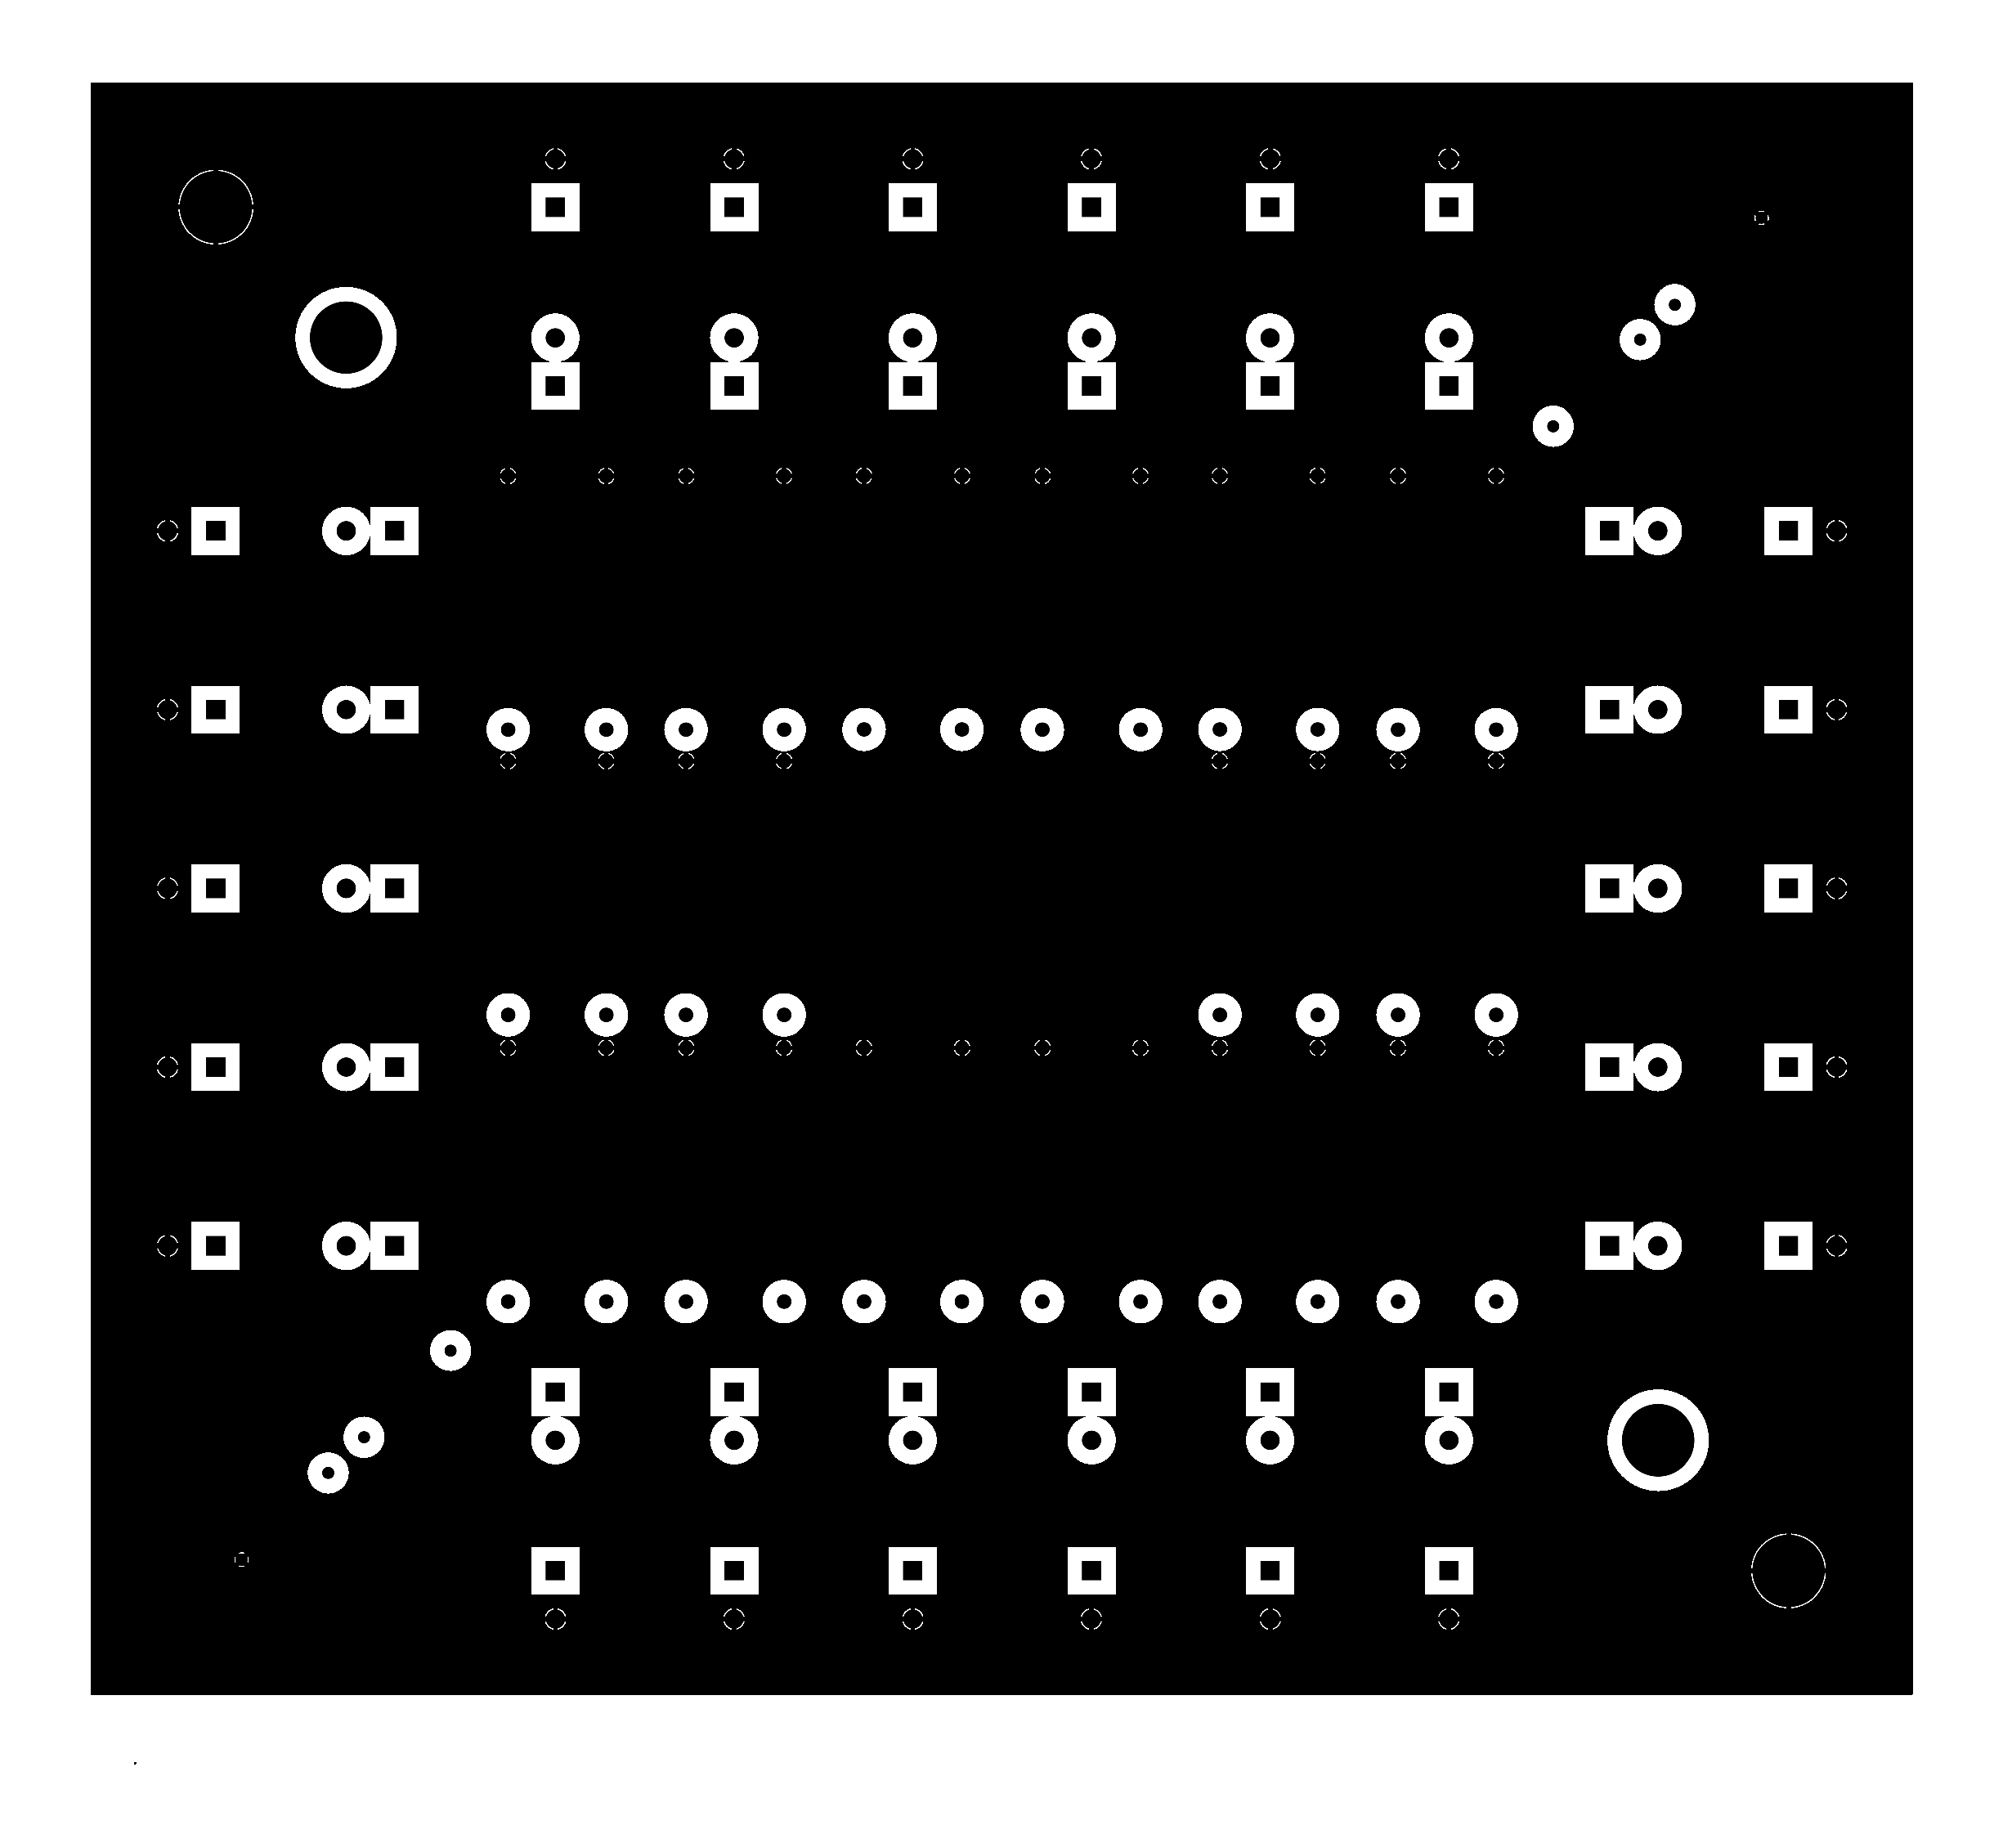
\includegraphics[width=\textwidth]{pcb_medziobvod_bot}
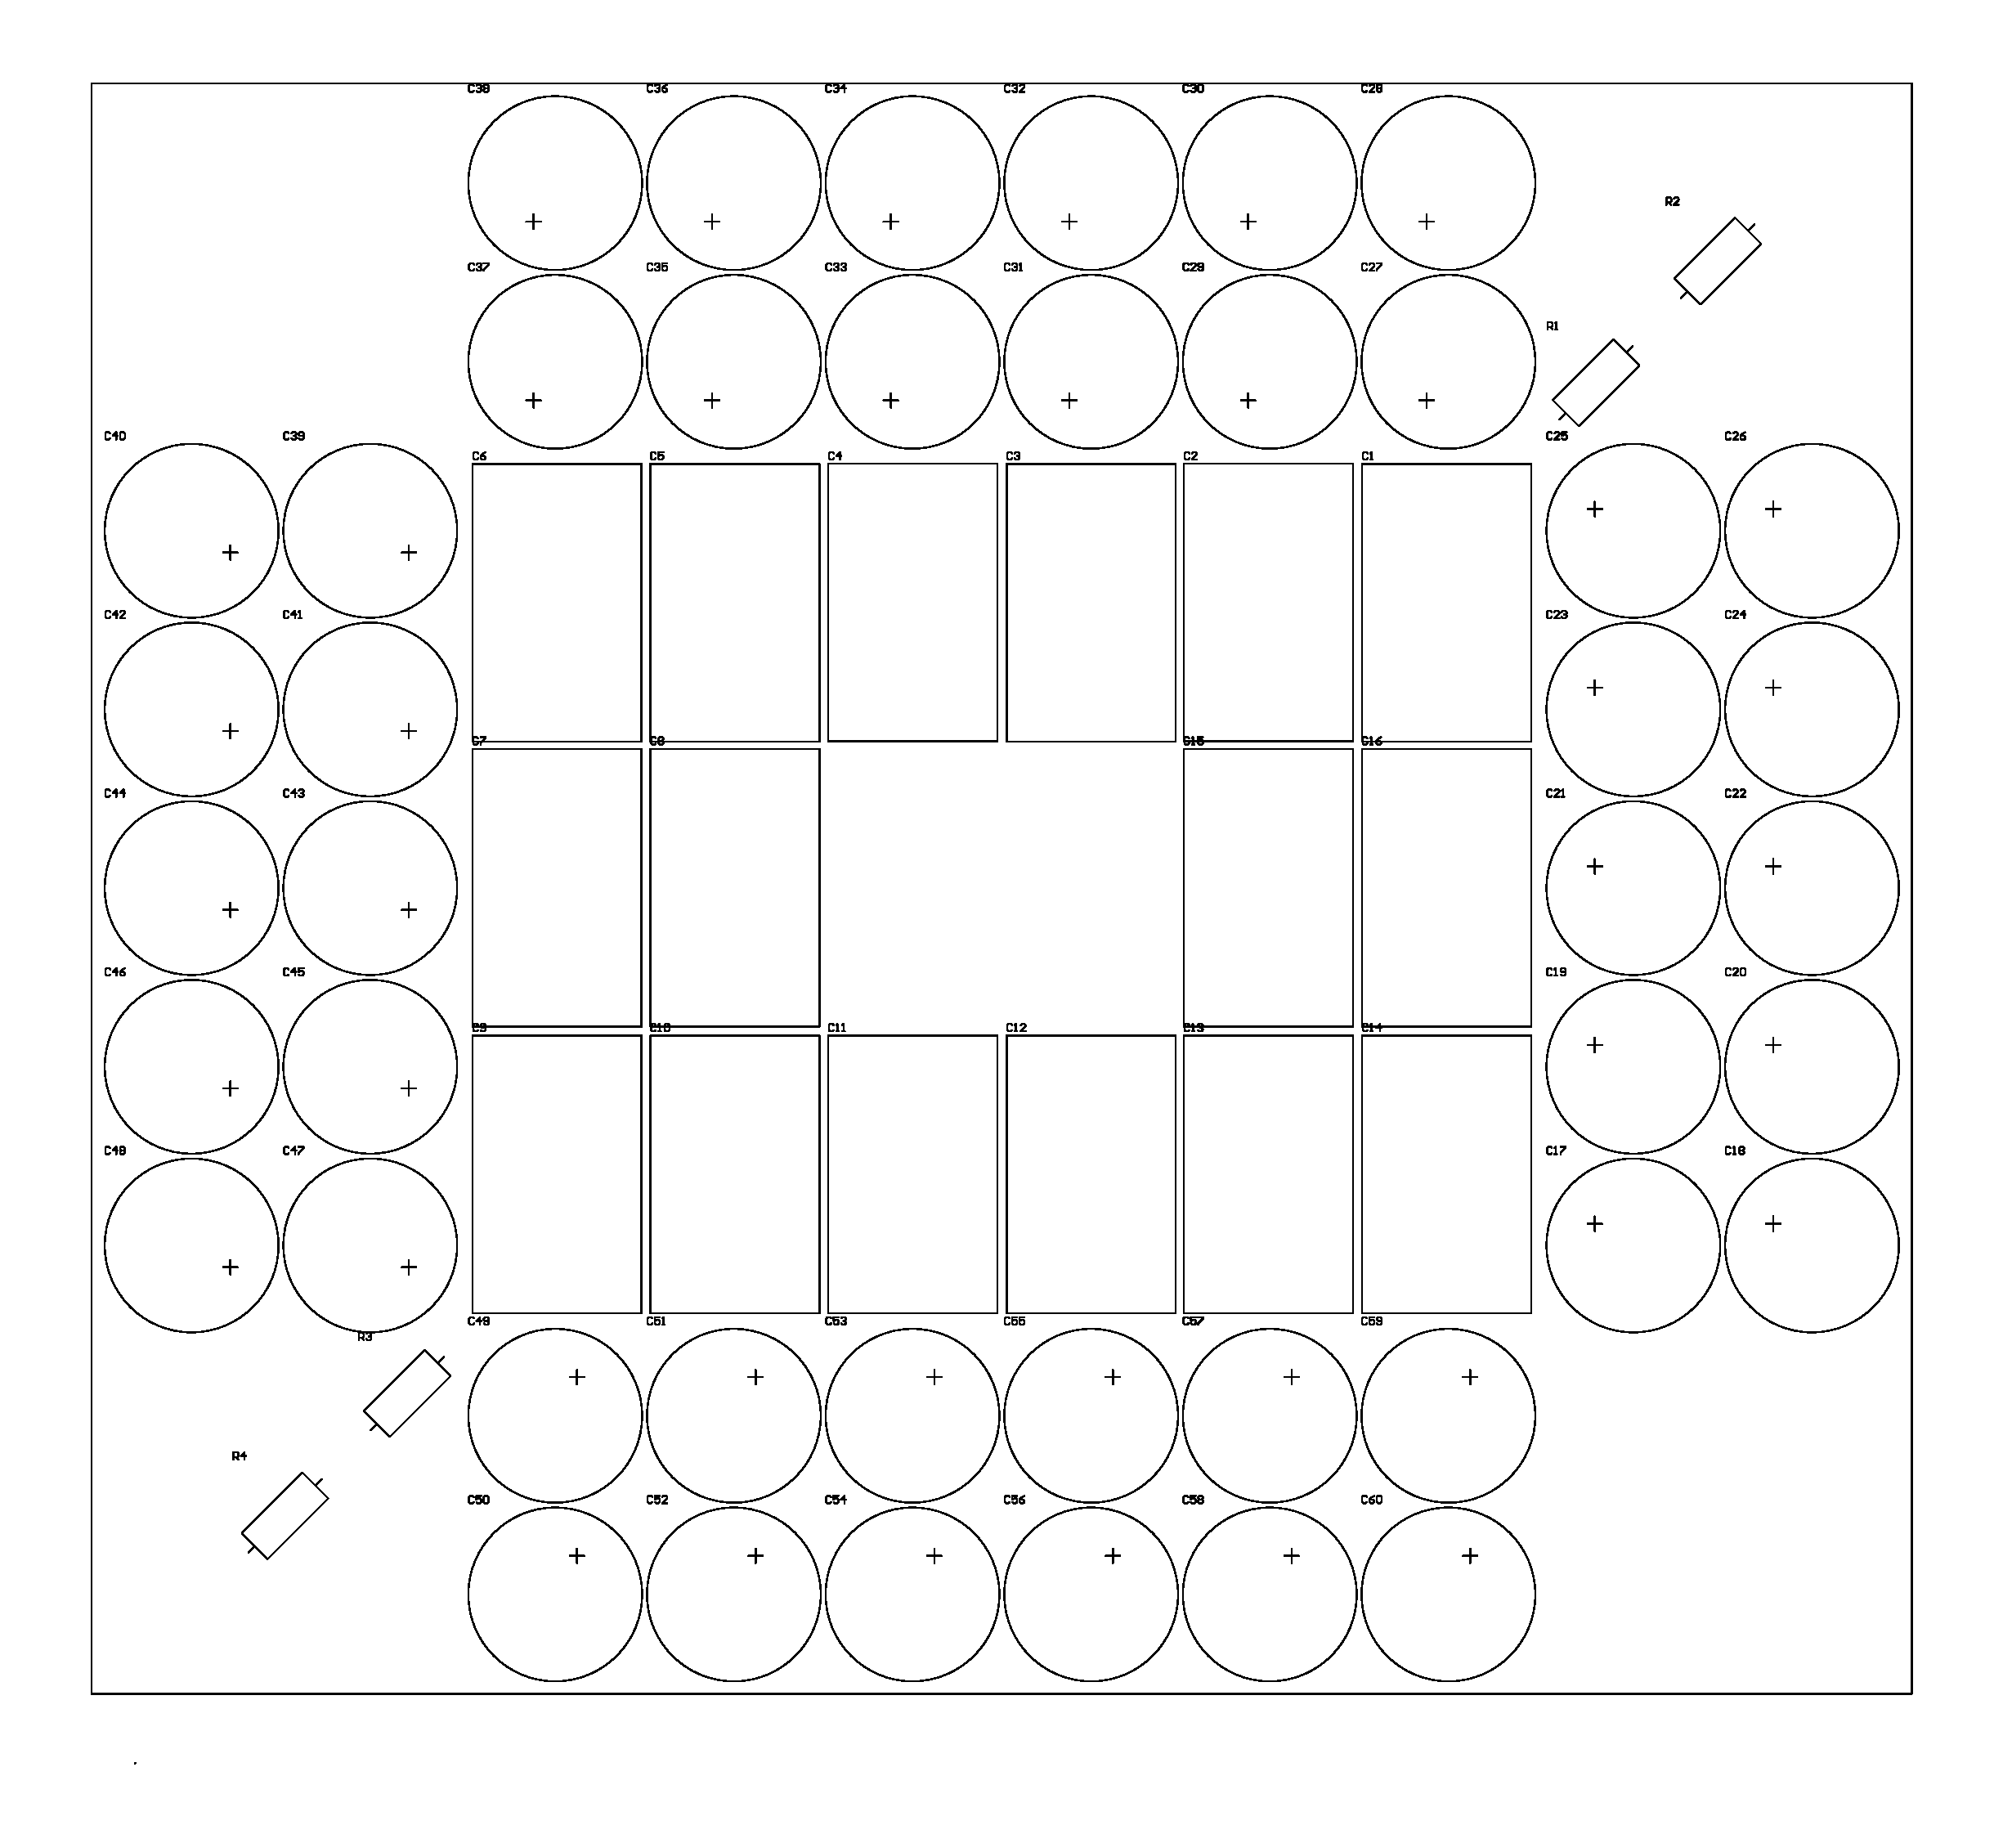
\includegraphics[width=\textwidth]{pcb_medziobvod_bot_ass}

%\newpage
%\subsection{Zoznam súčiastok}
%\small
%\hspace{2cm}
%\begin{verbatim}
%\end{verbatim}
\normalsize


\chapter{Zdrojové kódy pre simulácie} \label{ch:priloha_sim}

\section{\textsc{Spice} - príklad netlistu}
\myfig{schema_input}{Príklad všeobecnej simulačnej schémy pre generovanie SPICE netlistu (vytvorená v programe Xcircuit).}{\label{fig:append_schema_input}}

\subsection{input.spc}

\begin{lstlisting}
*SPICE circuit <input> from XCircuit v3.8 rev 78

.include gce.sp
.include control.sp
C5 int4 int10 000p
C2 int7 ne 000p
L3 int10 nc 00n
Rd int11 int4 r='v(int11 ) > v(int4 ) ? .1u : 10MEG'
V1 int4 int5 303
L1 ne nepar 00n
Va1 nepar 0 0
R1 0 int5 0
Rce1 int7 ne r='1/v(ngce)'
L4 int11 int10 00n
L2 nc int7 000n
I1 int4 int10 10.3
C1 int7 0 000p
C3 int10 0 000p
C4 int10 int7 000p
C6 int4 int11 000p

.end
\end{lstlisting}

\newpage
\subsection{gce.sp}
(generované pomocou \textit{Octave})

\begin{lstlisting}
Btime ntime 0 v= 'time'

**************************************
*** vypocet gce podla mojej krivky ***
**************************************
Bgce ngce 0 v=
+	v(ntime) <0.0001948?
+		-3423555918453.736*0.0001948*0.0001948+ 1334502097.012*0.0001948+-130038.128
+	:v(ntime) <0.000195?
+		-3423555918453.736*v(ntime)*v(ntime)+ 1334502097.012*v(ntime)+-130038.128
+	:v(ntime) <0.00019515?
+		-270156826283465.4*v(ntime)*v(ntime)+105360477539.367*v(ntime)+-10272570.734
+	:v(ntime) <0.00019521?
+		602514803859639.9*v(ntime)*v(ntime)+-235243259705.487*v(ntime)+22961838.928
+	:v(ntime) <0.00019524?
+		156172912727445.8*v(ntime)*v(ntime)+-60982458569.656*v(ntime)+5953113.433
+	:v(ntime) <0.0001954?
+		155024509820.893*v(ntime)*v(ntime)+-60593578.438*v(ntime)+5920.972
+	:v(ntime) <0.0001957?
+		16666666667.291*v(ntime)*v(ntime)+-6523333.334*v(ntime)+638.309
+	:
+		16666666667.291*0.0001957*0.0001957+-6523333.334*0.0001957+638.309
**************************************
\end{lstlisting}


\subsection{control.sp}

(generované pomocou \textit{Octave})

\begin{lstlisting}
.control
tran 1.9e-09 0.0001962 0.0001943
set nobreak
print ngce nc i(Va1) > /tmp/patocka__/data.data
.endc
\end{lstlisting}


\newpage

\section{Knižnica \textit{Octave} (\textsc{Matlab}) funkcií pre generovanie modelu $g_{CE}$}

Vstupnými (zmeranými) datami je tabuľka vo forme (\ref{eq:tab_predpis_t012}), syntaxou Matlabu zapísaná do štruktúry:
\begin{verbatim}
tab_on.tus = [t0, t1, t2, t3];
tab_on.G = [G0, I1/U1, I2/U2, I3/U3];
tab_on.t = tab_on.tus * 1e-6;
\end{verbatim}
Z tabuľky sú funkciou \texttt{tab2abc} dopočítané konštanty vystupujúce vo vzťahu (\ref{eq:krivka_subintervaly_gong1g2goff}) a následne sú pomocou funkcie \texttt{write\_spice\_model} zapísané časovo závislé SPICE výrazy na jednotlivých intervaloch daných tabuľkou zapísané do súbora na disku, ktorý je neskôr zahrnutý do simulačného netlistu. Z prostredia \textit{Octave} alebo \textsc{Matlab} je tiež možné pomocou príkazu \texttt{system(command)} spustiť simulátor (príkazom pre operačný systém) a následne čítať a ďalej spracúvať výsledky simulácie.

\subsection*{compute\_and\_write\_spice\_model\_my.m}
\begin{lstlisting}
function ret = compute_and_write_spice_model_my(tab_t, tab_G, str_outfilename)
	ret.abc = abc = tab2abc(tab_t, tab_G);
	ret.writestatus = write_spice_model_my(tab_t, abc, str_outfilename);
endfunction
\end{lstlisting}

\subsection*{write\_spice\_model\_my.m}
\begin{lstlisting}
function ret = write_spice_model_my(tab_t, abc, str_filename)

	if((FID = fopen(str_filename, "w")) == -1)
		puts("nepodarilo sa otvorit subor: ");
		puts(str_filename);
		puts("\n");
		ret = -1;
	else
		ret =1;
	endif
	
	for i=1:numel(tab_t)
		eval(strcat("str_t", num2str(i-1), " = num2str(tab_t(", num2str(i), "));"));
	endfor
	
	for i=1:numel(abc)/3
		eval(strcat("str_a", num2str(i), " = num2str(abc(", num2str((i-1)*3+1), "));"));
		eval(strcat("str_b", num2str(i), " = num2str(abc(", num2str((i-1)*3+2), "));"));
		eval(strcat("str_c", num2str(i), " = num2str(abc(", num2str((i-1)*3+3), "));"));
	endfor

	
	fputs(FID, "Btime ntime 0 v= 'time'\n\n"); 
	
	fputs(FID, "**************************************\n*** vypocet gce podla mojej krivky ***\n**************************************\n");
	fputs(FID, "Bgce ngce 0 v=\n");
	fputs(FID, strcat("+\tv(ntime) < ", str_t0, "?\n"));
	fputs(FID, strcat("+\t\t", str_a1, "*", str_t0, "*", str_t0, "+", str_b1, "*", str_t0, "+", str_c1, "\n"));
	
	for i=1:numel(abc)/3
		str_ti = num2str(tab_t(i+1));
		str_ai = num2str(abc((i-1)*3+1));
		str_bi = num2str(abc((i-1)*3+2));
		str_ci = num2str(abc((i-1)*3+3));

		feval("fputs", FID, strcat("+\t:v(ntime) < ", str_ti, "?\n"));
		feval("fputs", FID, strcat("+\t\t", str_ai, "*v(ntime)*v(ntime)+", str_bi, "*v(ntime)+", str_ci, "\n"));
	endfor


	fputs(FID, "+\t:\n");


	feval("fputs", FID, strcat("+\t\t", str_ai, "*", str_ti, "*", str_ti, "+", str_bi, "*", str_ti, "+", str_ci, "\n"));
%	fputs(FID, strcat("+\t\t", str_a2, "*", str_t2, "*", str_t2, "+", str_b2, "*", str_t2, "+", str_c2, "\n"));
	fputs(FID, "**************************************\n");
	
	if(fclose(FID) == -1)
		puts("nepodarilo sa zatvorit subor: ");
		puts(str_filename);
		puts("\n");
		ret = -2;
	else
		ret = 2;
	endif
endfunction
\end{lstlisting}

\subsection*{tab2abc\_off.m}
\begin{lstlisting}
function abc = tab2abc_off(tab_t, tab_G)
	switch numel(tab_t)
		case(3)
			abc = tab2abc_off_2(tab_t, tab_G);
		case(4)
			abc = tab2abc_off_3(tab_t, tab_G);
		case(5)
			abc = tab2abc_off_4(tab_t, tab_G);
		case(6)
			abc = tab2abc_off_5(tab_t, tab_G);
		case(7)
			abc = tab2abc_off_6(tab_t, tab_G);
		otherwise
			error("malo alebo vela bodov v tabulke. mozne je od 3 do 7");
	endswitch
endfunction
\end{lstlisting}

\subsection*{tab2abc\_off\_2.m}
\begin{lstlisting}
function abc12= tab2abc_off_2(tab_t012, tab_G012)

	t0=tab_t012(1);
	t1=tab_t012(2);
	t2=tab_t012(3);
	G0=tab_G012(1);
	G1=tab_G012(2);
	G2=tab_G012(3);

	V = [G0; G1; G1; G2; 0; 0];

	M = [	t0^2,	t0,	1,	0,	0,	0;
		t1^2,	t1,	1,	0,	0,	0;
		0,	0,	0,	t1^2,	t1,	1;
		0,	0,	0,	t2^2,	t2,	1;
		2*t1,	1,	0,	-2*t1,	-1,	0;
		0,	0,	0,	2*t2,	1,	0];
	abc12 = X = M \ V;
endfunction
\end{lstlisting}

\subsection*{tab2abc\_on.m}
\begin{lstlisting}
function abc = tab2abc_on(tab_t, tab_G)
	switch numel(tab_t)
		case(3)
			abc = tab2abc_on_2(tab_t, tab_G);
		case(4)
			abc = tab2abc_on_3(tab_t, tab_G);
		case(5)
			abc = tab2abc_on_4(tab_t, tab_G);
		case(6)
			abc = tab2abc_on_5(tab_t, tab_G);
		case(7)
			abc = tab2abc_on_6(tab_t, tab_G);
		otherwise
			error("malo alebo vela bodov v tabulke. mozne je od 3 do 7");
	endswitch
endfunction
\end{lstlisting}

\subsection*{tab2abc\_on\_2.m}
\begin{lstlisting}
function abc12= tab2abc_on_2(tab_t012, tab_G012)

	t0=tab_t012(1);
	t1=tab_t012(2);
	t2=tab_t012(3);
	G0=tab_G012(1);
	G1=tab_G012(2);
	G2=tab_G012(3);

	V = [G0; G1; G1; G2; 0; 0];

	M = [	t0^2,	t0,	1,	0,	0,	0;
		t1^2,	t1,	1,	0,	0,	0;
		0,	0,	0,	t1^2,	t1,	1;
		0,	0,	0,	t2^2,	t2,	1;
		2*t1,	1,	0,	-2*t1,	-1,	0;
		2*t0,	1,	0,	0,	0,	0];
	abc12 = X = M \ V;
endfunction
\end{lstlisting}




%\chapter{Charakteristická impedancia a odrazy na dlhom vedení}

\lettrine{K}{oaxiálny} kábel prenášajúci signál v kmitočtovom pásme stoviek $\un{MHz}$ predstavuje dlhé vedenie ($l \geq \frac{\lambda}{4}$), \cite{tirpak} teda také, ktoré nemožno modelovať sústredením jeho parazitných parametrov do diskrétnych prvkov. Napätie i prúd sú preto funkciami času aj polohy; merné (na jednotku dĺžky) primárne parametre v prípade homogénneho vedenia nie sú funkciami polohy. Pozdĺžne parametre $R \un{[\Ohm/m]}$, $L\un{[H/m]}$ dopredného a spätného vodiča možno bez dopustenia sa principiálnej chyby sústrediť do jedného vodiča. Vznikne tak obvod pozostávajúci z elementov dĺžky $\dif x$, ako na Obr. \ref{fig:vedenie}.

\begin{figure}[!ht]
	\centering
	% XCircuit output "vedenie.tex" for LaTeX input from vedenie.ps
\def\putbox#1#2#3#4{\makebox[0in][l]{\makebox[#1][l]{}\raisebox{\baselineskip}[0in][0in]{\raisebox{#2}[0in][0in]{\scalebox{#3}{#4}}}}}
\def\rightbox#1{\makebox[0in][r]{#1}}
\def\centbox#1{\makebox[0in]{#1}}
\def\topbox#1{\raisebox{-0.60\baselineskip}[0in][0in]{#1}}
\def\midbox#1{\raisebox{-0.20\baselineskip}[0in][0in]{#1}}
   \scalebox{0.8}{
   \normalsize
   \parbox{5.88583in}{
   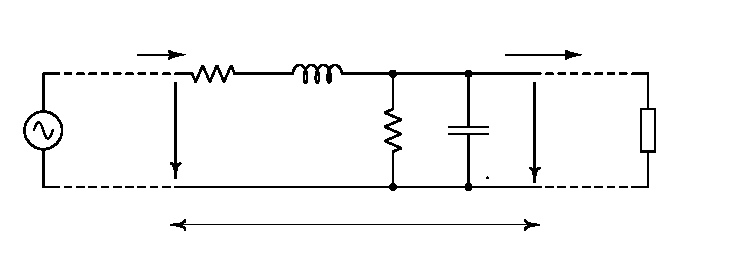
\includegraphics[scale=1.25]{vedenie}\\
   % translate x=237 y=229 scale 0.28
   \putbox{2.43in}{1.52in}{1.20}{\llaL}%
   \putbox{4.00in}{1.64in}{1.20}{\llaidi}%
   \putbox{1.52in}{1.52in}{1.20}{\llaR}%
   \putbox{3.25in}{0.97in}{1.20}{\llaG}%
   \putbox{3.88in}{0.97in}{1.20}{\llaC}%
   \putbox{0.42in}{0.81in}{1.20}{\llaGen}%
   \putbox{5.38in}{0.81in}{1.20}{\llaZat}%
   \putbox{4.36in}{0.81in}{1.20}{\llaudu}%
   \putbox{1.36in}{0.81in}{1.20}{\llau}%
   \putbox{1.09in}{1.64in}{1.20}{\llai}%
   \putbox{2.58in}{0.14in}{1.20}{\lladx}%
   } % close 'parbox'
   } % close 'scalebox'
   \vspace{-\baselineskip} % this is not necessary, but looks better

	\caption{Element dĺžky $\dif x$ vedenia s rozloženými parametrami.}
	\label{fig:vedenie}
\end{figure}
Z Kirchhoffových rovníc a následného separovania premenných (rovnica zvlášť pre $(i(x,t)$ resp. $u(x,t)$) vyplývajú známe telegrafné rovnice.
Pre výrazné matematické zjednodušenie (prechod od parciálnych k obyčajným diferenciálnym rovniciam) je možné hoci aj na úkor všeobecnosti zaviesť technicky zmysluplný predpoklad harmonických priebehov veličín a namiesto časových derivácii a integrácii využiť symbolickú metódu koplexného operátora $j \omega$. Potom:

\begin{subequations} \label{eq:vedenie_harm_kirch}
	\begin{align}
	\dxdtp{\cpx{U}}{x} \dif x = R \cdot \cpx{I} \cdot \dif x + j\omega L \cdot \cpx{I} \cdot \dif x\\
	\dxdtp{\cpx{I}}{x} \dif x = G \cdot \cpx{U} \cdot \dif x + j\omega C \cdot \cpx{U} \cdot \dif x
\end{align}
\end{subequations}

Vynásobením rovníc (\ref{eq:vedenie_harm_kirch}) faktorom $\frac{1}{\dif x}$ dostávame:

\begin{subequations} \label{eq:vedenie_harm_duidx}
	\begin{align}
		\dxdtp{\cpx{U}}{x} = (R + j\omega L) \cdot \cpx{I} = \cpx{Z} \cdot \cpx{I} \label{eq:vedenie_harm_duidx_U'=Z.I}\\
		\dxdtp{\cpx{I}}{x} = (G + j\omega C) \cdot \cpx{I} = \cpx{Y} \cdot \cpx{U} \label{eq:vedenie_harm_duidx_I'=Y.U}
\end{align}
\end{subequations}

Vyjadrením $\dxdtp{\cpx{U}}{x} = \dxdtp{^2\cpx{I}}{x^2} \cdot \frac{1}{\cpx{Y}}$ z (\ref{eq:vedenie_harm_duidx_I'=Y.U}) a dosadením do (\ref{eq:vedenie_harm_duidx_U'=Z.I}) a naopak dostávame \textbf{telegrafné rovnice pre harmonické priebehy}:

\begin{subequations} \label{eq:telegraf_harm}
	\begin{align}
		\dxdtp{^2\cpx{I}}{x^2} = \cpx{Z}\cpx{Y} \cdot \cpx{I} \label{eq:telegraf_harm_i}\\
		\dxdtp{^2\cpx{U}}{x^2} = \cpx{Z}\cpx{Y} \cdot \cpx{U} \label{eq:telegraf_harm_u}
	\end{align}
\end{subequations}
Riešením rovnice $\dxdtp{^2\cpx{U}}{x^2} - \cpx{Z}\cpx{Y} \cdot \cpx{U} = 0$, tj. (\ref{eq:telegraf_harm_u}) je:

\begin{equation}
	\cpx{U}(x) = \cpx{U}_{0+} \cdot e^{\sqrt{\cpx{Z}\cpx{Y}} \cdot x} + \cpx{U}_{0-} \cdot e^{-\sqrt{\cpx{Z}\cpx{Y}} \cdot x}
	\label{eq:telegraf_riesenie_u}
\end{equation}

Komplexné časovo natáčajúce sa fázory $\cpx{U}_{0+}$ a  $\cpx{U}_{0+}$ predstavujú harmonické vlnenie, exponenciálne členy predstavujú útlm amplitúdy pozdĺž vedenia, a to v doprednom resp. spätnom smere. Hovoríme o priamej a odrazenej vlne. Výsledná vlna je superpozíciou priamej a odrazenej vlny.

Dosadením riešenia (\ref{eq:telegraf_riesenie_u}) do (\ref{eq:vedenie_harm_duidx_U'=Z.I}) získavame výraz pre prúdovú vlnu:

\begin{equation}
	\cpx{I}(x) = \frac{1}{\cpx{Z}} \dxdtp{\cpx{U}}{x} = \frac{1}{\cpx{Z}} \sqrt{\cpx{Z}\cpx{Y}} \left( \cpx{U}_{0+} \cdot e^{\sqrt{\cpx{Z}\cpx{Y}} \cdot x} - \cpx{U}_{0-} \cdot e^{-\sqrt{\cpx{Z}\cpx{Y}} \cdot x} \right)
	\label{eq:telegraf_harm_riesenie_i}
\end{equation}

Výrazu
\begin{equation}
	\sqrt{\frac{\cpx{Z}}{\cpx{Y}}} = \cpx{Z}_0
	\label{eq:char_impedancia}
\end{equation}
sa hovorí \textbf{charakteristická (vlnová) impedancia vedenia}.

Potom výrazy pre napäťovú (\ref{eq:telegraf_riesenie_u}) a prúdovu (\ref{eq:telegraf_harm_riesenie_i}) vlnu nadobudnú tvar:

\begin{subequations} 
	\label{eq:telegraf_harm_riesenia_obe}
	\begin{align}
		\cpx{U}(x) = \cpx{U}_{0+} \cdot e^{\sqrt{\cpx{Z}\cpx{Y}} \cdot x} + \cpx{U}_{0-} \cdot e^{-\sqrt{\cpx{Z}\cpx{Y}} \cdot x}
	\label{eq:telegraf_harm_riesenia_obe_u}\\
		\cpx{I}(x) = \frac{1}{\cpx{Z}_0} \left( \cpx{U}_{0+} \cdot e^{\sqrt{\cpx{Z}\cpx{Y}} \cdot x} - \cpx{U}_{0-} \cdot e^{-\sqrt{\cpx{Z}\cpx{Y}} \cdot x} \right)
	\label{eq:telegraf_harm_riesenia_obe_i}
	\end{align}
\end{subequations}

Výrazy $\cpx{U}_{0+}$, $\cpx{U}_{0-}$ predstavujú okrajové podmienky riešenia To všeobecne neznamená že by priamo vyjadrovali konkrétnu fyzikálnu alebo merateľnú kvantitu ako napr. vstupné alebo výstupné napätie na vedení. Dosadením známeho vstupného ($x=0$) alebo výstupného ($x=l$) napätia a prúdu do (\ref{eq:telegraf_harm_riesenia_obe}) sa však dajú jednoznačne vyjadriť.

Zámerom je \uv{nastavenie} okrajových podmienok tak, aby nedochádzalo na vedení k odrazom.
Výstupné napätie považujme za dané; výstupný prúd bude potom určený výstupnou impedanciou: $i_{výst} = \frac{u_{výst}}{Z_{výst}}$, resp.:
\begin{equation}
	\cpx{I}_{výst} = \frac{\cpx{U}_{výst}}{\cpx{Z}_{výst}}
	\label{eq:Ivyst=Uvyst/Zvyst}
\end{equation}

Dosadením daného výstupného napätia $\cpx{U}(l) = \cpx{U}_{výst}$ do (\ref{eq:telegraf_harm_riesenia_obe_u}) dostávame:
\begin{equation}
	\cpx{U}_{výst} = \cpx{U}_{0+} \cdot e^{\sqrt{\cpx{Z}\cpx{Y}} \cdot l} + \cpx{U}_{0-} \cdot e^{-\sqrt{\cpx{Z}\cpx{Y}} \cdot l}
	\label{eq:telegraf_Uvyst}
\end{equation}

Ďalej dosadením (\ref{eq:telegraf_Uvyst}) do (\ref{eq:Ivyst=Uvyst/Zvyst}) vyjadríme:
\begin{equation}
	\cpx{I}_{výst} = \frac{1}{\cpx{Z}_{výst}} \left( \cpx{U}_{0+} \cdot e^{\sqrt{\cpx{Z}\cpx{Y}} \cdot l} + \cpx{U}_{0-} \cdot e^{-\sqrt{\cpx{Z}\cpx{Y}} \cdot l} \right)
	\label{eq:telegraf_Ivyst=Uvyst/Z_vyst}
\end{equation}

a zároveň platí telegrafná rovnica (\ref{eq:telegraf_harm_riesenia_obe_i}):
\begin{equation}
	\cpx{I}_{výst} = \frac{1}{\cpx{Z}_0} \left( \cpx{U}_{0+} \cdot e^{\sqrt{\cpx{Z}\cpx{Y}} \cdot l} - \cpx{U}_{0-} \cdot e^{-\sqrt{\cpx{Z}\cpx{Y}} \cdot l} \right)
	\label{eq:telegraf_Ivyst}
\end{equation}

Porovnaním pravých strán (\ref{eq:telegraf_Ivyst=Uvyst/Z_vyst}) a (\ref{eq:telegraf_Ivyst}) dostávame vzťah:

\begin{equation}
	\frac{1}{\cpx{Z}_{výst}} \left( \cpx{U}_{0+} \cdot e^{\sqrt{\cpx{Z}\cpx{Y}} \cdot l} + \cpx{U}_{0-} \cdot e^{-\sqrt{\cpx{Z}\cpx{Y}} \cdot l} \right)
	=
	\frac{1}{\cpx{Z}_0} \left( \cpx{U}_{0+} \cdot e^{\sqrt{\cpx{Z}\cpx{Y}} \cdot l} - \cpx{U}_{0-} \cdot e^{-\sqrt{\cpx{Z}\cpx{Y}} \cdot l} \right)
	\label{eq:Ivyst_prave_strany}
\end{equation}

I bez toho, aby sme vyjadrovali výrazy $\cpx{U}_{0+}$, $\cpx{U}_{0-}$ sa dá z rovnice (\ref{eq:Ivyst_prave_strany}) usúdiť chovanie na vedení za určitých hraničných podmienok.

Pri výstupe vedenia naprázdno bude $Z_{výst} \to \infty$, čiže výraz na pravej strane  (\ref{eq:Ivyst_prave_strany}) bude nulový. Potom aj ľavá strana bude rovná nule a na vedení vzniká stojaté vlnenie \footnote{koeficient odrazu definovaný ako pomer odrazenej a priamej vlny (v každom bode pozdĺž osi x) je na konci vedenia naprázdno rovný jednotke.}. Tejto situácii približne zodpovedá pripojenie vedenia na $1\un{M\Ohm}$ vstupný odpor osciloskopu.

Pokiaľ požadujeme na konci vedenia neprítomnosť odrazov, pričom primárne parametre vedenia sú dané jeho konštrukciou (u koaxiálneho kábla $Z_0 = 50\Ohm$) a dĺžka $l$ je pevná, potom je nutné upraviť vstupnú impedanciu osciloskopu, a to takým spôsobom, aby mala rovnica sústavy riešenie práve vtedy, keď $\cpx{U}_{0-} = 0$.
 $\cpx{U}_{0-} = 0$ preto dosadíme do (\ref{eq:Ivyst_prave_strany}) a získavame známy vzťah pre prispôsobenie na výstupe vedenia:
\begin{equation}
	\cpx{Z}_{výst} = 
	\cpx{Z}_0 \frac{\cpx{U}_{0+}\cdot e^{\sqrt{\cpx{Z}\cpx{Y}}\cdot l}}{\cpx{U}_{0+}\cdot e^{\sqrt{\cpx{Z}\cpx{Y}}\cdot l}} =
	\cpx{Z}_0 = 50\un{\Ohm}
	\label{eq:Zvyst=Z0}
\end{equation}

Obdobným spôsobom je možné odvodiť ekvivalentný vzťah pre prispôsobenie na vstupe vedenia.


\label{LastPage}



%%%%%%%%
% pokusy
%%%%%%%%

%\myfig{aaaa}{pokusny-myfig}{aaaa}



\end{document}
